\documentclass[pdftex,11pt,a4paper,twoside]{report}

\usepackage{pdf_course_profile}

%\title{Cours d'�lectricit�}

\title{\begin{flushright}
    \rule{15cm}{1mm}\\
    \vspace{8mm}
    \huge{\bf{Electricit�}}\\
    \rule{15cm}{1mm}\\
    \large{Cours du CNAM - CPDA 1�re ann�e - 2006/2007}\\
    \today\\
    \small{Version 0.3.2}\\
    \end{flushright}
}

\author{Guillaume Pellerin / Christophe Langrenne\\
	CNAM - Chaire d'Acoustique\\
    5, rue du Vertbois F-75003 Paris\\
    \emph{guillaume.pellerin@cnam.fr}
}

\begin{document}

\maketitle
\newpage


Ce cours est destin� � introduire les notions g�n�rales d'�lectricit� pour la formation dispens�e par le \textbf{Centre de Pr�paration au Diplome d'Etat d'Audioproth�siste} (CPDA) au sein du Conservatoire National des Arts et M�tiers (CNAM) de Paris.

De nombreux �l�ments de ce polycopi� ont �t� tir�s des cours personnels de Christophe Langrenne, Ing�nieur de Recherche � la Chaire d'Acoustique du CNAM. Je le remercie vivement.\newline

Trois chapitres se distinguent. Tout d'abord les �l�ments th�oriques qui fondent la physique \textbf{�lectrostatique} sont abord�s. On y d�fini les charges, les champs et les potentiels �lectriques. Les interactions mutuelles entre les charges sont ici d�nu�es de tout mouvement m�canique. Un chapitre sur l'\textbf{�lectrocin�tique} introduit ensuite les effets �lectriques d�s aux mouvements �ventuels de ces charges qui produisent les courants continus �lectriques. Le troisi�me chapitre pr�sente ensuite les notions fondamentales de l'\textbf{�lectomagn�tisme} qui participent aux int�ractions entre les charges �lectriques sous l'effet des champs magn�tiques. Enfin, le dernier chapitre tente une synth�se de l'ensemble de ces effets pour d�finir les r�gles pratiques de calcul des circuits dans le cas des \textbf{courants variables}, notamment celui des courants alternatifs.\newline

On notera l'importance des s�ances de travaux dirig�s compl�mentaires pour cerner l'ensemble des m�thodes de calcul abord�es lors de ce  cours d'Electricit�.

Ce document est en constante �volution. Certaines parties seront donc revues ou corrig�es r�guli�rement. La version la plus r�cente peut �tre t�l�charg�e � tout moment � l'adresse web indiqu�e en page de garde.


\begin{figure}[b]
  
\includegraphics[clip=true,scale=0.7]{figures/logocnam_3.png}
  \large{Copyright (C) 2006-2007 Guillaume Pellerin}
\end{figure}

\newpage

\setcounter{page}{3}
\tableofcontents
\cleardoublepage
\renewcommand{\labelitemi}{$\bullet$}

%%%%%%%%%%%%%%%%%%%%%%%%%%%%

\chapter{Electrostatique}\label{chap_elecstat}
\section{G�n�ralit�s}

\subsection{La charge �lectrique �l�mentaire}

Une des manifestations quotidiennes de l'effet de l'�lectricit� statique est l'attraction mutuelle de petits corps l�gers avec des corps de plus grance masse. Une exp�rience bien connue consiste par exemple � attirer un bout de papier avec une baguette m�tallique pr�alablement frott�e par un morceau de laine. Ce type de ph�nom�ne est connu depuis longtemps et m�me rapport� par Thal�s de Milet vers 600 av. J.-C. Ce dernier observa en effet un d�placement spontan� de brindilles de paille vers un morceau de ambre jaune\footnote{L'ambre jaune est une sorte de r�sine fossilis�e.} pr�alablement frott�. Le mot \textbf{�lectricit�} provient d'ailleurs du mot grec \emph{�lektron} qui signifie ambre.

L'�tude des ph�nom�nes �lectriques a continu� jusqu'au XIX�me si�cle o� il a �t� �labor� la th�orie unifi�e des ph�nom�nes �lectriques et magn�tiques, appel�e \textbf{�lectromagn�tisme}.

%On se contentera pour l'instant de prendre l'habitude de parler de ph�nom�nes \underline{�lectrostatiques}.\\

\subsubsection{Observations d'apr�s l'exp�rience.}

Dans la nature, on explique l'ensemble des effets d'�lectricit� statique par l'existence de particules portant une charge $q$ positive ou n�gative. Les �l�ments dont les charges sont de m�mes signes se repoussent tandis que les �l�ments dont les charges sont de signes oppos�s s'attirent.

La mati�re est en effet constitu�e d'atomes, ces atomes �tant eux-m�mes constitu�s de particules �l�mentaires : les \textbf{�lectrons}, les \textbf{protons} et les \textbf{neutrons}. Les �lectrons gravitent autour du noyau constitu� de neutrons et de protons. Ces trois types de particules poss�dent des propri�t�s diff�rentes comme par exemple leur masses ou leur charges �lectriques respectives. Dans le syst�me d'unit� international, l'unit� de charge �lectrique est le \textbf{Coulomb} not� \textbf{C}.

\begin{center}
\begin{tabular}{lll}
Electron : & $q_{e} = -e = -1.602.10^{-19} \ \mathrm{C}$ & $m_{e}=9.109.10^{-31}\ \mathrm{kg}$ \\
Proton : & $q_{p} = e = 1.602.10^{-19} \ \mathrm{C}$ & $m_{p}=1.672.10^{-27}\ \mathrm{kg}$ \\
Neutron : & $q_{n} = 0 \ \mathrm{C}$ & $m_{p}=1.674.10^{-27}\ \mathrm{kg}$ \\
\end{tabular}
\end{center}

$e$ est la \textbf{charge �lectrique} �l�mentaire la plus petite qui puisse se manifester � l'�chelle atomique. Toutes les valeurs de charges possibles sont ainsi d�finies comme des multiples de $e$. Les quantit�s d'�lectrons et de protons contenues dans un mat�riau donn� d�terminent donc sa charge globale, fixe ou variable dans le temps, les �lectrons pouvant s'�chapper plus ou moins librement.
La charge �lectrique totale $q$ sera �gale � la somme alg�brique des charges �l�mentaires.

\subsubsection{Mat�riaux isolants et mat�riaux conducteurs.}

Un mat�riau est constitu� d'un grand nombre de charges �lectriques. Lorsque la charge totale n�gative est �gale � la charge totale positive, le mat�riau est dit �lectriquement neutre. Si des �lectrons s'�chappent ou sont arrach�s, la charge globale augmente et devient positive. Si des �lectrons sont ajout�s, la charge globale diminue et devient n�gative. Ces ph�nom�nes d�finissent l'effet d'\textbf{�lectrisation} des corps.

Un mat�riau est dit \textbf{conducteur parfait} si, lorsqu'il devient �lectris�, les �lectrons peuvent se d�placer librement dans tout le volume occup� par le mat�riau. Il sera un \textbf{isolant parfait} (ou \textbf{di�lectrique}) si les �lectrons sont incapables de se d�placer. Mais tous les mat�riaux ne sont pas totalement conducteurs ou isolants. Leurs propri�t�s de r�sistance � l'�lectrisation ou � la conduction, par les effets de frottement notamment, seront abord�es plus loin au chapitre \ref{chap_eleccine}.

\paragraph{Exp�rience~:}
Frotter vigoureusement une baguette m�tallique avec un chiffon, si possible en laine. Si elle est tenue � l'aide d'un mat�riau isolant, la baguette fini par attirer certains objets l�gers comme des plumes et de petits morceaux de papier. Le chiffon arrache en effet une certaine quantit� d'�lectrons � la surface de la baguette et l'�lectrise. En revanche, cette exp�rience n'a aucun effet si la baguette est tenue � pleine main. Le corps humain est en effet conducteur et donne les �lectrons manquants � la baguette pour r�tablir l'�quilibre �lectrostatique.

\subsubsection{Principe de Conservation.}

En �lectrostatique, la charge totale d'un corps isol� est consid�r�e constante dans le temps. Cette charge est �galement invariante par changement de rep�re, contrairement � la masse.


\subsection{Loi de Coulomb}

A l'aide d'une balance de torsion, Charles Auguste de Coulomb (1736-1806) a effectu� une s�rie de mesures qui lui a permis de d�terminer les propri�t�s de la force �lectrostatique exerc�e par une charge ponctuelle $q_{1}$ sur une autre charge ponctuelle $q_{2}$~:\\

\begin{enumerate}
\item{La force est radiale, c'est-�-dire, dirig�e selon la droite qui joind les deux charges.}
\item{La force est proportionnelle au produit des charges~: attractive si elles sont de signe oppos�, r�pulsive sinon.}
\item{La force varie comme l'inverse du carr� de la distance entre les deux charges.}
\end{enumerate}

\begin{figure}[h]
\begin{center}
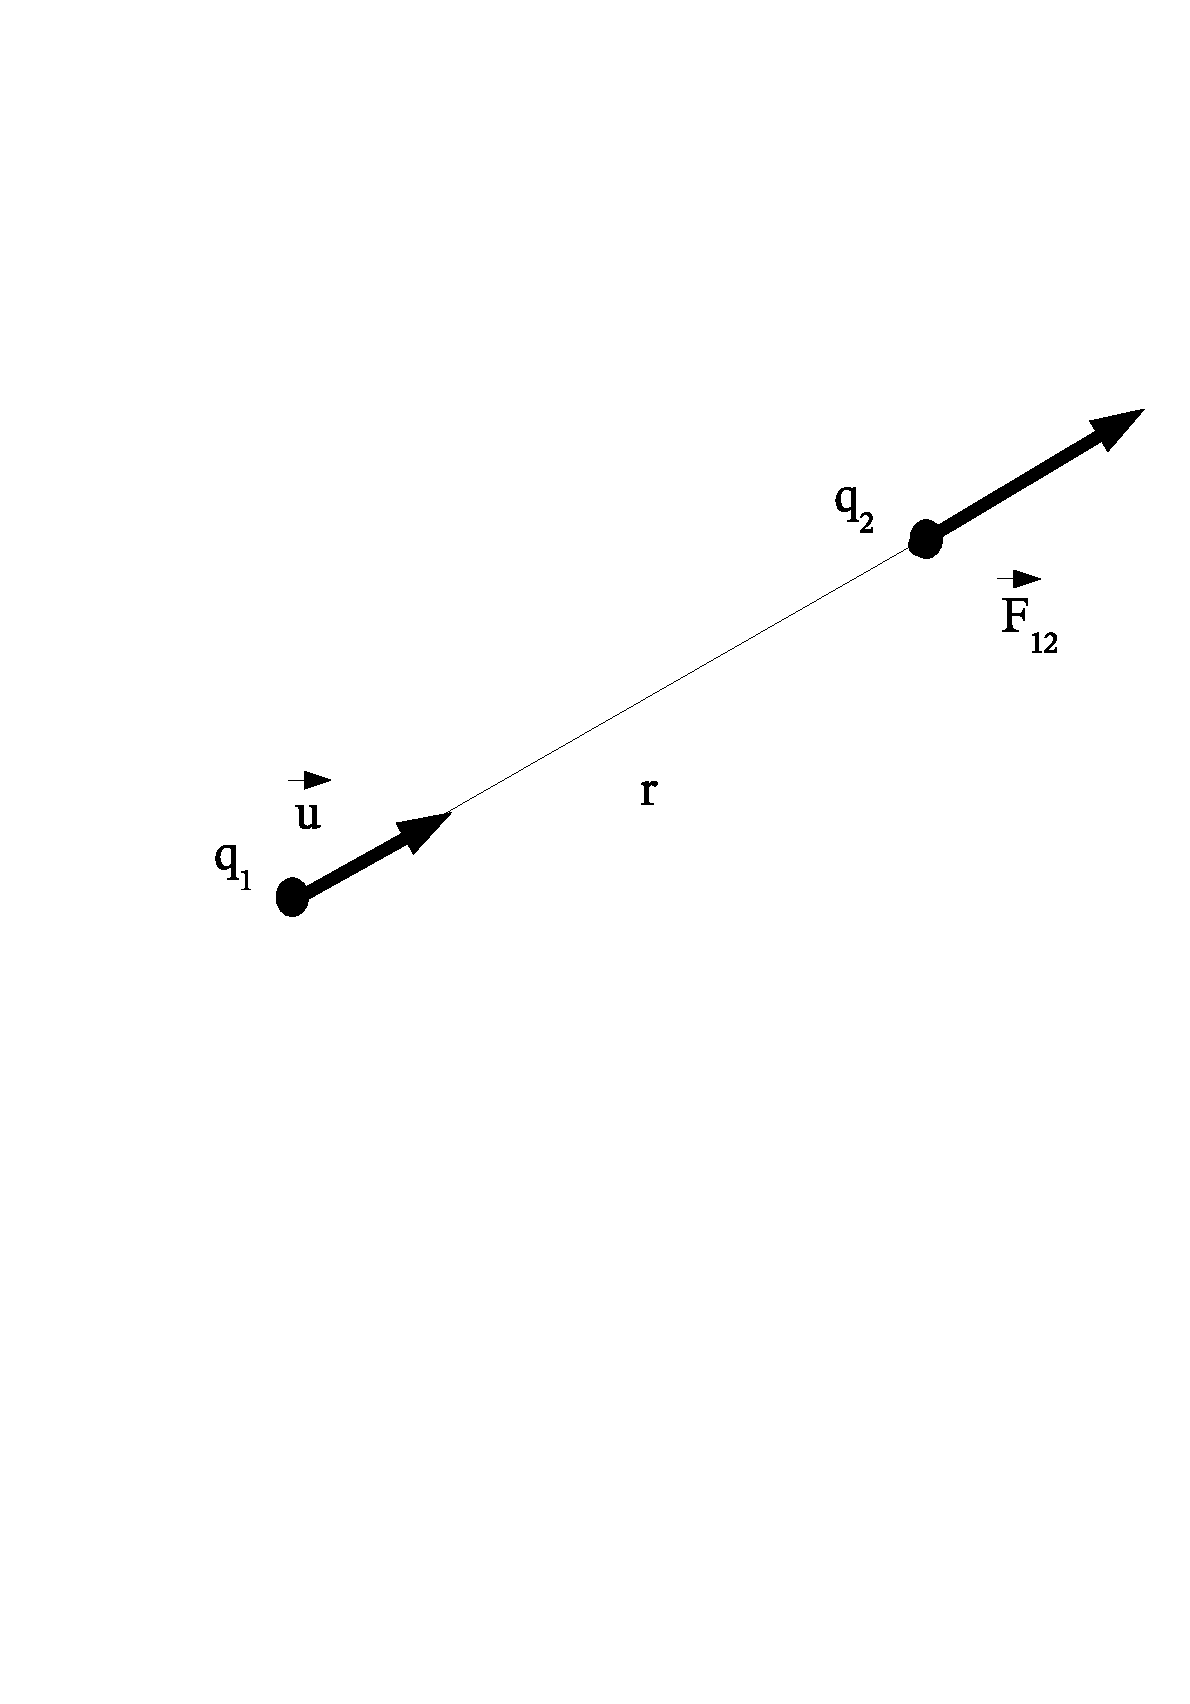
\includegraphics[clip=true,viewport=0cm 11cm 24cm 22cm,scale=0.3]{./figures/loi_de_coulomb.pdf}
\caption{Force de Coulomb exerc�e sur $q_{2}$ par $q_{1}$ (ici, les deux charges sont de m�mes signes).}
\end{center}
\end{figure}

L'expression math�matique moderne de la force de Coulomb traduisant ces propri�t�s est la suivante~:

\begin{equation}\label{coulomb}
\boxed{\vec{F}_{12}=\frac{1}{4\pi\varepsilon_{0}}\frac{q_{1}q_{2}}{r^{2}}\vec {u}}
\end{equation}

o� $\vec{u}$ est le vecteur unitaire parall�le � l'axe cr�� par les 2 charges et $\varepsilon_{0}=8,854187.10^{-12}\ \mathrm{F.m^{-1}}$ est la permittivit� du vide exprim�e en Farad/m�tre, \cad en $\mathrm{C^2.N^{-1}.m^{-2}}$. Ainsi, $\fractext{1}{4\pi\varepsilon_{0}}\approx 9.10^{9}\ \mathrm{N.m^{2}.C^{-2}}$.

\paragraph{Validit� de la loi de Coulomb.}
Cette expression n'est valable que dans le vide, pour des charges immobiles (approximation de l'�lectrostatique) et pour des distances sup�rieures � $10^{-14}\ \mathrm{m}$. Pour des distances plus faibles, les particules ne peuvent plus �tre consid�r�es ponctuelles.\\

La force �lectrostatique est � bien diff�rencier de la force gravitationnelle. Alors que la premiere d�pend de la charge �lectrique de chaque particule, la seconde d�pend uniquement de leur masse comme le montre la d�finition suivante.

\begin{defi}[Loi de gravitation universelle]
Soient $m_A$ et $m_B$ deux masses ponctuelles situ�es respectivement dans l'espace au points $A$ et $B$. La masse $m_A$ exerce spontan�ment une force d'attraction sur la masse $m_B$ telle que: .

\begin{equation}
\boxed{\vec{F}_{AB}=-G\frac{m_{A}m_{B}}{r^{2}}\vec{u}}
\end{equation}

o� $G=6.67 \ 10^{-11} \ N.m^{2}.kg^{-2}$ est la constante d'attraction universelle, $r=\Vert \overrightarrow{AB}\Vert$ et $\vec{u}=\overrightarrow{AB}/r$. Les valeurs de $m_A$ et $m_B$ �tant toujours positives, la force d'attraction est toujours attractive. On remarque que la masse $m_B$ exerce une force d'attraction oppos�e � $\vec{F}_{AB}$ : $\vec{F}_{BA}=-\vec{F}_{AB}$.
\end{defi}

\begin{rem}
Pour comparer l'influence des deux forces, calculons le rapport de la norme de la force �lectrostatique $\Vert \vec{F}_{E} \Vert$ et de la norme de la force gravitationnelle $\Vert \vec{F}_{G} \Vert$ intervenant entre deux protons ($m_{p}=1.6725 \ 10^{-27} \ kg$ et $q_p=1.6 \ 10^{-19} \ C$) :

$$\frac{F_E}{F_G}=1.24 \ 10^{36}.$$

Les forces �lectriques sont class�es dans les int�ractions fortes. Au niveau atomique, les forces de gravitation sont n�gligeables devant les forces �lectriques.
\end{rem}

\begin{bnote}[Pourquoi protons et �lectrons ne se collent-ils pas l'un contre l'autre ?]
%\bold{Pourquoi protons et �lectrons ne se collent-ils pas ensembles ?}\\
$\ $
\begin{itemize}
\item il existe d'autres forces � l'�chelle quantique : les forces nucl�aires sont plus fortes que les forces �lectriques, mais d�croissent plus rapidement (coh�sion des noyaux);
\item les �lectrons tournent autour du noyau compos� de neutrons et de protons et changent r�guli�rement d'orbite lorsqu'on leur apporte de l'�nergie;
\item l'effet quantique li� au principe d'incertitude.
\end{itemize}
\end{bnote}


\subsection{Champ �lectrostatique cr�� par une charge ponctuelle}

Soit une charge $q$ situ�e en un point $O$ de l'espace et $M$ un point quelconque de l'espace. La pr�sence de $q$ en $O$ modifie les propri�t�s �lectriques dans tout l'espace, notamment en $M$. On d�crit cet effet par l'existence d'un champ vectoriel $\vec{E}_1$ qui est le champ �lectrostatique issu de la loi de Coulomb et produit par la charge $q$.

\begin{defi}
Une particule de charge $q$ situ�e au point $O$ cr�� en tout point $M$ de l'espace distinct de $O$ un champ vectoriel $\vec{E}(M)$ appel� champ �lectrostatique et d'unit� le Volt/m�tre ($V.m^{-1}$) d�pendant de $r=\Vert\overrightarrow{OM}\Vert$ tel que :
\begin{equation}
\vec{E}(M)=\frac{1}{4\pi\varepsilon_{0}}\frac{q}{r^{2}}\vec{u}.
\end{equation}
\end{defi}

On peut ainsi r��crire l'�quation \ref{coulomb} sous la forme:

\begin{equation}
\vec{F}_{12}=q_{2}\vec{E}_1,
\end{equation}

avec

$$\vec{E}_1=\frac{1}{4\pi\varepsilon_{0}}\frac{q_1}{r^{2}}\vec{u}.$$

L'int�r�t de cette s�paration vient du fait que l'on distingue clairement ce qui d�pend uniquement de la particule qui subit la force (en $q_{2}$ dans l'exemple) de ce qui ne d�pend que d'une source ext�rieure (le vecteur $\vec{E}_{1}$ dans l'exemple).


\subsection{Principe de superposition}\label{princ_superpo}

Si il y a plus de deux charges en pr�sence, la force exerc�e sur une des charges est la somme vectorielle des forces de Coulomb exerc�es par chacune des autres charges. Ainsi, dans le cas d'un nuaga de charges ponctuelles,  le champ �lectrostatique au point quelconque $M$ s'�crit:

\begin{equation}
\boxed{\vec{E}(M)=\sum_{i=1}^n \frac{1}{4\pi\varepsilon_{0}}\frac{q_{i}}{r_{i}^{2}}\vec {u}_{i}.}
\end{equation}

\noindent o� $n$ est le nombre de particules.

En pratique, cette expression est rarement utilisable car les mat�riaux comportent un nombre gigantesque de particules. Consid�rant que les �chelles spatiales sont tr�s grandes devant les distances inter-particulaires, on perd alors toute possibilit� de distinguer une particule d'une autre. Il est donc souvent plus habile d'utiliser des distributions continues de charges.


\subsection{Distributions continues de charges}

Soit $P$ un point quelconque d'un espace conducteur $D$ et $\ud q$ la charge �l�mentaire concentr�e en ce point. Le champ �lectrostatique total cr�� en un point $M$ de l'espace par cette distribution de charge s'�crit~:

\begin{equation}
\boxed{\vec{E}(M)=\int_{D} \vec{\ud E}(M) \qquad \textrm{avec} \qquad \vec{\ud E}(M)=\frac{1}{4\pi\varepsilon_{0}}\frac{\ud q}{r^{2}}\vec {u}.}
\end{equation}

On a �galement pos� $r=\Vert \overrightarrow{PM} \Vert$ et $\overrightarrow{PM}=r\vec{u}$. Il s'agit �videmment d'une approximation, permettant de remplacer une somme presque infinie par une int�grale.


\begin{figure}[h]
\begin{center}
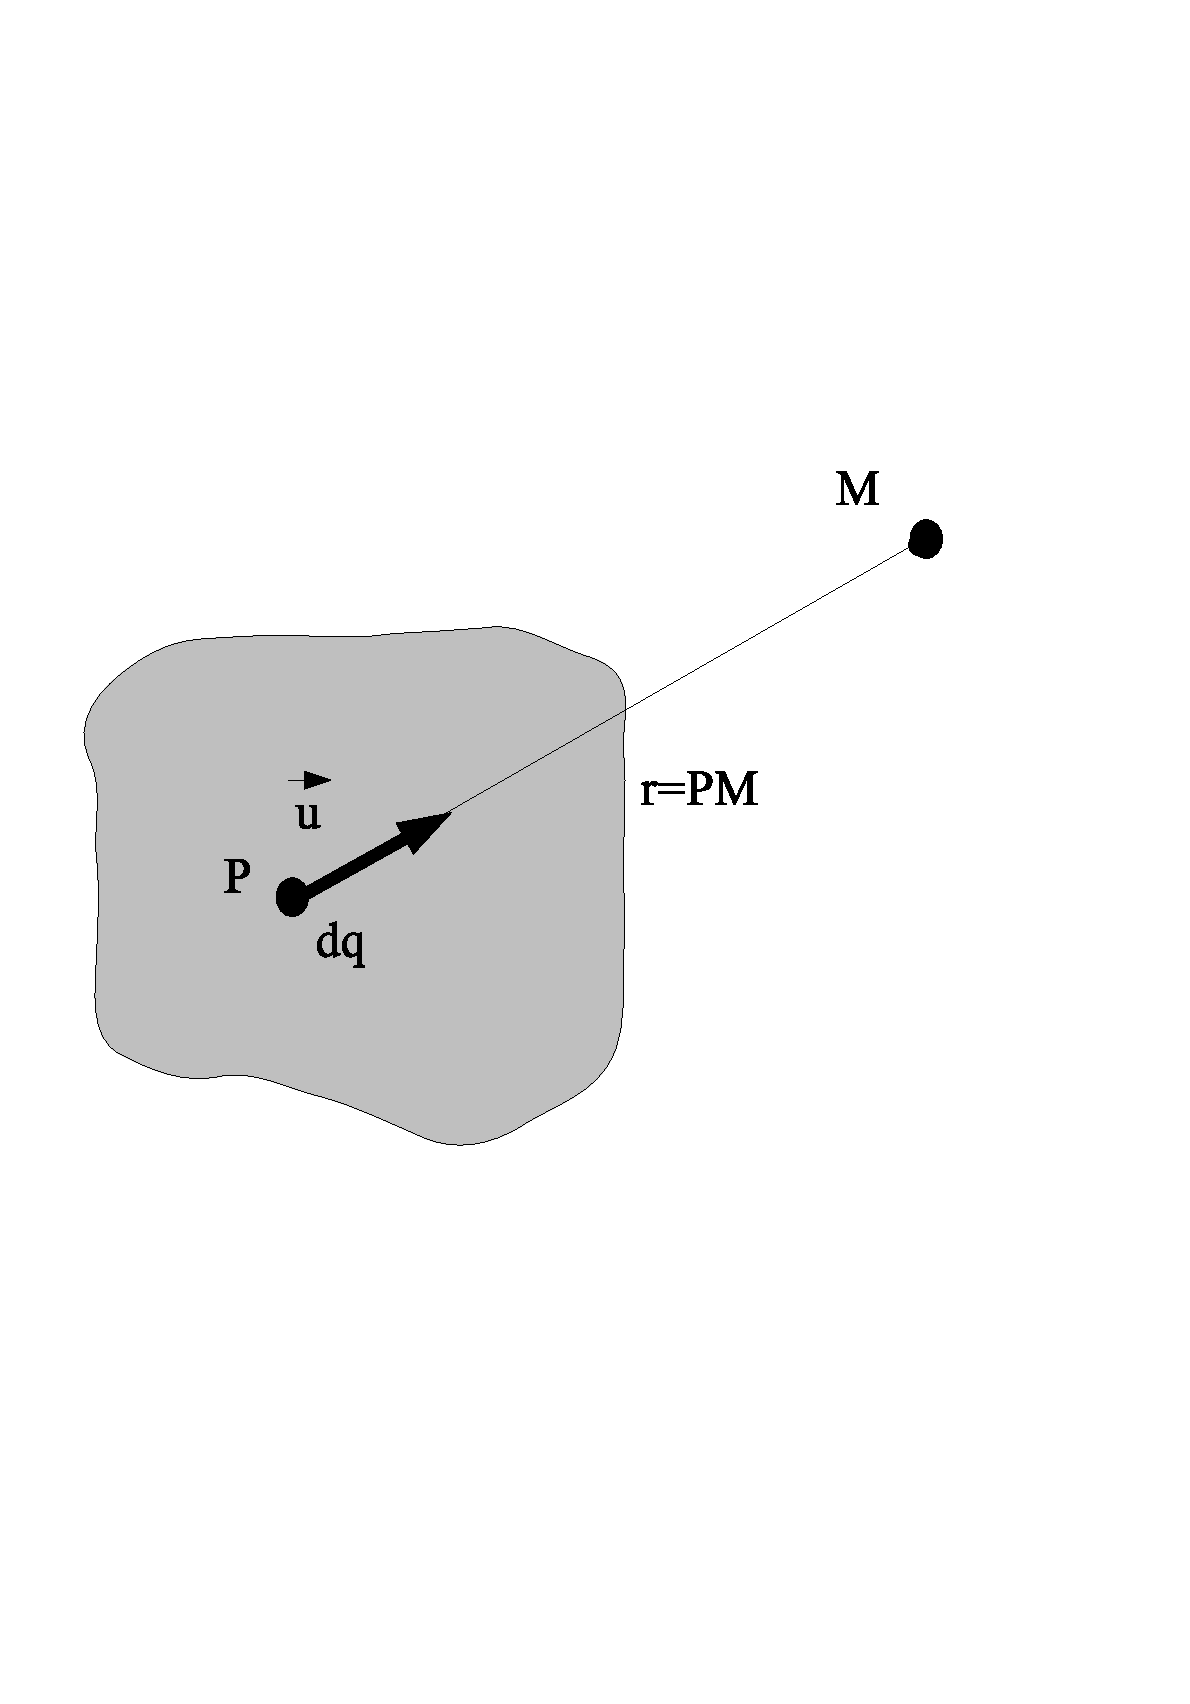
\includegraphics[clip=true,viewport=0cm 9cm 24cm 22cm,scale=0.3]{./figures/distribution_continue_de_charges.pdf}
\caption{G�om�trie du probl�me de la distribution continue de charges.}
\end{center}
\end{figure}

On d�finit $\rho =\fractext{\ud q}{\ud V}$ comme �tant la \bold{densit� volumique de charges} dans l'�l�ment de volume $\ud V$  (unit�~: $\mathrm{C.m^{-3}}$). Le champ �lectrostatique cr�� par une telle distribution dans l'ensemble du volume $V$ est donc~:

\begin{equation}
\vec{E}(M)=\iiint_{V} \frac{1}{4\pi\varepsilon_{0}}\frac{\rho}{r^{2}}\vec {u} \,\ud V.
\end{equation}

Lorsque l'une des dimensions de la distribution de charges est beaucoup plus petite que les deux autres, (ex~: un plan ou une sph�re creuse), on peut g�n�ralement faire une int�gration sur deux dimensions. On d�finit alors la \bold{densit� surfacique de charges} $\sigma  =\fractext{\ud q}{\ud S}$ dans l'�l�ment de surface $\ud S$ (unit�~: $\mathrm{C.m^{-2}}$) et le champ total sur la surface $S$ devient :

\begin{equation}
\vec{E}(M)=\iint_{S} \frac{1}{4\pi\varepsilon_{0}}\frac{\sigma}{r^{2}}\vec {u} \,\ud S.
\end{equation}

Enfin, si deux des dimensions de la distribution sont n�gligeables devant la troisi�me (ex~: un fil), on peut d�finir une \bold{densit� lin�ique de charges} $\lambda   =\fractext{\ud q}{\ud l}$ dans l'�lement de longueur $\ud l$ (unit�~: $\mathrm{C.m^{-1}}$) et le champ total sur la longueur $L$ s'�crit~:

\begin{equation}
\vec{E}(M)=\int_{L} \frac{1}{4\pi\varepsilon_{0}}\frac{\lambda}{r^{2}}\vec {u} \,\ud l.
\end{equation}

\subsection{Repr�sentation des champs}

Les �quations pr�c�dentes ont montr� qu'on peut calculer un vecteur champ �lectrique dans n'importe quel cas de distribution de charges. Pour repr�senter ce champ, on utilise les lignes de champs qui sont sont tangentes � la direction du vecteur en chaque point de l'espace. Plus le champ est fort, plus les lignes sont serr�es. De m�me, plus le champ est faible, plus les lignes sont espac�es. Les lignes de champs ne se coupent pas et partent des charges positives (ou de l'infini) pour aboutir aux charges n�gatives (ou � l'infini). On y ajoute des fl�ches pour rappeler le sens du champ comme le montre l'exemple � la figure \ref{lignes_champ}.

\begin{figure}[h]
\begin{center}
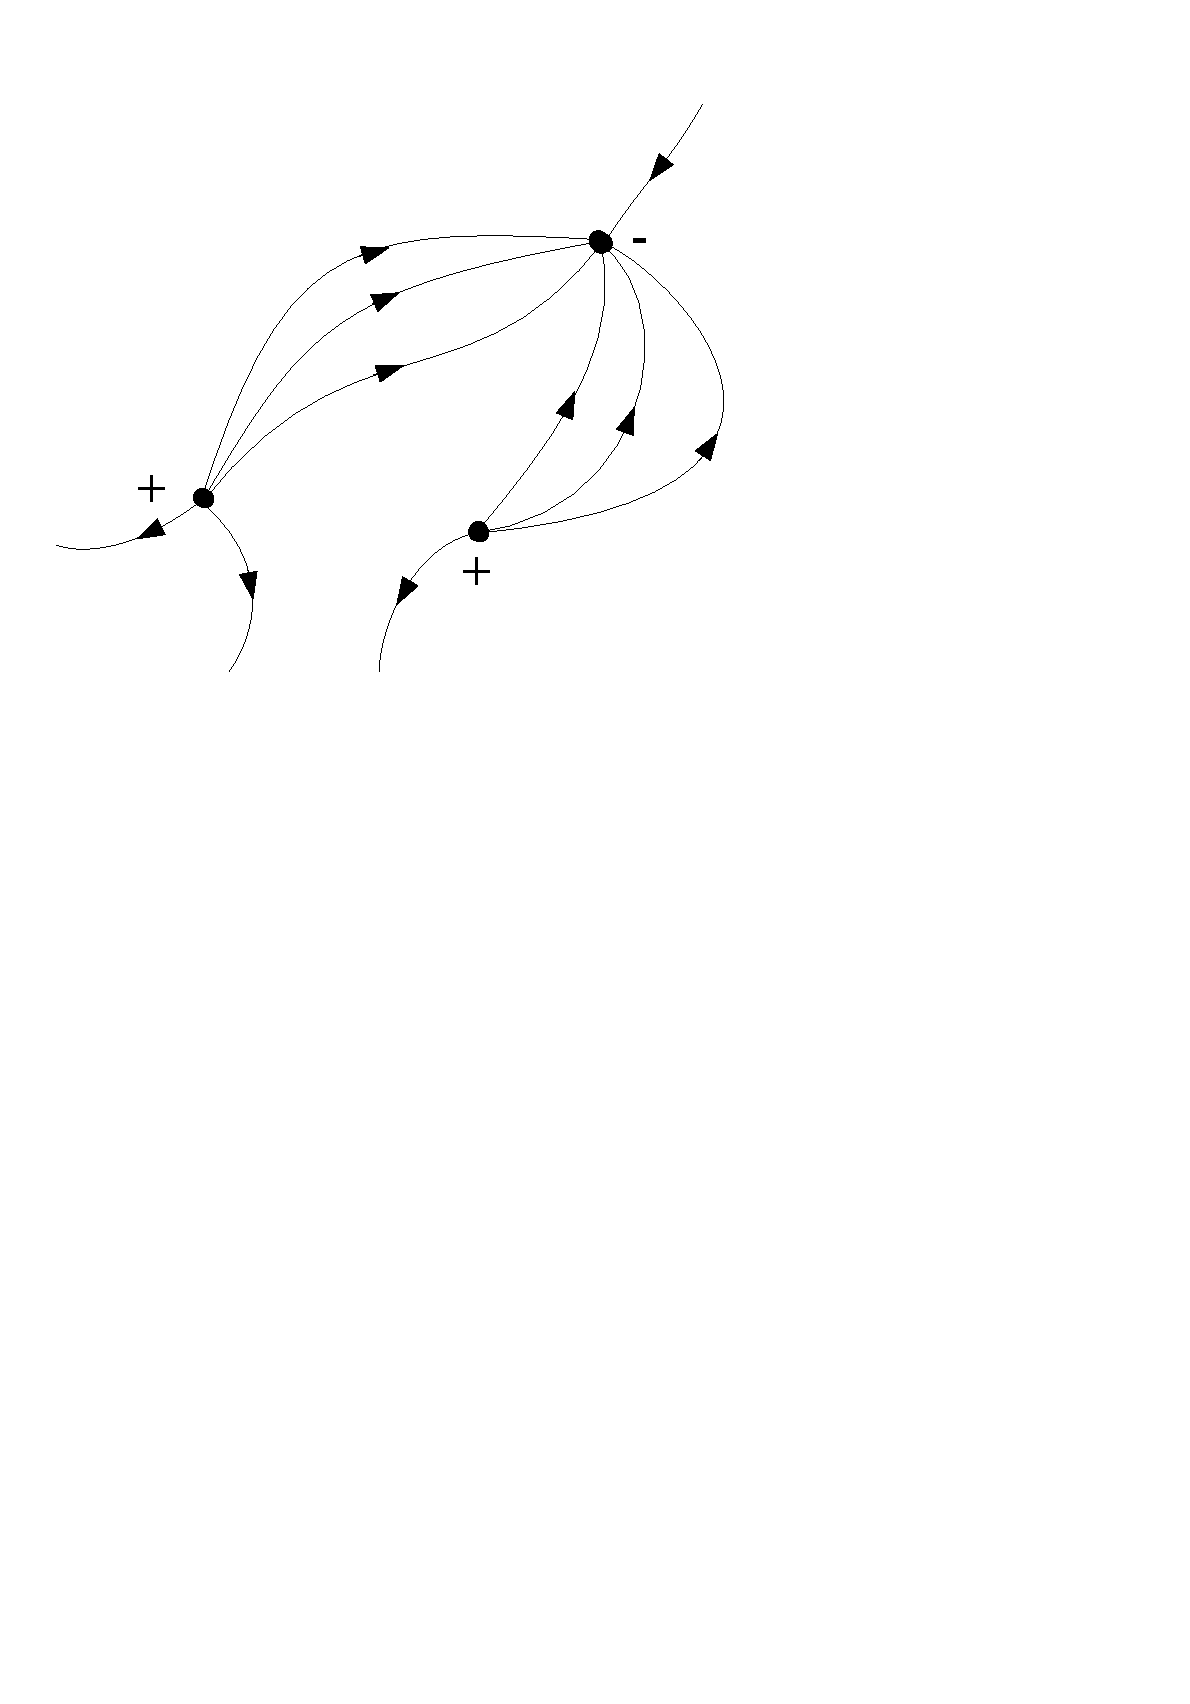
\includegraphics[clip=true,viewport=0cm 17cm 17cm 27cm,scale=0.4]{./figures/lignes_de_champ.pdf}
\caption{Exemple d'un trac� de lignes de champ entre des charges ponctuelles positives et n�gatives.}
\end{center}\label{lignes_champ}
\end{figure}


\section{Etude du champ �lectrique}

\subsection{Notion d'angle solide}
La notion d'angle solide est l'extension naturelle dans l'espace de la notion d'angle d�finie dans un plan. Dans un espace � 3 dimensions, l'oeil regarde par exemple tous les objets selon un angle solide mais ne voit finalement qu'une surface projet�e. De m�me lors d'une prise de vue photographique : pour une m�me surface de projection, l'angle r�el percu par l'objectif est variable et d�pend de sa distance focale. Dans ce cas pr�cis, plus la focale est petite, plus l'angle solide per�u est grand. C'est en modifiant cet angle solide qu'on produit l'effet << zoom >>.

\begin{figure}[h]
\begin{center}
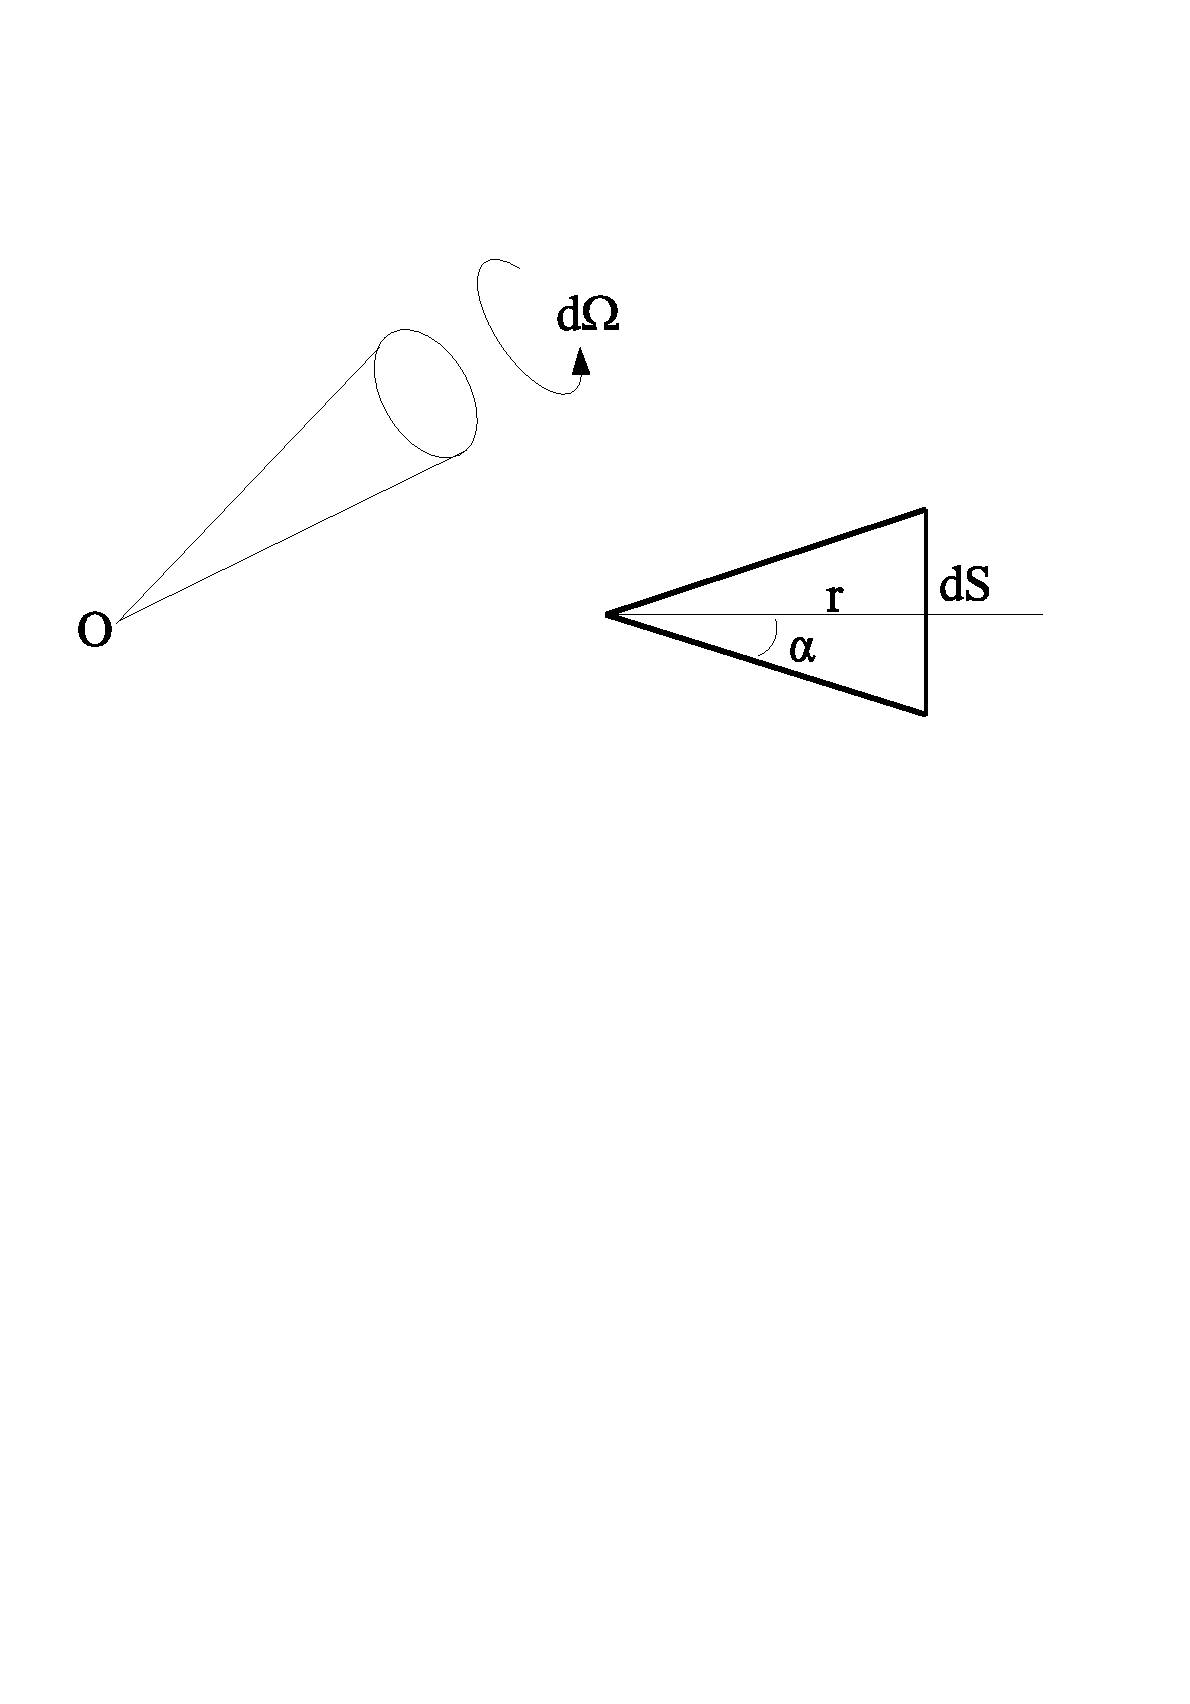
\includegraphics[clip=true,viewport=0cm 16cm 22cm 25cm,scale=0.4]{./figures/angle_solide.pdf}
\caption{Sch�ma repr�sentatif d'un angle solide.}
\end{center}
\end{figure}

\begin{defi}
L'angle solide �l�mentaire $\ud \Omega$, d�limit� par un c�ne coupant un �l�ment de surface $\ud S$ situ�e � une distance $r$ de son sommet $O$ vaut~:
\begin{equation}\label{angle_solide}
\boxed{\ud \Omega =\frac{\ud S}{r^{2}}.}
\end{equation}
Cet angle solide est toujours positif et son unit� est le `st�radian' (sr).
\end{defi}

En coordonn�es sph�riques, la surface �l�mentaire � $r$ constant vaut $\ud S=r^{2}\sin{\vartheta } \ud \vartheta \ud \varphi $. L'angle solide �l�mentaire s'�crit alors $\ud \Omega =\sin {\vartheta } \ud \vartheta  \ud \varphi$. Ainsi, l'angle solide d�limit� par un c�ne de r�volution, d'angle au sommet $\alpha $ vaut~:

\begin{equation}
	\Omega =\int \ud \Omega =\int_{0}^{2\pi } \ud \varphi \int_{0}^{\alpha } \sin{\vartheta } \ud \vartheta =2\pi (1-\cos{\alpha} ).
\end{equation}

Le demi-espace, engendr� avec $\alpha =$ \fract $\pi$/2 radians, correspond donc � un angle solide de $2\pi$ st�radians, tandis que l'espace entier correspond � un angle solide de $4\pi$ $(\alpha =\pi )$. On remarque que l'angle solide calcul� ne d�pend pas de $r$.

Dans le cas g�n�ral, le c�ne peut intercepter une surface quelconque dont la normale $\vec{n}$ fait un angle $\vartheta $ avec la g�n�ratrice de vecteur directeur $\vec{u}$. L'angle solide �l�mentaire est alors d�fini par~:

$$\ud \Omega = \frac{\vec{\ud S}\cdot \vec{u}}{r^{2}}=\frac{\ud S \, \vec {n} \cdot \vec {u}}{r^{2}}=\frac{\ud S \cos\vartheta }{r^{2}}$$

On en d�duit :

\begin{equation}
	\ud \Omega=\frac{\ud S'}{r^{2}}
\end{equation}

\noindent o� $\ud S'$ est la surface effective qui, par exemple, serait vue par un observateur situ� en $O$.


\begin{figure}[h]
\begin{center}
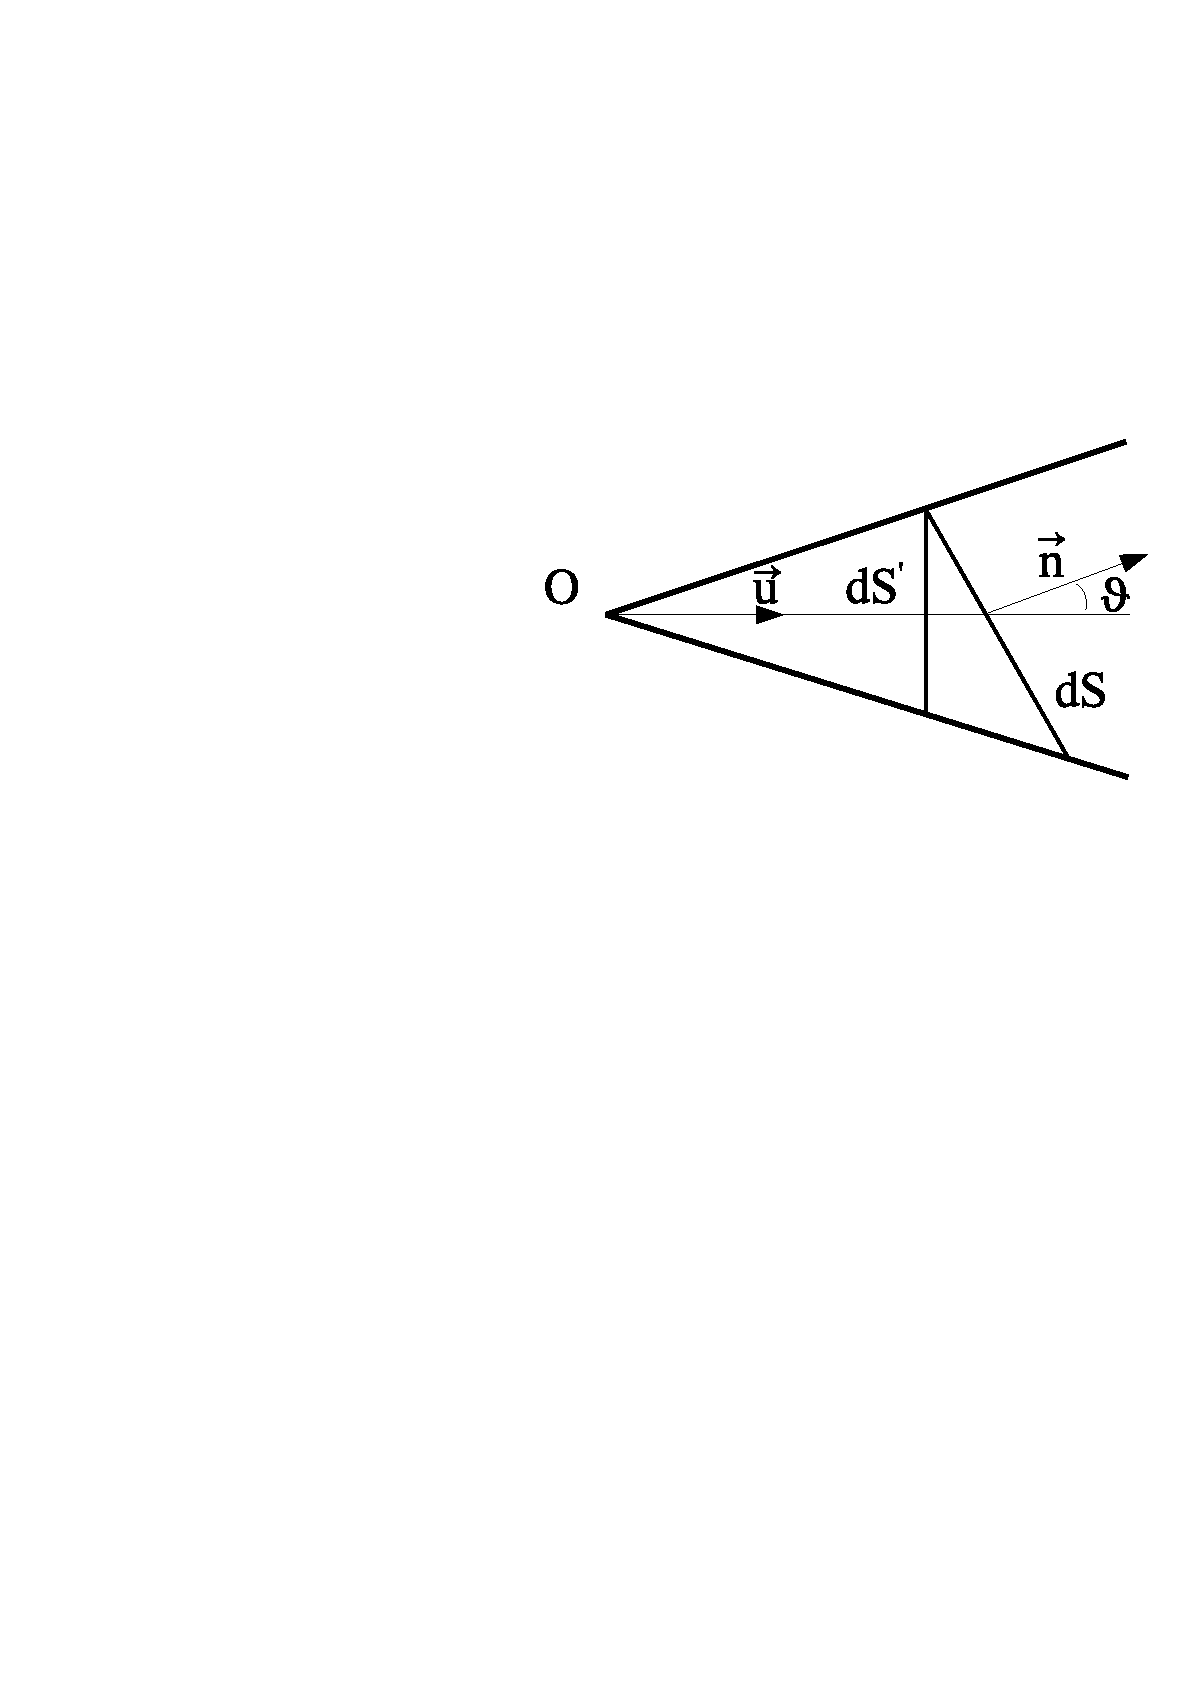
\includegraphics[clip=true,viewport=8cm 15cm 21cm 24cm,scale=0.3]{./figures/angle_solide_gene.pdf}
\caption{G�om�trie li�e au calcul d'un angle solide quelconque.}
\end{center}
\end{figure}

\subsection{Caract�risation des champs de vecteur~: le flux}
\subsubsection{A travers un �l�ment de surface}

\begin{defi}[Flux �l�mentaire]
On appelle flux �l�mentaire d'un vecteur $\vec{E}$ � travers une surface $\vec{\ud S}$ la quantit�~:
$$\ud \Phi =\vec{E} \cdot  \vec {\ud S}=E \, \ud S \, \cos{\alpha}=\frac{1}{4\pi\varepsilon_{0}}\frac{q}{r^{2}} \ud S \cos{\alpha}, $$

d'o� :

\begin{equation}
	\boxed{\ud \Phi=\frac{1}{4\pi\varepsilon_{0}}q\ \ud\Omega.}
\end{equation}
\end{defi}

\begin{rem}[Analogie]
Si le vecteur $\vec{E}$ �tait une vitesse, le flux repr�senterait un d�bit volumique.
\end{rem}

\begin{figure}[h]
\begin{center}
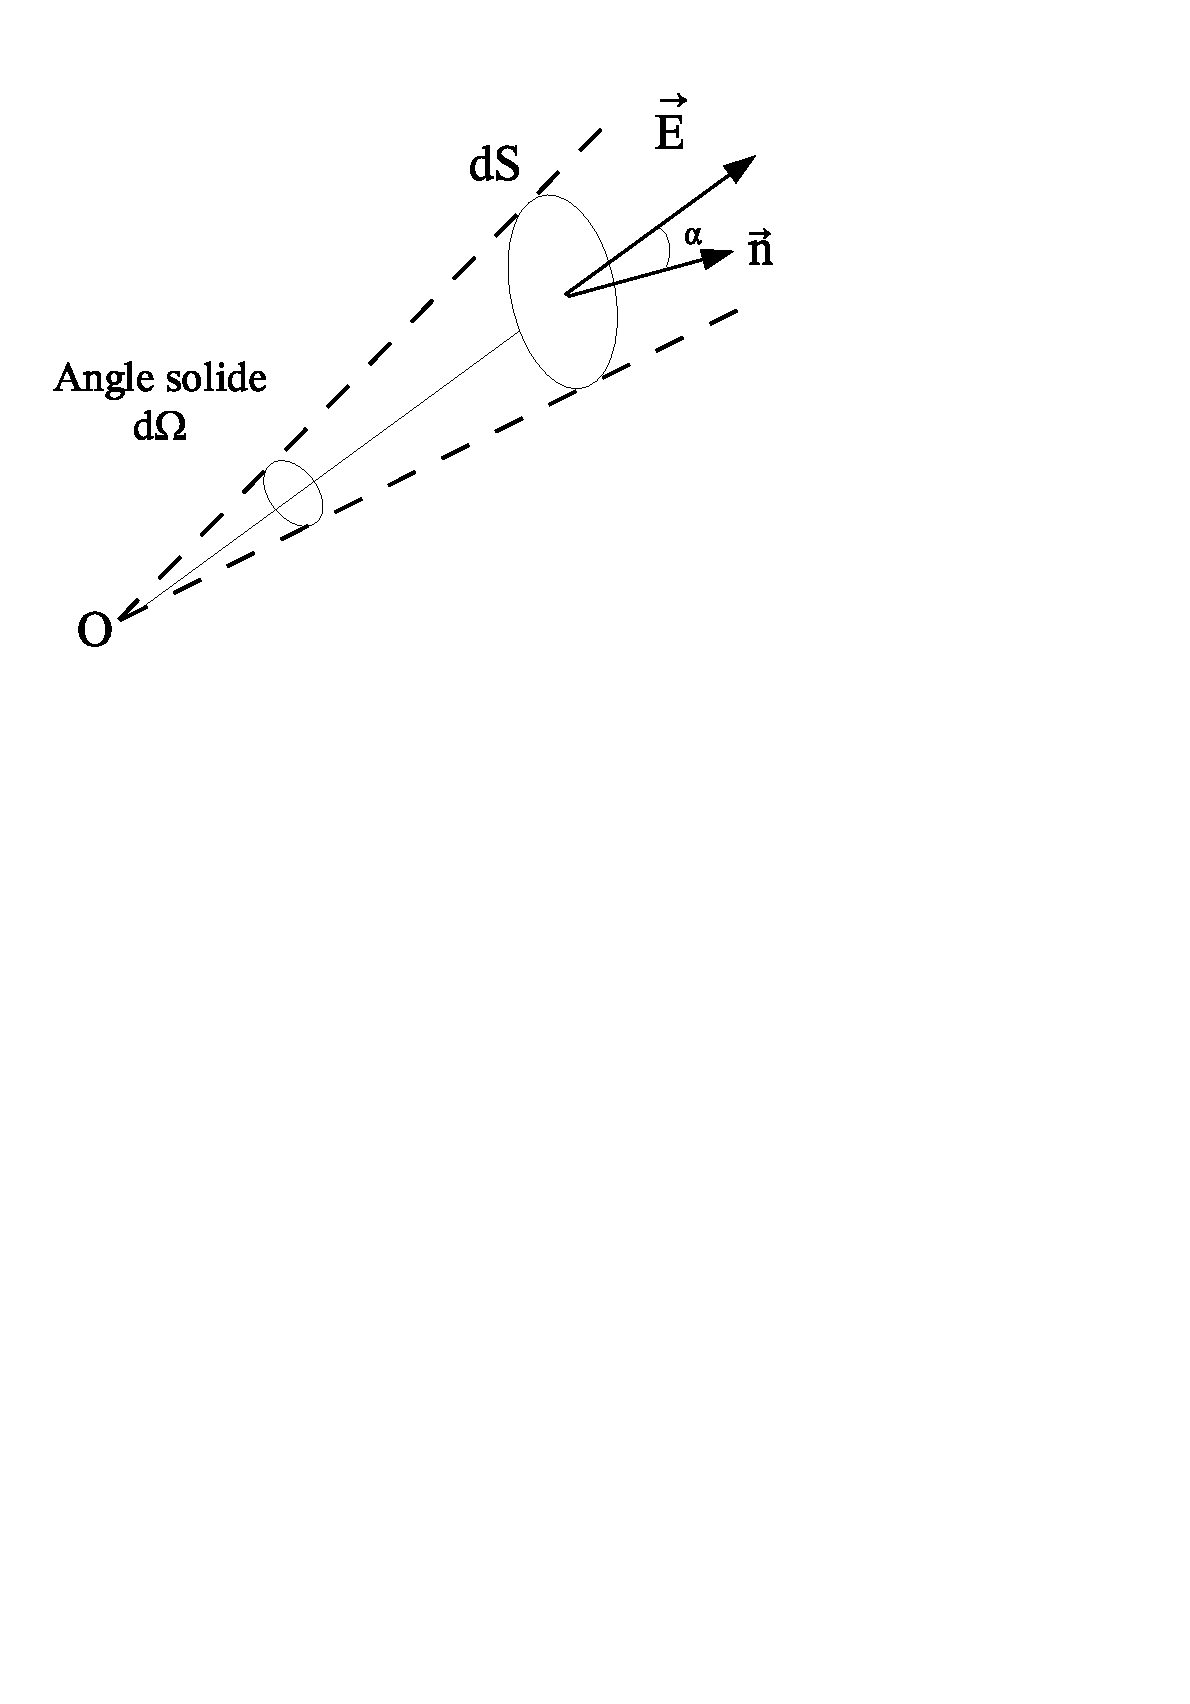
\includegraphics[clip=true,viewport=0cm 17.5cm 15cm 27.5cm,scale=0.35]{./figures/flux_elementaire.pdf}
\caption{G�om�trie pour le calcul d'un flux �l�mentaire passant � travers une surface �l�mentaire.}
\end{center}
\end{figure}

\begin{rem}[Surface orient�e]
Le signe d�pend de l'orientation de la normale \cad de $\cos \alpha$. Par la suite et par convention, nous choisirons l'orientation de $\vec{\ud S}$ dirig�e vers l'ext�rieur de la surface $S$. Ainsi, pour $q>0$, le champ $\vec{E}$ est dirig� dans le m�me sens que $\vec{n}$ et l'on obtient un flux positif.
\end{rem}

\subsubsection{Th�or�me de Gauss}

Le flux � travers une surface quelconque est �gal � la somme des flux �l�mentaires~:

\begin{equation}\label{flux_tot}
\begin{split}
\Phi = \int_{Dist.} \ud \Phi & =\iint_{S} \vec{E} \cdot \vec{\ud S} \\
& = \iint_{S} \frac{1}{4\pi\varepsilon_{0}} q \, \ud \Omega
\end{split}
\end{equation}

Prenons une charge $q$ � l'int�rieur d'une surface ferm�e.

\begin{figure}[h]
\begin{center}
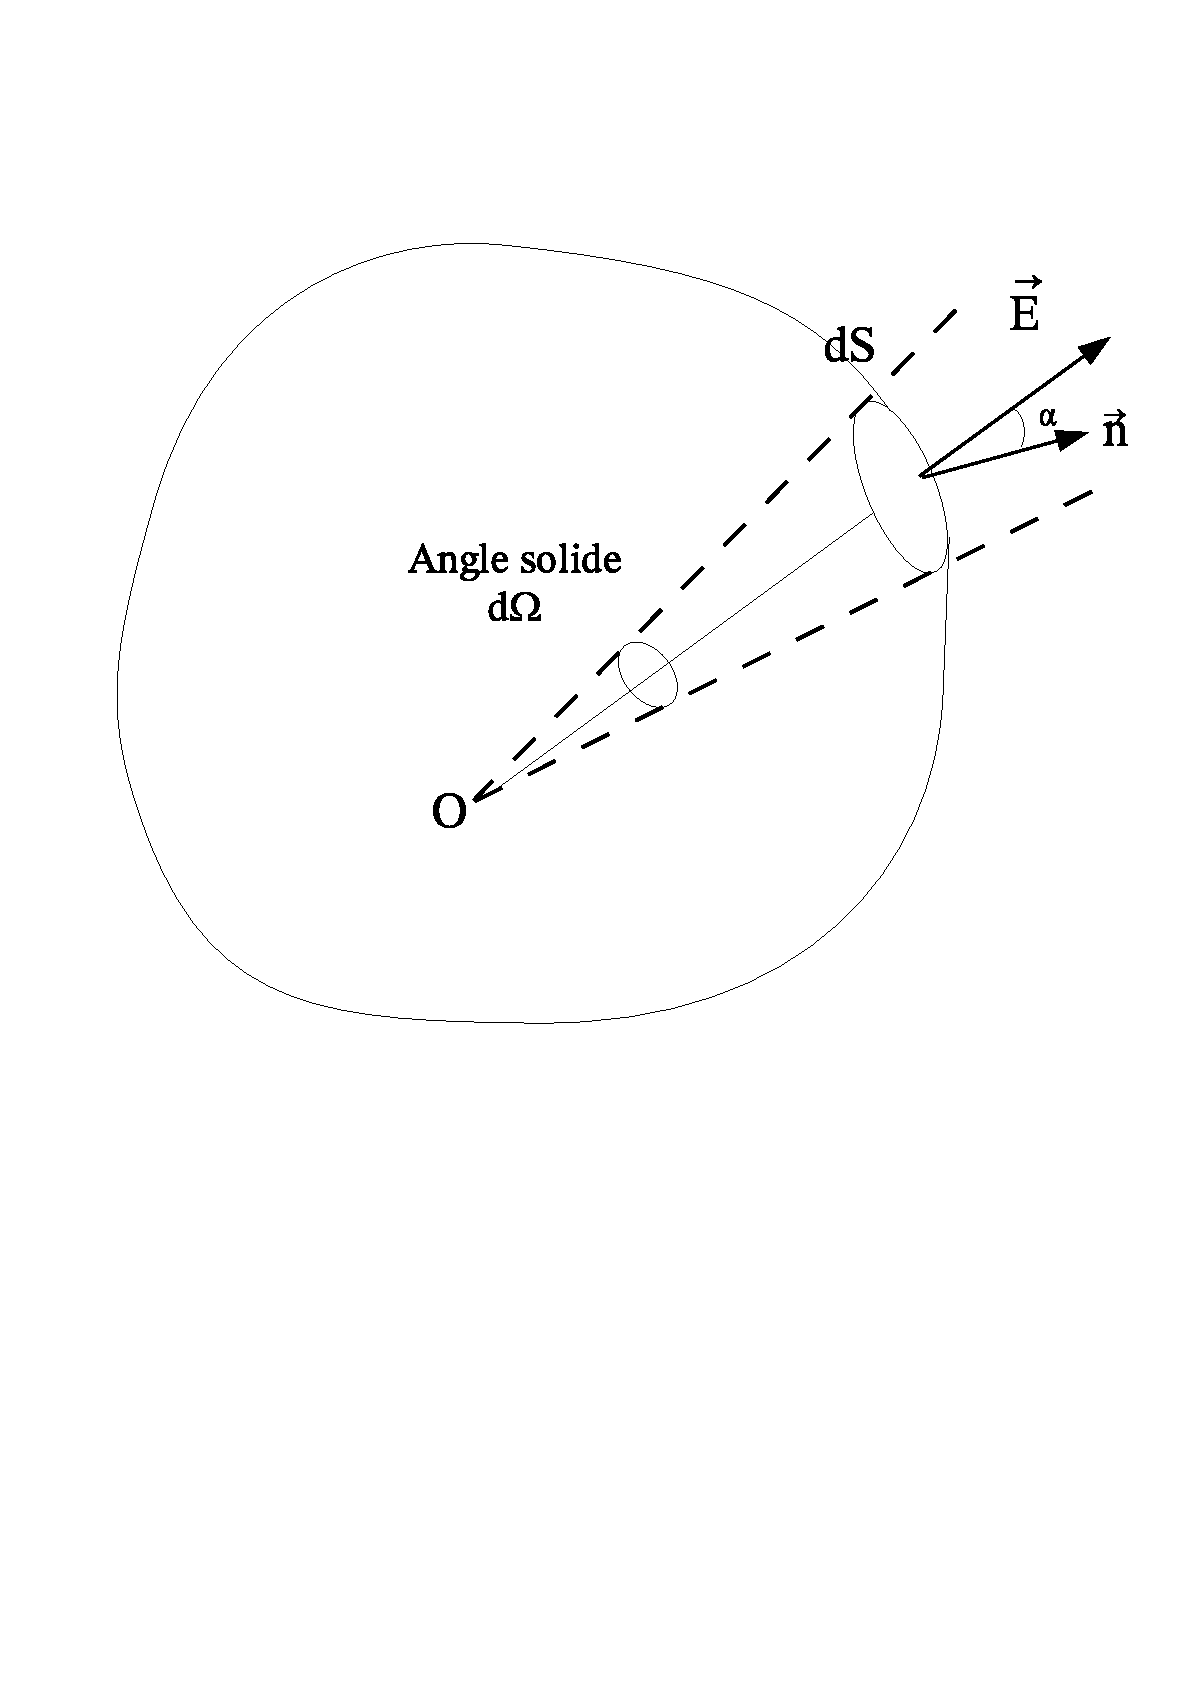
\includegraphics[clip=true,viewport=0cm 11cm 20cm 25cm,scale=0.38]{./figures/flux_surface.pdf}
\caption{Flux � travers une surface.}
\end{center}
\end{figure}


En int�grant l'�quation \ref{flux_tot} selon toutes les directions (c'est-�-dire sur les $4\pi$ st�radians), on obtient le flux total suivant:

$$\Phi = \frac{q}{\varepsilon_{0}}$$

En vertu du principe de superposition, ce r�sultat se g�n�ralise ais�ment � un ensemble quelconque de charges.

\begin{defi}[Th�or�me de Gauss]
Le flux du champ �lectrique � travers une surface ferm�e orient�e quelconque est �gal au produit de la charge �lectrique contenue � l'int�rieur de cette surface et de la constante $1/ \varepsilon_{0}$:
\begin{equation}\label{gauss}
 \boxed{\Phi = \iint_{S} \vec{E} \cdot \vec{\ud S} = \frac{Q_{int}}{\varepsilon_{0}}}
\end{equation}
\end{defi}


\subsection{Applications}

Le th�or�me de Gauss fournit une m�thode tr�s utile et performante pour calculer le champ $\vec{E}$ lorsque celui-ci poss�de des propri�t�s particuli�res de sym�trie. Celles-ci permettent en effet de simplifier le calcul du flux $\Phi $. Comme le th�or�me de Gauss est valable sur une surface quelconque, il nous suffit de trouver une surface $S$ adapt�e, c'est-�-dire respectant les propri�t�s de sym�trie du champ, appel�e \textbf{surface de Gauss}.

\begin{bex}[Champ au voisinage d'un fil infiniement mince, uniform�ment charg�]
A voir en TD
\end{bex}

\begin{bex}[Champ au voisinage d'une plaque infinie, uniform�ment charg�e]
A voir en TD
\end{bex}

\begin{bex}[Champ au voisinage d'une boule uniform�ment charg�e de rayon $R$]
A voir en TD
\end{bex}


\section{Potentiel}

\subsection{Notion de potentiel �lectrostatique}

Nous avons vu qu'il fallait calculer 3 composantes pour obtenir $\vec{E}$. Ces composantes peuvent �tre d�duites d'un champ potentiel, \cad scalaire, � l'aide de la fonction vectorielle nomm�e \textbf{gradient} :


\begin{defi}
 Soit $\vec{E}$ un champ �lectrostatique quelconque. $\vec{E}$ d�rive du potentiel �lectrostatique $V$ tel que:
\begin{equation}
\vec{E}=-\grad\ V
\end{equation}
\end{defi}

\begin{note}[Historique]
En fait, depuis Newton (1687) et sa loi de gravitation universelle, de nombreux physiciens et math�maticiens s'�taient pench�s sur les propri�t�s de cette force radiale en 1/$r^{2}$. En particulier Lagrange avait introduit en 1777 une fonction scalaire appel�e `potentiel', plus fondamentale puisque la force en d�rive. C'est Poisson qui introduit le potentiel �lectrostatique en 1813, par analogie avec la loi de Newton.
\end{note}

\begin{note} Le signe moins est une convention li�e � celle adopt�e pour l'�nergie �lectrostatique.
\end{note}

\subsection{Vecteur Gradient}

Soit $V(M)$ un scalaire d�fini en tout point $M$ de l'espace, \cad un \textbf{champ scalaire}. Lorsqu'on passe d'un point $M$ � un point $M'$ infiniment proche, une variation $\ud V$ de ce champ est alors fourni par la diff�rentielle totale suivante~:

$$\ud V(M)=\sum_{i=1}^{3}\frac{\partial V}{\partial x_{i}} \ud x_{i}= \grad\ V \cdot \ud \overrightarrow{OM}$$

\noindent o� le vecteur $\grad\ V$ est le gradient du champ scalaire V et constitue un champ de vecteurs d�fini partout. Ses composantes dans un syst�me de coordonn�es donn� sont obtenues tr�s simplement. Par exemple, en coordonn�es cart�siennes, on a $\overrightarrow{\ud OM} = \ud x \, \vec{i} +  \ud y \, \vec{j} +  \ud z \, \vec{k}$ et~:

$$\ud V = \frac{\partial V}{\partial x} \, \ud x + \frac{\partial V}{\partial y} \, \ud y +\frac{\partial V}{\partial z} \, \ud z $$

\noindent d'o� l'expression suivante pour le gradient en coordonn�es cart�siennes~:

\begin{equation}\label{grad}
\grad\ V =
			\begin{pmatrix} \cfrac{\partial V}{\partial x} \\
							\\
							\cfrac{\partial V}{\partial y} \\
							\\
							\cfrac{\partial V}{\partial z}
			\end{pmatrix}
\end{equation}

En faisant de m�me en coordonn�es cylindriques et sph�riques, on obtient respectivement~:

$$
\grad\ V =
			\begin{pmatrix} \cfrac{\partial V}{\partial \rho } \\
							\\
							\cfrac{1}{\rho }\cfrac{\partial V}{\partial \vartheta } \\
							\\
							\cfrac{\partial V}{\partial z}
			\end{pmatrix}
\qquad \textrm{et} \qquad
\grad\ V =
			\begin{pmatrix} \cfrac{\partial V}{\partial r} \\
							\\
							\cfrac{1}{r} \cfrac{\partial V}{\partial \vartheta} \\
							\\
							\cfrac{1}{r \sin{\vartheta }}\cfrac{\partial V}{\partial \varphi }
			\end{pmatrix}
.$$

\subsection{Circulation du vecteur $\vec{E}$}

Le potentiel est li� au travail accompli pour transf�rer une charge d'un point � un autre. De mani�re analogue au travail d'une force, on d�finit la circulation $\mathcal{C}$ de $\vec{E}$ le long de la courbe $(AB)$ par l'�quation :

$$ \mathcal{C}=\int_{A}^{B} \vec{E} \cdot \vec{\ud l}$$

Ainsi,

\begin{equation*}
\begin{split}
\mathcal{C} & =\int_{A}^{B} \frac{q}{4 \pi \varepsilon_{0}} \frac{\vec{\ud l} \cdot \vec{u}}{r^{2}} \\
& =\int_{A}^{B} \frac{q}{4 \pi \varepsilon_{0}} \frac{\ud r}{r^{2}} \\
& = - \frac{q}{4 \pi \varepsilon_{0}} \biggl[ \frac{1}{r} \biggr]_{A}^{B} \\
& = \frac{q}{4 \pi \varepsilon_{0}r_{A}} - \frac{q}{4 \pi \varepsilon_{0}r_{B}} \\
& = V_{A} - V_{B}
\end{split}
\end{equation*}


\begin{figure}[h]
\begin{center}
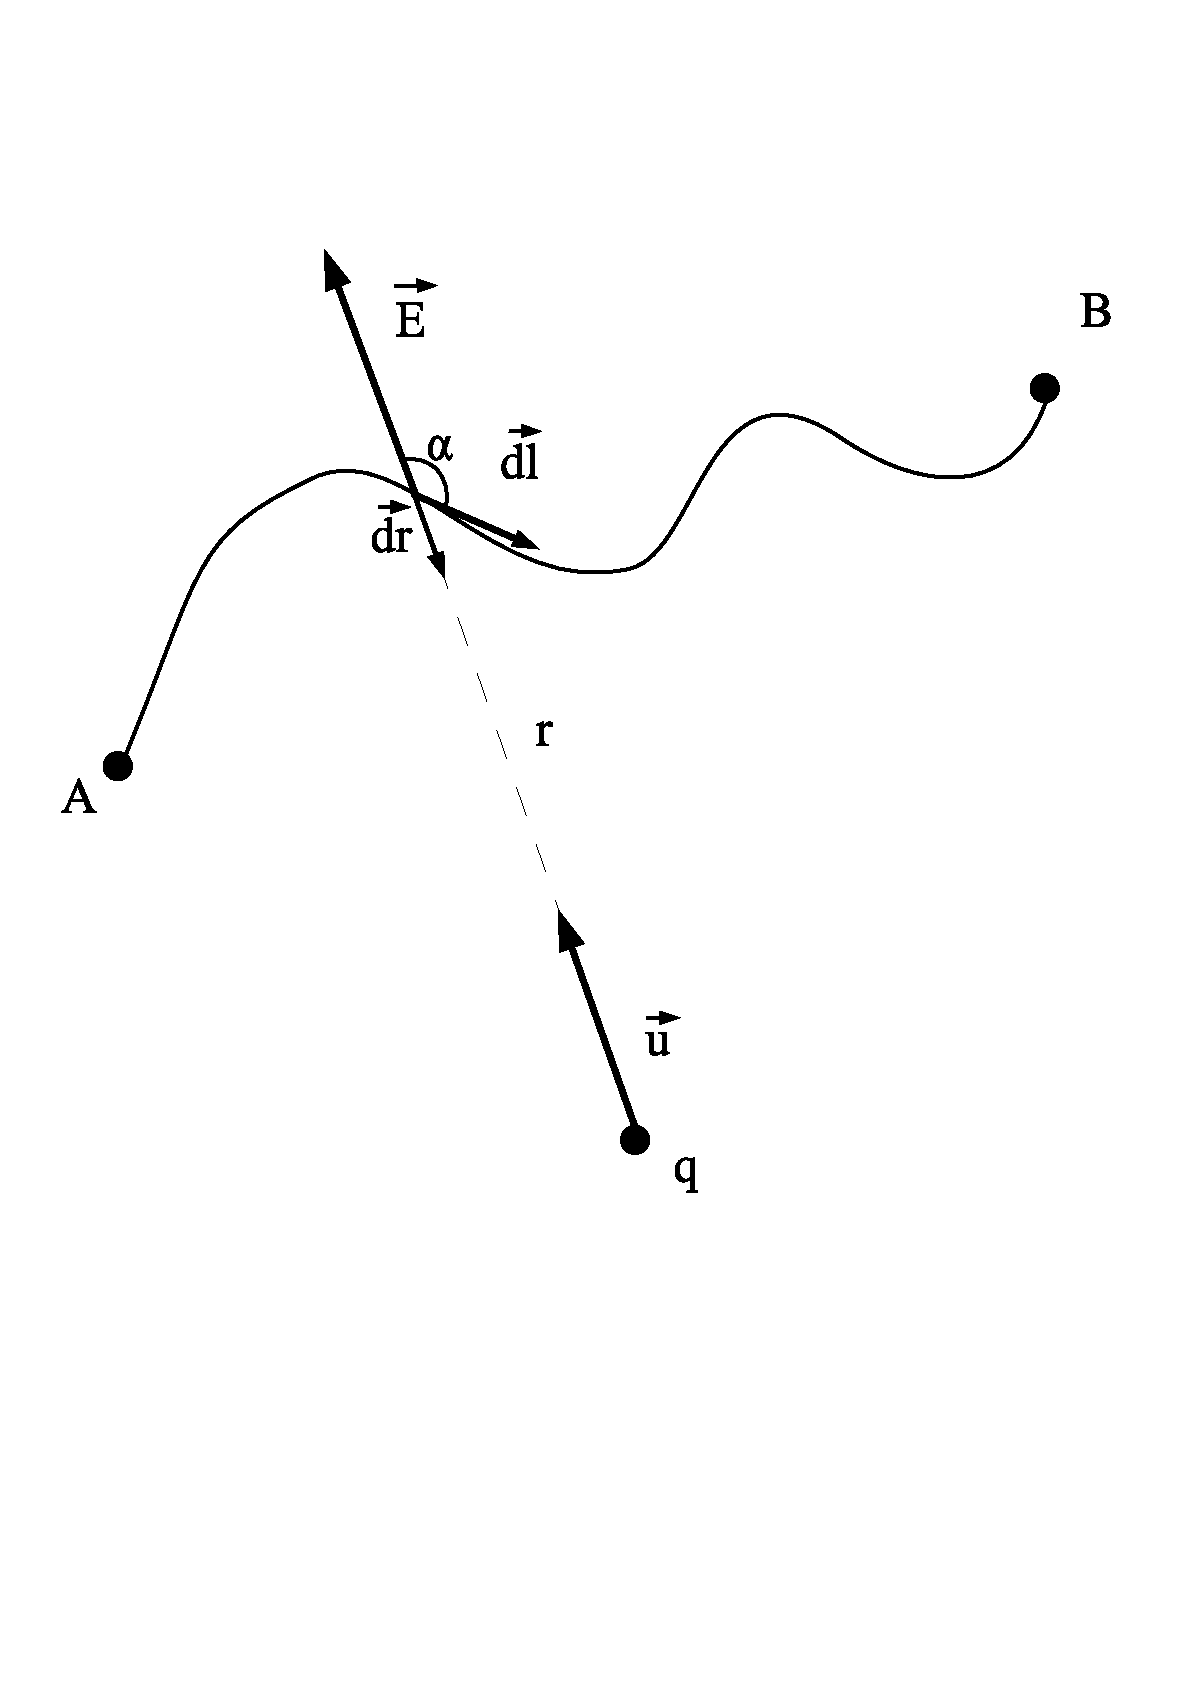
\includegraphics[clip=true,viewport=0cm 8cm 19cm 25cm,scale=0.38]{./figures/circulation.pdf}
\caption{Calcul de la circulation entre le point A et B.}
\end{center}
\end{figure}

\begin{brems}
\mbox{}
\begin{itemize}
\item La circulation de $\vec{E}$ le long de AB ne d�pend pas de la trajectoire, mais d'une diff�rence de potentiel;
\item la circulation de $\vec{E}$ sur une courbe ferm�e est nulle.
\end{itemize}
\end{brems}


\subsection{Potentiel cr�� par une charge ponctuelle}

Consid�rons une charge ponctuelle $q$ situ�e en un point $O$. En tout point $M$ de l'espace, cette charge cr�e un champ �lectrostatique $\vec{E}$ et le potentiel �lectrostatique s'�crit~:

$$\ud V(M)=- \vec{E} \cdot \overrightarrow{\ud l}=- \frac{q}{4 \pi \varepsilon_{0}} \frac{\vec{u}\cdot \vec{\ud r}}{r^{2}}$$

On en d�duit :

\begin{equation}
\boxed{\ud V(M)=-\frac{q}{4 \pi \varepsilon_{0}} \frac{\ud r}{r^{2}}}
\end{equation}

En int�grant selon $r$ et en posant $V_0$ comme la charge le potentiel cr�� par la charge en $O$, on obtient:

\begin{equation}
V(M) = \frac{1}{4 \pi \varepsilon_{0}} \frac{q}{r} + V_{0}
\end{equation}

\begin{conventions}
\mbox{}
\begin{itemize}
\item La constante d'int�gration est g�n�ralement choisie nulle (le potentiel s'annule � l'infini) ;
\item V est un scalaire exprim� en Volt (V) ;
\item V cro�t des charges $(-)$ aux charges $(+)$ (sens de croissance de V oppos� � $\vec{E}$) ;
\item Les surfaces de potentiel constant sont appel�es �quipotentielles ;
\end{itemize}
\end{conventions}

\subsection{Potentiel cr�� par un ensemble de charges (principe de superposition)}

Nous avons vu dans le chapitre pr�c�dent que le champ �lectrique cr�� par une distribution de charges �tait �gal � la somme vectorielle des champs �lectriques cr��s par chacune de ces charges. De m�me, le potentiel �lectrique cr�� par une distribution de charges est �gal � la somme alg�brique des potentiels �lectriques cr��s par chacune de ces charges. Cette propri�t� d�coule de la propri�t� de d�rivation d'une somme qui est simplement �gale � la somme des d�riv�es. En utilisant l'expression du potentiel cr�� par une charge unique, on a ainsi~:

\begin{equation}
 \boxed{V(M) = \sum_{i=1}^{n} \frac{1}{4 \pi \varepsilon_{0}} \frac{q_i}{r_i}}
\end{equation}

\noindent o� $r_{i}$ est la distance entre la charge $q_{i}$ et le point $M$.

Lorsque l'on s'int�resse � des �chelles spatiales qui sont tr�s grandes par rapport aux distances entre les charges $q_{i}$, on peut faire un passage � la limite continue et remplacer la somme discr�te par une int�grale o� $P$ est un point courant autour duquel se trouve une charge �l�mentaire $\ud q$. Le potentiel �lectrostatique cr�� par une distribution de charges continue devient alors~:

\begin{equation}
\boxed{V(M) = \frac{1}{4 \pi \varepsilon_{0}} \int_{Dist.} \frac{\ud q} {r}}
\end{equation}

\noindent o� $r = PM$ est la distance entre le point $M$ et un point $P$ quelconque de la distribution de charges.

Pour des distributions de charges lin�iques $\lambda $, surfacique $\sigma $ et volumique $\rho$, on obtient respectivement~:

$$V(M) = \frac{1}{4 \pi \varepsilon_{0}} \int_{a}^{b} \frac{\lambda \ud l} {r}$$

$$V(M) = \frac{1}{4 \pi \varepsilon_{0}} \int_{S} \frac{\sigma  \ud S} {r}$$

$$V(M) = \frac{1}{4 \pi \varepsilon_{0}} \int_{V} \frac{\rho \ud V} {r}$$

\begin{brems}
\mbox{}
\begin{itemize}
\item Le calcul de $V$ n'implique qu'une seule int�grale alors que $\vec{E}$, en tant que vecteur, en implique plusieurs : celles des composantes. Mais, par d�finition, un scalaire ne donne pas la m�me information qu'un vecteur. En effet, la connaissance du potentiel en un point $r$ de l'espace ne permet pas de d�terminer � lui seul la force qui s'applique sur la charge $q$. Il est �galement n�cessaire de savoir comment $V$ varie au voisinage de ce point, puisque que c'est � partir des d�riv�es partielles de $V$ que seront d�duites les composantes de $\vec{E}$ et de la force.
\item Les champs et potentiels �lectriques ont �t� exprim�s dans le cas o� les charges sont dans le \emph{vide}. On a utilis�e la constante $\varepsilon_{0}$ qui est la permittivit� du vide. Dans le cas o� un mat�riau remplace le vide, on doit remplacer $\varepsilon_{0}$ par $\varepsilon$ qui est la permittivit� du mat�riau et qui peut �tre d�fini ainsi :

\begin{equation}
	\boxed{\varepsilon = \varepsilon_0 * \varepsilon_R}
\end{equation}

\noindent o� $\varepsilon_R$ est la \textbf{permittivit� relative} ou \textbf{constante di�lectrique}. Le tableau \ref{tab_epsilonR} donne les valeurs de $\varepsilon_R$ pour quelques mat�riaux.

\begin{table}
				\begin{center}
				\begin{tabular}{|c|c|} \hline
				Mat�riau & Permittivit� relative $\varepsilon_R$ \\ \hline \hline
				Vide & 1 (par d�finition) 	\\ \hline
				Air & 1,0005  \\ \hline
				Papier & 2  \\ \hline
				Polyester 	& 3,3 \\ \hline
				Teflon &2,1 \\ \hline
				PVC &	5 \\ \hline
				Verre &	5 \\ \hline
				Bak�lite &	6 \\ \hline
				Chlorure de sodium & 	6.12 \\ \hline
				Titanate de baryum &	� peu pr�s 1500 \\ \hline
				\end{tabular}
				\end{center}
				\caption{Permittivit� relative $\varepsilon_R$ de certains mat�riaux.}\label{tab_epsilonR}
\end{table}

\end{itemize}
\end{brems}

\begin{bnote}[Cartographie]
Si la topologie d'un champ vectoriel est donn�e par les lignes de champ, la topologie d'un champ scalaire est donn�e par des courbes de niveau. Nous avons vu que dans le cas d'un potentiel �lectrique, les courbes de niveau s'appellent les \textbf{�quipotentielles}. Elles joignent les points de m�me potentiel et ont les propri�t�s suivantes:\\.

\begin{itemize}
\item les �quipotentielles sont des lignes ferm�es ;
\item elles entourent les charges ;
\item le long d'une courbe d�finie par $V=cste$ correspond � $\ud V = 0$, ce qui signifie que $\grad V$ est un vecteur perpendiculaire en tout point � cette courbe (ligne ou surface).\\
\end{itemize}

On peut effectuer une analogie avec les cartographies o� le relief est repr�sent� par des courbes de niveaux. Ces lignes rejoignent les points situ�s � la m�me altitude, \cad les points de m�me �nergie potentielle (cf. l'�quation $E_p=\rho g h$). Ce sont des lignes ferm�es entourant les sommets et les fonds. Elles sont strictement �quivalentes aux �quipotentielles.

Les lignes �quivalentes aux lignes de champ ne sont pas repr�sent�es. Pour ce faire, il faut prendre en chaque point la perpendiculaire aux lignes de niveau. Les nouvelles lignes indiquent la direction de la pente au point consid�r� (sens de l'�coulement de l'eau). Plus les lignes de niveau sont serr�es, plus la pente est importante. La pente locale est le pendant du champ �lectrique.

\end{bnote}

\begin{figure}[h]
\begin{center}
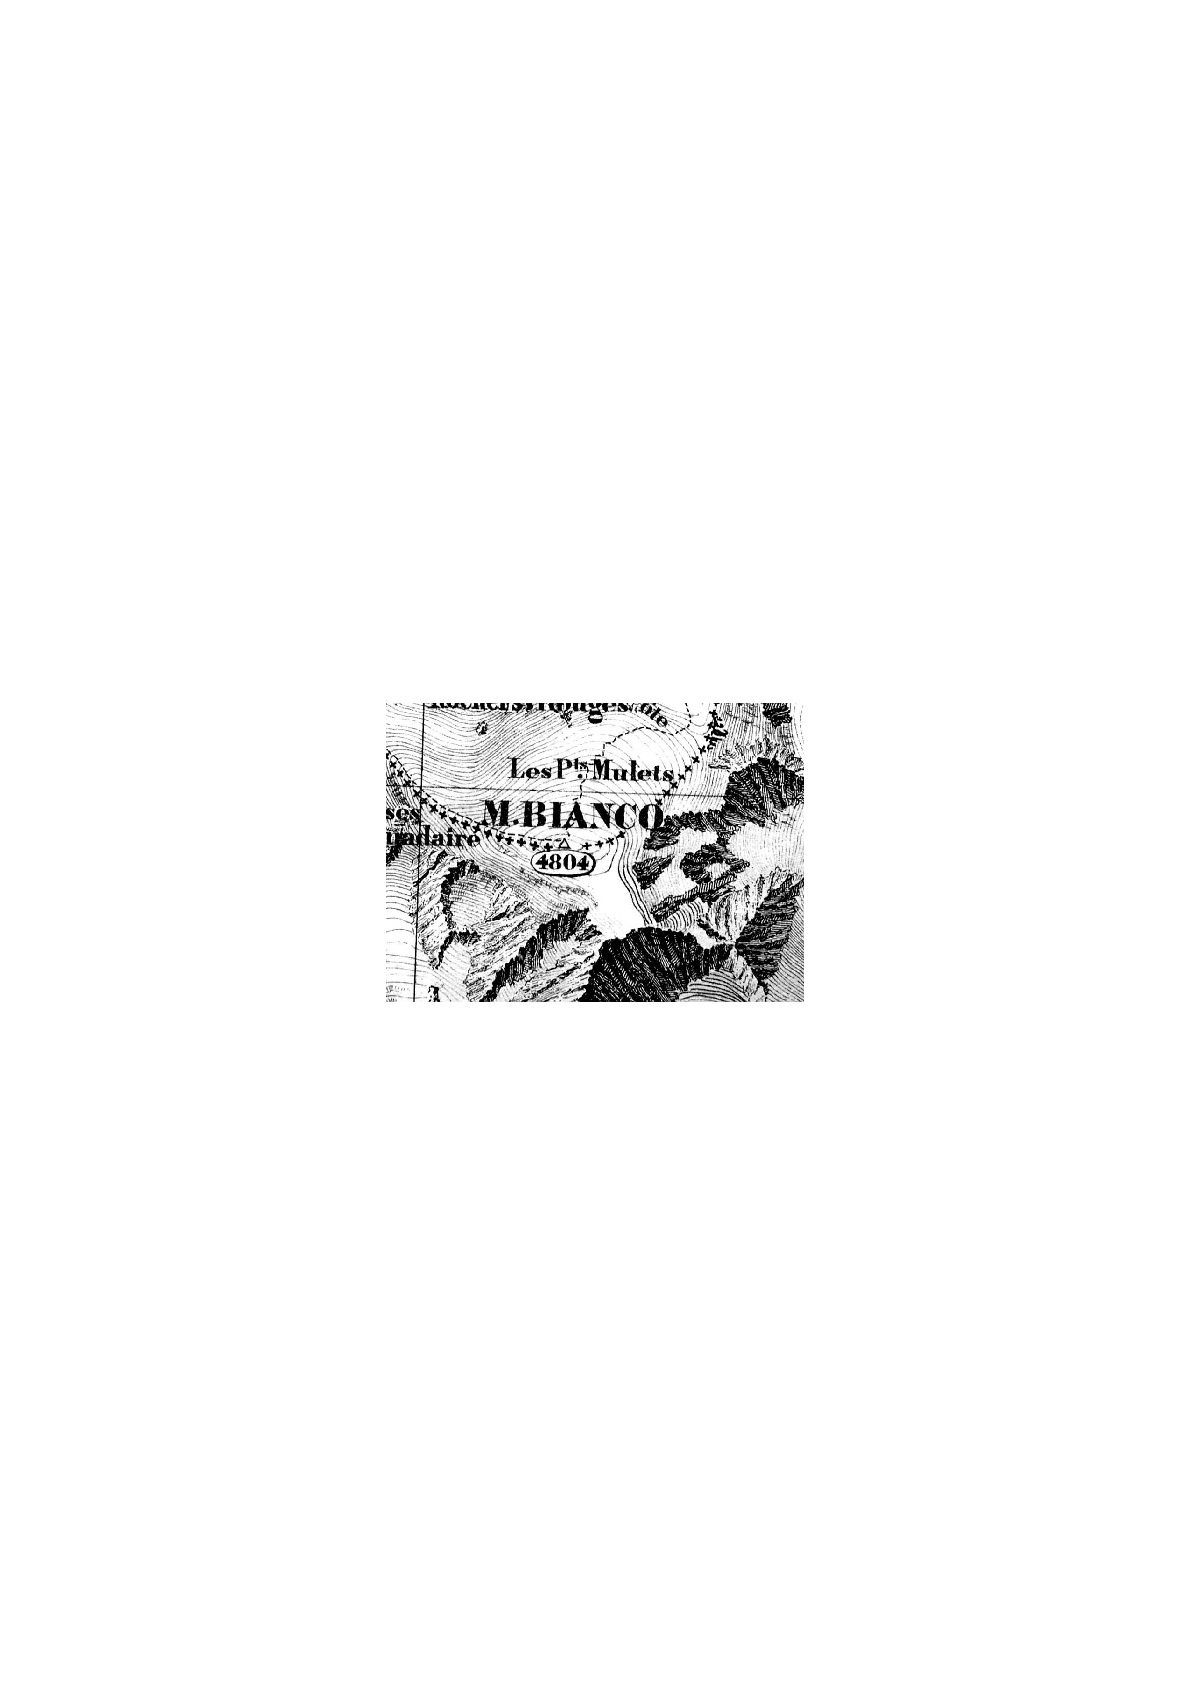
\includegraphics[clip=true,viewport=6.5cm 12cm 13.5cm 17cm,scale=1.1]{./figures/Mbianco.pdf}
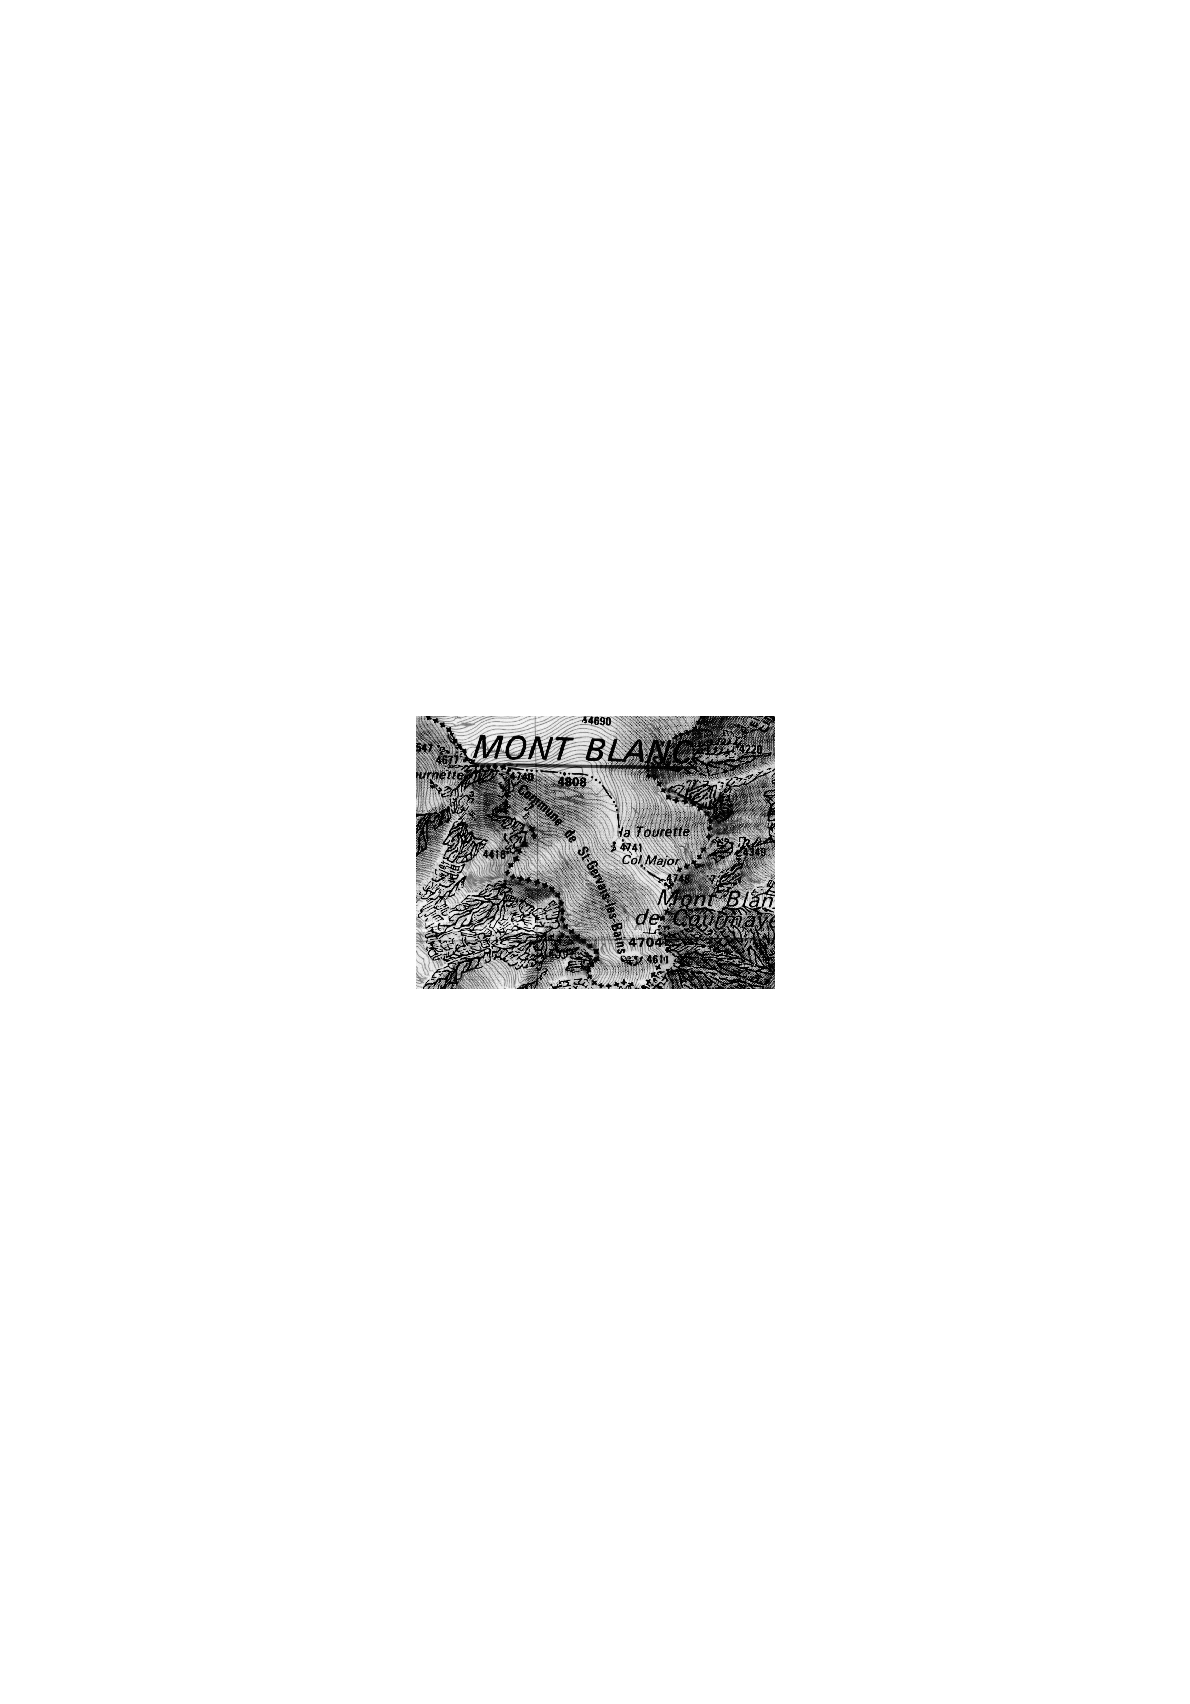
\includegraphics[clip=true,viewport=7cm 12.5cm 13cm 17cm,scale=1.28]{./figures/Mblancign.pdf}
\caption{Cartographie du mont Blanc (Extraits de la planche de l'Atlas sarde (1854) et IGN TOP 25 3531).}
\end{center}
\end{figure}


\section{Le condensateur}

\subsection{Charge des conducteurs en �quilibre}

Comme il a �t� vu pr�cedemment, la mati�re est compos�e de charges positives, les protons, localis�s dans les noyaux des atomes et de charges n�gatives, les �lectrons formant le \textbf{nuage �lectronique} dont l'extention spatial repr�sente la taille de l'atome. Les �lectrons peuvent �tre class�s en deux groupes : les �lectrons de couches profondes qui sont fortement li�s aux noyaux et les �lectrons des couches p�riph�riques qui peuvent passer d'un atome � l'autre. Ils �tablissent ainsi la liaison chimique et assurent la stabilit� des mol�cules ou des solides.

Dans les conducteurs, les �lectrons sont libres de se d�placer dans l'ensemble du mat�riau. Les �lectrons lib�r�s par les atomes sont appel�s les �lectrons libres. La \textbf{valence} d'un m�tal est �gale au nombre d'�lectrons que lib�re chacun des atomes. En l'absence de sollicitation �lectrique ext�rieure, un m�tal est �lectriquement neutre en chacun de ses points (petit volume l�g�rement sup�rieur � la taille de l'atome). Localement, il existe alors une compensation entre les charges $+$ appartenant aux ions positifs et les charges $-$ appartenant aux �lectrons libres.

Si on approche un solide charg� positivement vers un m�tal non charg� (�lectriquement neutre), un champ �lectrique est cr�� dans le m�tal. Tr�s rapidement, les �lectrons libres du m�tal vont r�agir et, anim�s par la force de Coulomb, vont se d�placer en sens inverse � celui du champ �lectrique. Les �lectrons vont donc se diriger vers les charges positives port�es par le solide ext�rieur. Ne pouvant sortir du m�tal, des �lectrons vont progressivement s'accumuler sur la face situ�e au voisinage de la charge ext�rieure positive et cr�er en ces points une charge n�gative r�sultante. A l'inverse, une charge positive r�sultante va appara�tre au voisinage de la face oppos�e du solide par d�faut d'�lectrons.

Ainsi, les charges r�sultantes apportent leur contribution au champ �lectrique � l'int�rieur et � l'ext�rieur au solide. A l'int�rieur du m�tal, ce nouveau champ s'oppose au champ cr�� par les charges ext�rieures et r�duit le champ �lectrique total. Les �lectrons libres ne cesseront leur mouvement de migration que lorsqu'ils ne seront plus soumis � aucune force, c'est-�-dire lorsque le champ �lectrique total � l'int�rieur du m�tal sera nul. Cette situation est � ne pas confondre avec celle o� les extr�mit�s des conducteurs sont maintenues � des potentiels diff�rents $V_{1}$ et $V_{2}$ (r�servoirs de charges positives et n�gatives) qui  sera vue au chapitre \ref{chap_eleccine} qui concerne l'�lectrocin�tique.

\begin{rem}
Les charges semblent donc s'accumuler vers les surfaces. On montre qu'effectivement que, � l'�quilibre, les charges �lectriques port�es par un m�tal sont exclusivement surfaciques (une � deux couches atomiques).
\end{rem}


\subsection{Condensateur plan (armatures rapproch�es)}

Nous avons vu en exercice le calcul du champ �lectrique dans le cas d'une plaque charg�e infinie. Le figure \ref{plaq_char_inf} en pr�sente une description.

\begin{figure}[h]
\begin{center}
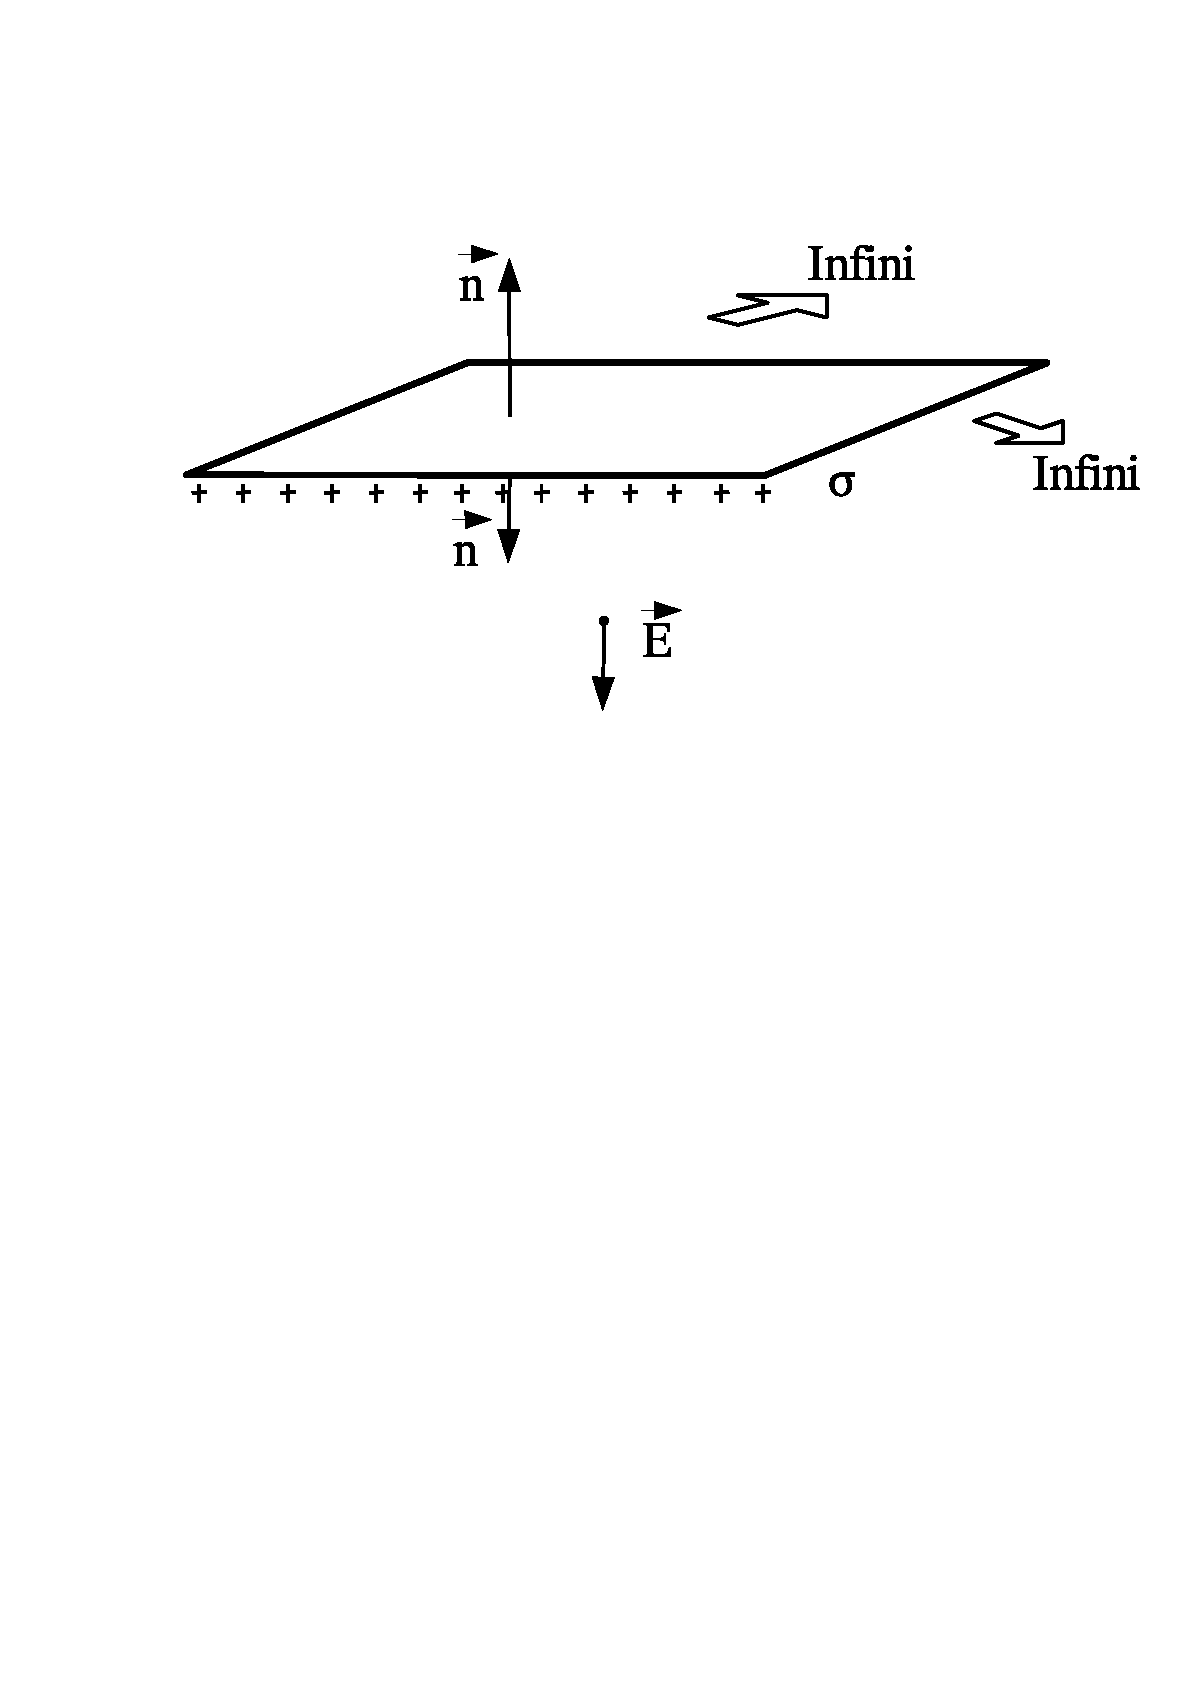
\includegraphics[clip=true,viewport=0cm 16.5cm 20cm 25cm,scale=0.38]{./figures/plaque_chargee.pdf}
\caption{Champ �lectrique g�n�r� par une plaque charg�e infinie.}\label{plaq_char_inf}
\end{center}
\end{figure}

Ce champ ne d�pend pas de la distance � la plaque et vaut~:
\begin{equation}\label{champ_cond_plan}
\vec {E} = \frac{\sigma }{2\varepsilon_{0}} \, \vec{n}
\end{equation}

Soient deux armatures $(A_{1})$ et $(A_{2})$ planes parall�les infinies, situ�es � une distance $d$ l'une de l'autre. L'armature $(A_{1})$ porte une densit� surfacique de charge $\sigma $ et $(A_{2})$ porte une densit� $-\sigma $. Selon le principe de superposition vu � la section \ref{princ_superpo}, le champ �lectrostatique entre les deux armatures est �gal � la superposition des champs cr��s par ces deux plans infinis (voir figure \ref{2_plaq}).

\begin{figure}[h]
\begin{center}
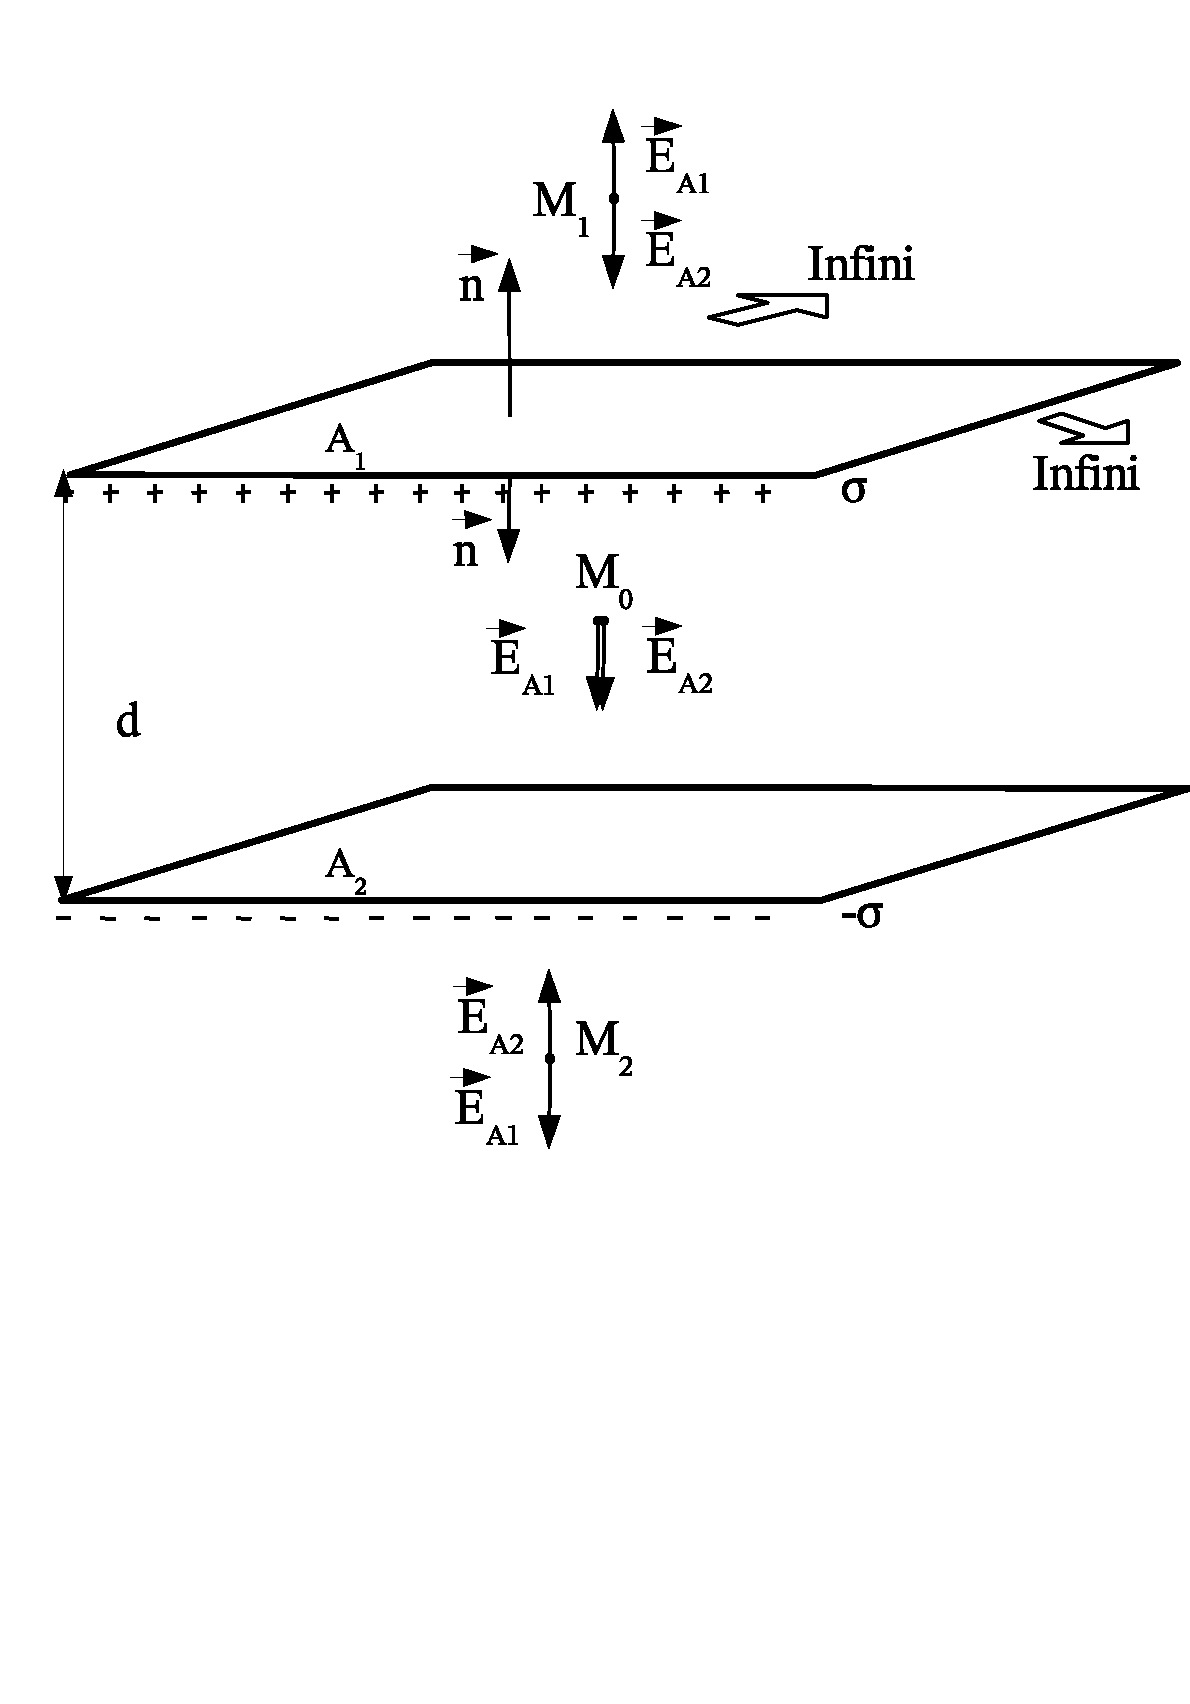
\includegraphics[clip=true,viewport=0cm 9cm 20cm 27cm,scale=0.33]{./figures/deux_plaques_chargees.pdf}
\caption{Champ �lectrique g�n�r� par deux plaques charg�es infinies.}\label{2_plaq}
\end{center}
\end{figure}

Ainsi,

\begin{equation}
\vec{E}(M_{1})=\vec{E}(M_{2})=0 \qquad \textrm{et} \qquad
\vec{E}(M_{0})=\vec{E_{A_{1}}} + \vec{E_{A_{2}}} = \frac{\sigma }{2\varepsilon_{0}}\vec{i} + \frac{-\sigma }{2\varepsilon_{0}} \, -\vec{i} = \frac{\sigma }{\varepsilon_{0}} \, \vec{i}.
\end{equation}

La capacit� $C$ d'un condensateur est le rapport de sa charge $Q$ et de la tension $U$ appliqu�e � ses bornes tel que :

\begin{equation}
 C=\frac{Q}{U}
\end{equation}

o� $U$ est donc la diff�rence de potentiel (ou circulation) entre les deux armatures telle que :

$$U = V_{1} - V_{2} = \int_{x_{1}}^{x_{2}} \vec{E}\cdot \vec{\ud x}=\frac{\sigma }{\varepsilon_{0}} \, d.$$

Puisque $Q=\sigma S$, $S$ �tant la surface de la plaque finie du condensateur, et $Q=CU$, on peut d�duire la capacit� $C$ du condensateur~:

\begin{equation}\label{capac_cond}
\boxed{C=\frac{\varepsilon_{0} \, S}{d}.}
\end{equation}

Pour obtenir une grande capacit�, il faut $S$ grand et/ou $d$ petit.

\begin{rem}[Effets de bords]
Les plaques d'un condensateur ne sont pas infinies, et le champ $\vec{E}$ n'est pas brusquement nul sur les bords. La valeur r�elle de $C$ est donc un peu plus �lev�e que la valeur th�orique. On corrige alors la surface $S$ telle que la plaque soit augment�e d'une longueur �gale � $\fractext{3}{8}d$.

\begin{figure}[h]
\begin{center}
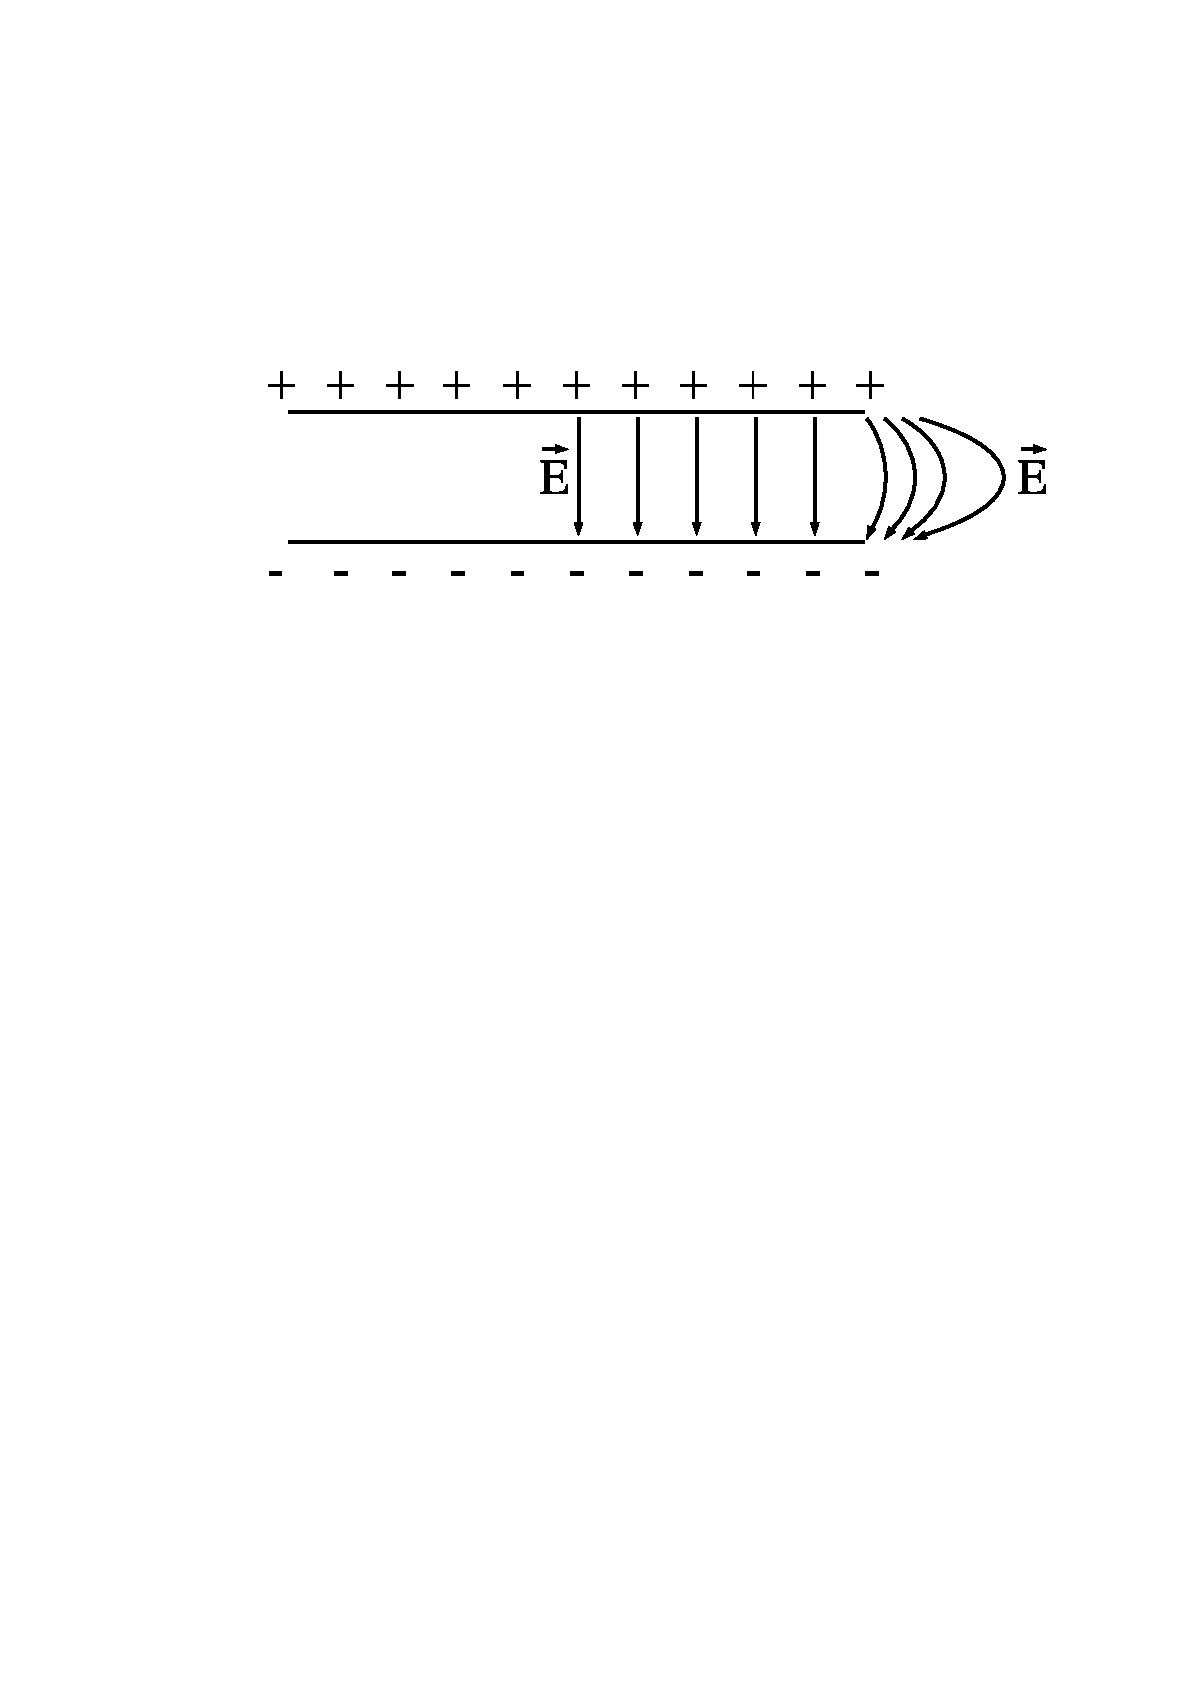
\includegraphics[clip=true,viewport=0cm 19cm 20cm 23cm,scale=0.38]{./figures/Effets_de_bords.pdf}
\caption{Effets de bords.}
\end{center}
\end{figure}
\end{rem}

\begin{rem}[Unit�]
L'unit� de la capacit� �lectrique est le Farad (Coulomb/Volt). Ceci donne une unit� pour la permittivit� en $\mathrm{Fm^{-1}}$. Les valeurs typiques de capacit� vont de $1\ \mathrm{pF}$ � quelques mF. Par exemple, si $S=1 \, \mathrm{cm^{2}}$ et $d=1\ \mathrm{mm}$, on a $C \approx 1 \mu \mathrm{F}$.
\end{rem}

\begin{bex}[Condensateur sph�rique]
A voir en TD
\end{bex}

\begin{bex}[Condensateur cylindrique]
A voir en TD
\end{bex}

\subsection{Condensateur en pr�sence d'un di�lectrique}

\paragraph{Exp�rience de Faraday.}La capacit� d'un condensateur augmente si on introduit un isolant entre ses plaques. Si l'isolant remplit tout l'espace inter-plaque, la capacit� est multipli�e par $\varepsilon_{r}$ qui ne d�pend que de la nature de l'isolant (ou di�lectrique).

Dans les isolants, les �lectrons des couches externes forment des \textbf{liaisons covalentes}, \textbf{ioniques} ou plus g�n�ralement \textbf{ionocovalentes}. Dans ce type de liaison, un �lectron ne s'�loigne jamais de l'atome dont il est issu, tout au plus s'en �carte-t-il pour atteindre les premiers atomes voisins. Chaque �lectron reste localis� dans une r�gion tr�s restreinte de l'espace. Il n'est donc pas mobile.

\begin{figure}[h]
\begin{center}
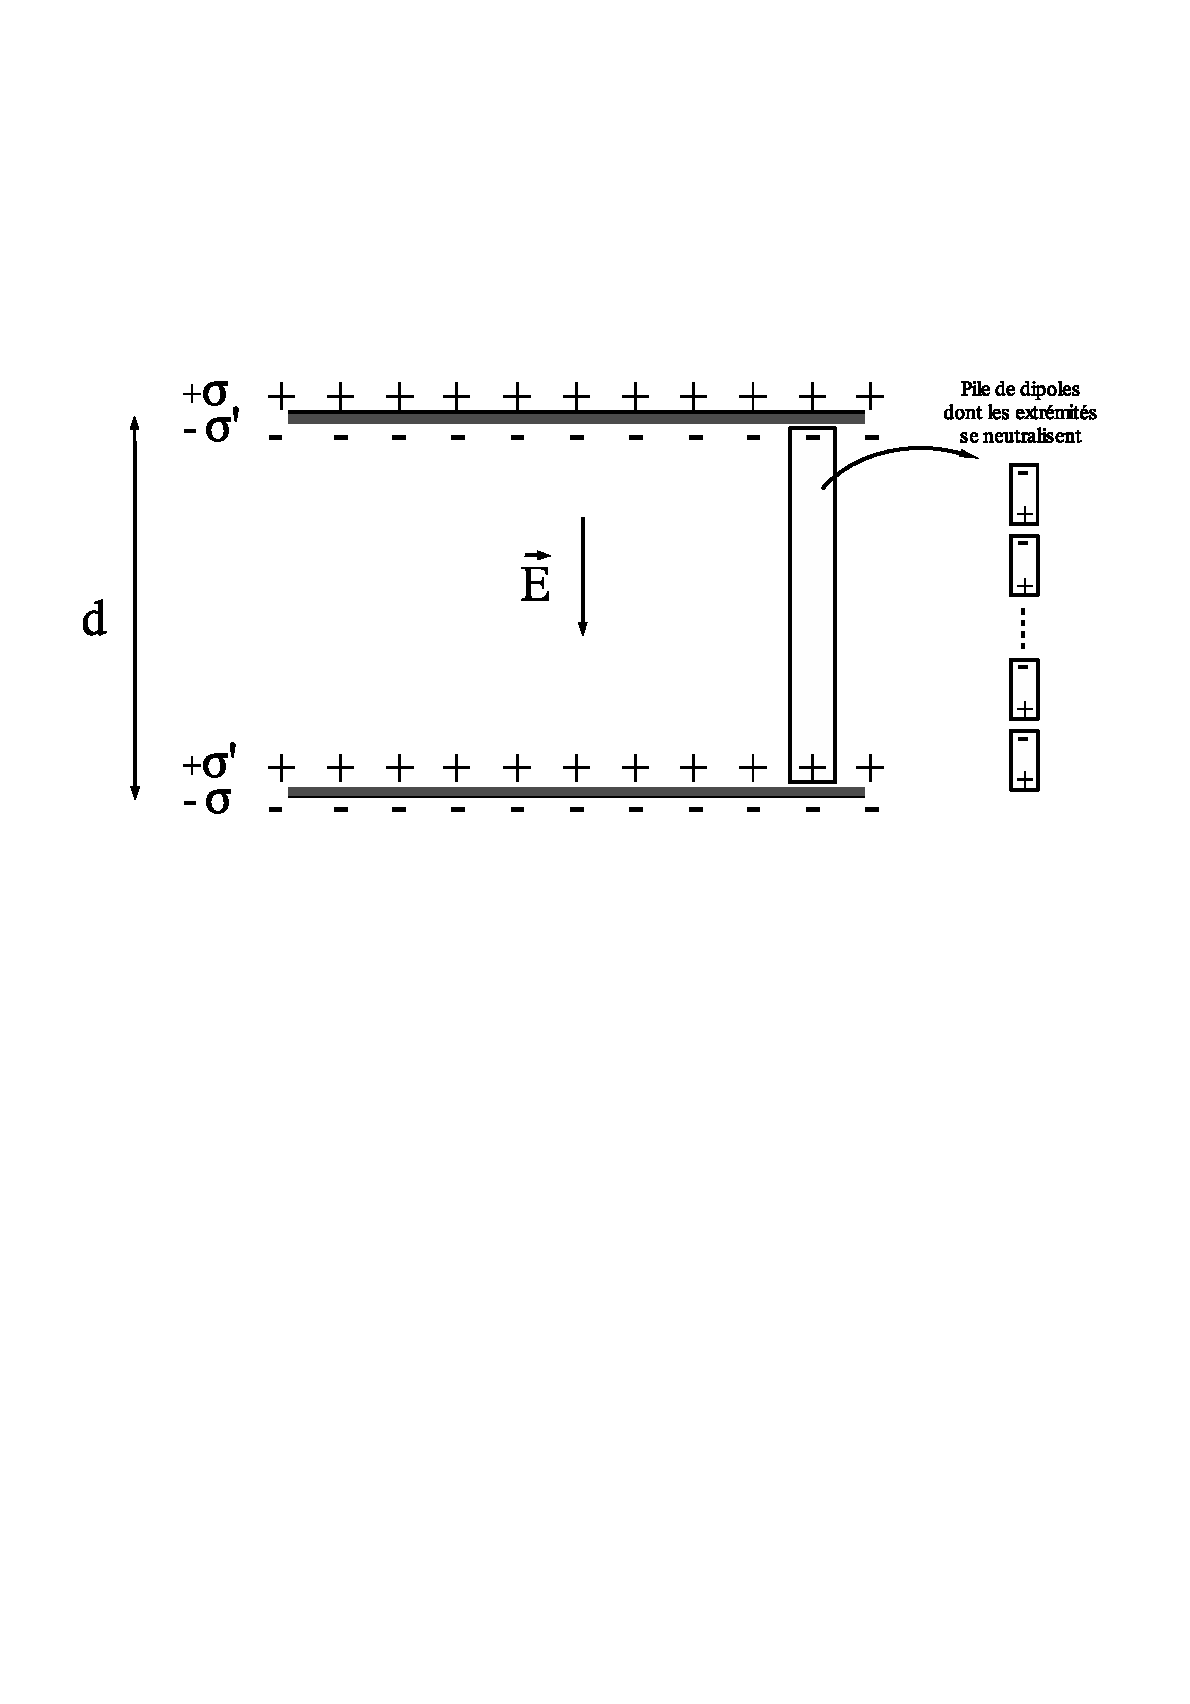
\includegraphics[clip=true,viewport=0cm 15cm 20cm 23cm,scale=0.38]{./figures/polarisation_dielectrique.pdf}
\caption{Polarisation du di�lectrique.}
\end{center}
\end{figure}


La \textbf{polarisation du di�lectrique} s'�crit~:
\begin{equation}\label{pola_dielec}
 \vec{P}=\varepsilon_{0} \chi \vec{E}
\end{equation}polarisation du di�lectrique
\noindent o� $\chi$ est la \textbf{suceptibilit� di�lectrique}. D'autre part on a:
\begin{equation}
 \vec{E}= \frac{\sigma - P}{\varepsilon_{0}} \, \vec{dir}_{E}.
\end{equation}
Cette derni�re �quation conduit � un champ �lectrique diminu� tel que:
\begin{equation}
 E=\frac{\sigma }{(1+\chi)\varepsilon_{0}}.
\end{equation}

On appelle respectivement \textbf{permittivit� absolue} et \textbf{permittivit� relative} du di�lectrique les grandeurs (cf. tableau \ref{tab_epsilonR}):
$$\varepsilon =\varepsilon_{r} \varepsilon_{0}
\qquad \textrm{et} \qquad
\varepsilon_{r} =1+\chi.$$

La diff�rence de potentiel entre ses bornes s'�crit donc~:
\begin{equation*}
\begin{split}
U = V_{1} - V_{2} & = \int_{x_{1}}^{x_{2}} \vec{E}\cdot \vec{\ud x} \\
& = Ed \\
& = \frac{\sigma \,d}{\varepsilon_{r}\varepsilon_{0}} \\
& = \frac{Q}{C^{\prime} }
\end{split}
\end{equation*}

\noindent o� l'on a pos� $C^{\prime} = \fractext{\varepsilon_{r}\varepsilon_{0}\ S}{d}$.

\begin{rem}[Ordre de grandeur]
\mbox{}
$\varepsilon_{r}=1$ dans le vide ;
$\varepsilon_{r}=1.0001$ dans l'air ;
$\varepsilon_{r}=4$ � $7$ du verre ;
$\varepsilon_{r}=80$ dans l'eau pure ;
$\varepsilon_{r}=1000$ dans certains cristaux. Au del� d'un certain potentiel, les di�lectriques peuvent conduire le courant (tension de claquage marqu� sur les condensateurs). Le di�lectrique est alors en parti d�truit. (Voir aussi tableau \ref{tab_epsilonR}).
\end{rem}


\subsection{Association des condensateurs}

\subsubsection{En parall�le}

Le potentiel est identique aux bornes de chaque condensateur. Les charges s'additionnent donc et on obtient:

$$Q_{1}=UC_{1} \quad Q_{2}=UC_{2} \quad \cdots \quad Q_{n}=UC_{n}$$
$$Q_{E}=\sum_{i=1}^{n}Q_{i}=U \sum_{i=1}^{n}C_{i}$$
\begin{equation}\label{cond_parall}
 \boxed{C_{E}=\sum_{i=1}^{n}C_{i}}
\end{equation}

\begin{figure}[ht]
\begin{center}
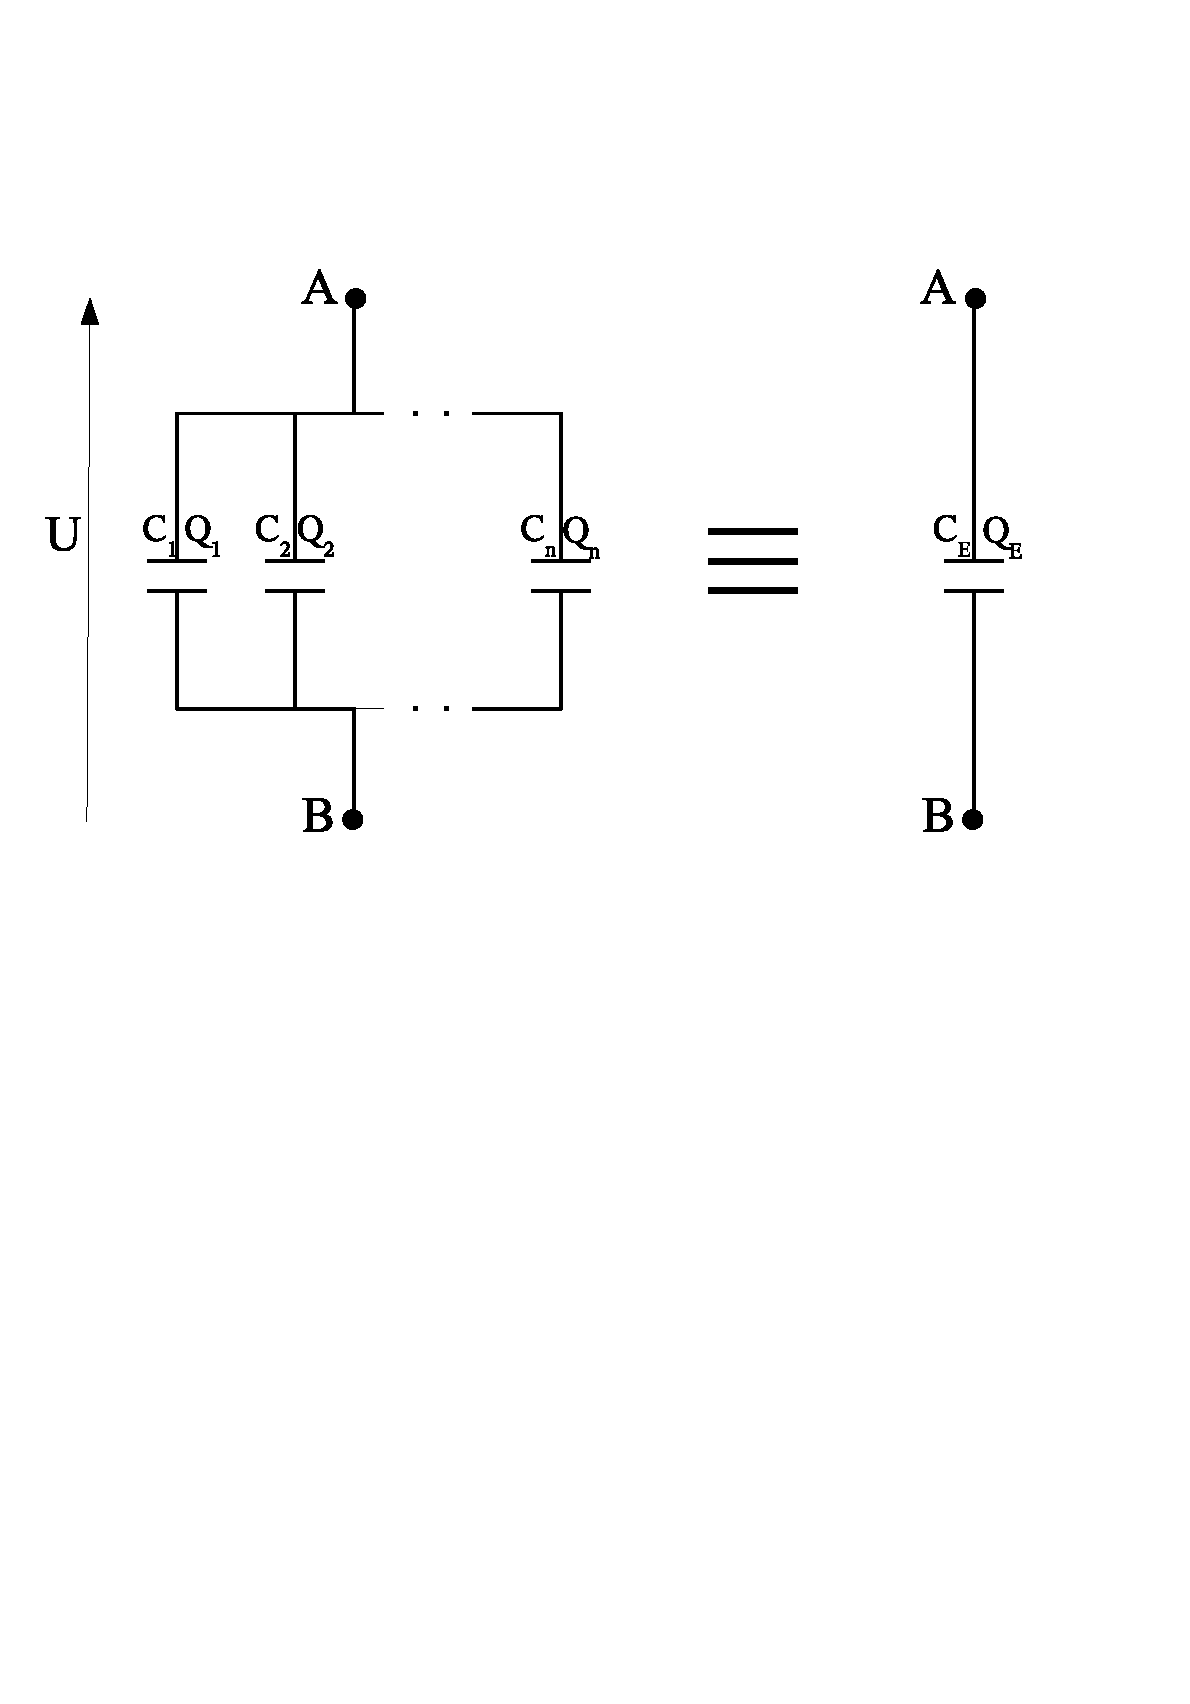
\includegraphics[clip=true,viewport=0cm 14cm 20cm 24.5cm,scale=0.38]{./figures/association_C_parallele.pdf}
\caption{Association de condensateurs en parall�le.}
\end{center}
\end{figure}

\subsubsection{En s�rie}

La charge est identique dans chaque condensateur. Les tensions s'additionnent, d'o�~:

$$U_{1}=\frac{Q}{C_{1}} \quad U_{2}=\frac{Q}{C_{2}} \quad \cdots \quad U_{n}=\frac{Q}{C_{n}}$$
$$U_{E}=\sum_{i=1}^{n}U_{i}=Q \sum_{i=1}^{n} \frac{1}{C_{i}}$$
\begin{equation}\label{cond_serie}
 \boxed{\frac{1}{C_{E}}=\sum_{i=1}^{n} \frac{1}{C_{i}}}
\end{equation}

\begin{figure}[ht]
\begin{center}
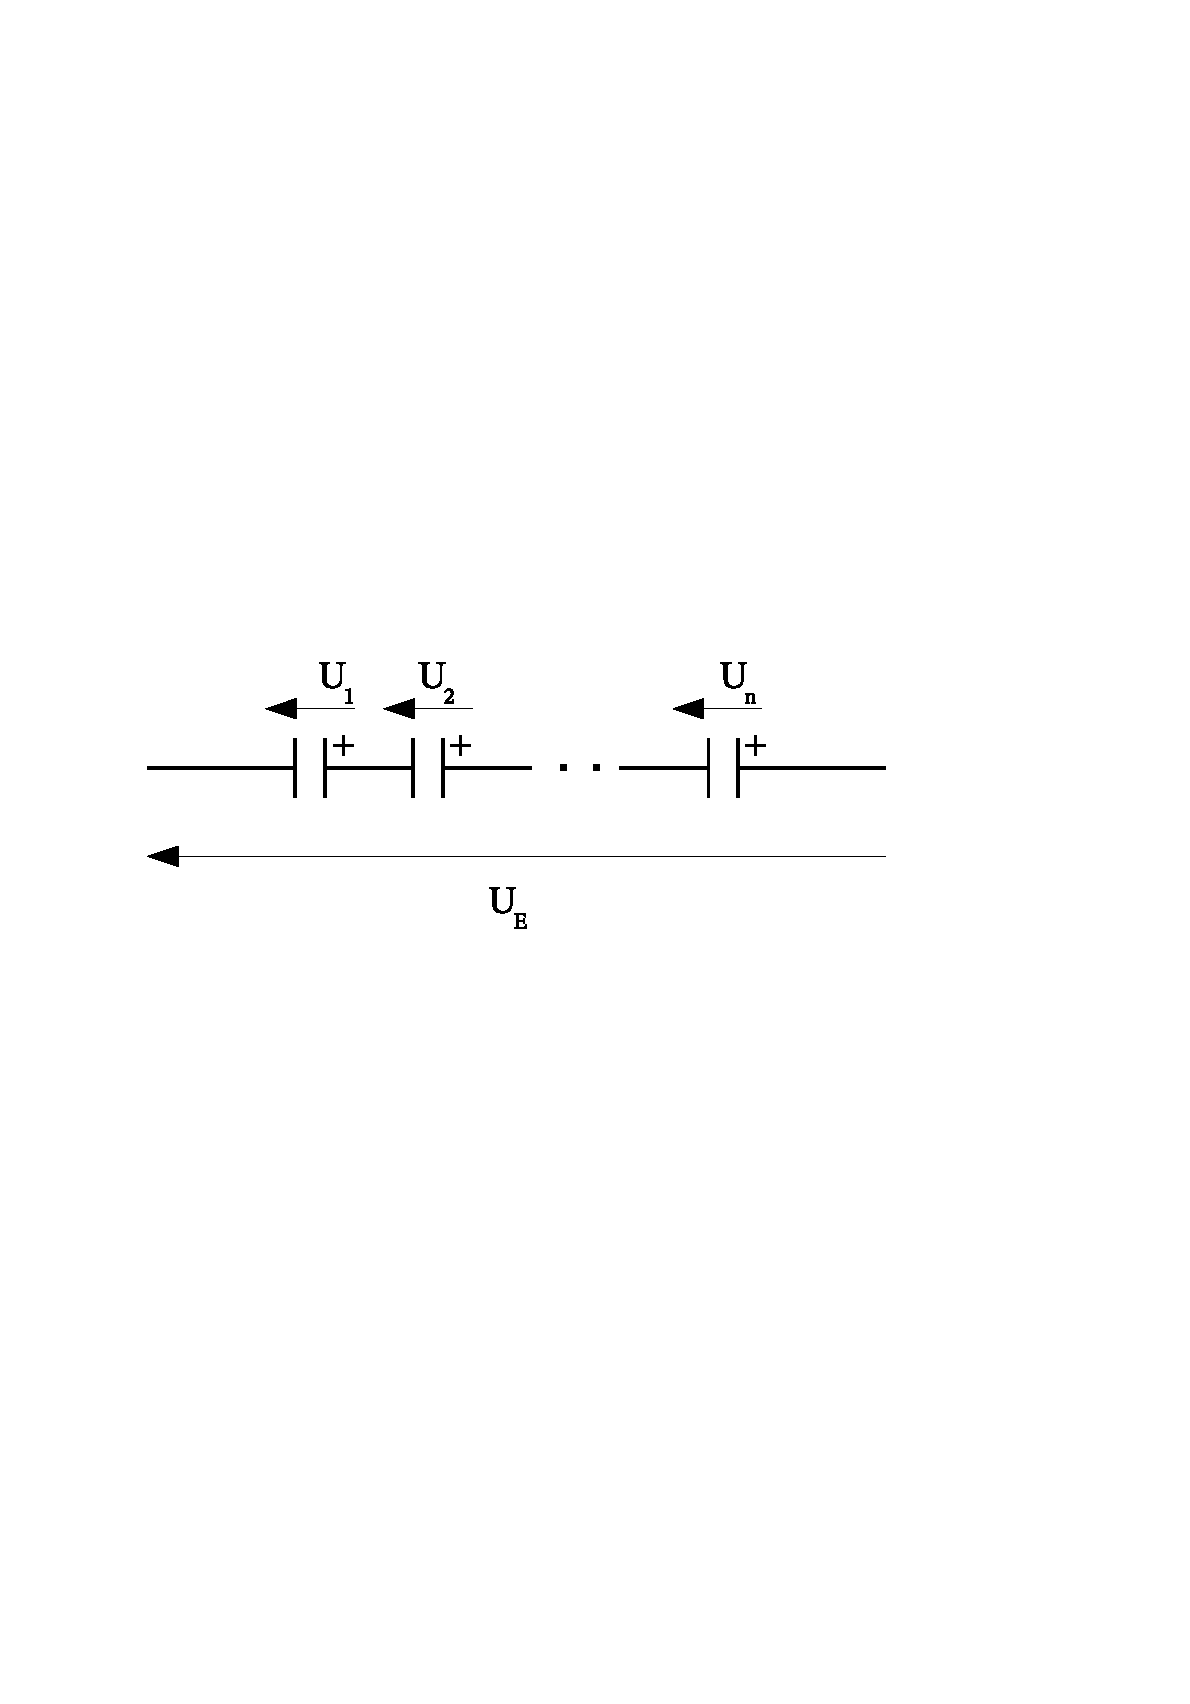
\includegraphics[clip=true,viewport=0cm 13cm 20cm 19cm,scale=0.38]{./figures/association_C_serie.pdf}
\caption{Association de condensateurs en s�rie.}
\end{center}
\end{figure}

%\subsection{Energie emmagasin�e par un condensateur}

\subsection{Notions sur les �lectrets}

Un \textbf{�lectret} est un mat�riau suceptible de conserver en permanence une polarisation �lectrique, m�me en absence de champ �lectrique.

Exemple de mat�riaux : T�flon, Mylar (TM).

Exemple d'utilisation : microphones � condensateur sans avoir besoin de tension continue de polarisation (miniaturisation).

Mode de fabrication : bombardement d'�lectrons ou d'ions pour soumettre le di�lectrique � l'action d'un champ �lectrique intense. Ces mat�riaux g�n�rent un champ �lectrique constant m�me apr�s l'arr�t du bombardement (analogie avec les aimants).


\cleardoublepage

\chapter{Electrocin�tique}\label{chap_eleccine}

\section{Rappels}
\subsection{Mobilit� des charges~: courant �lectrique}

Soit deux conducteurs $A$ et $B$ isol�s en �quilibre avec $V_{A} > V_{B}$ (voir figure \ref{cond_charge}). $A$ poss�de en exc�s des charges positives et $B$ poss�de en exc�s des charges n�gatives.

\begin{figure}[h]
\begin{center}
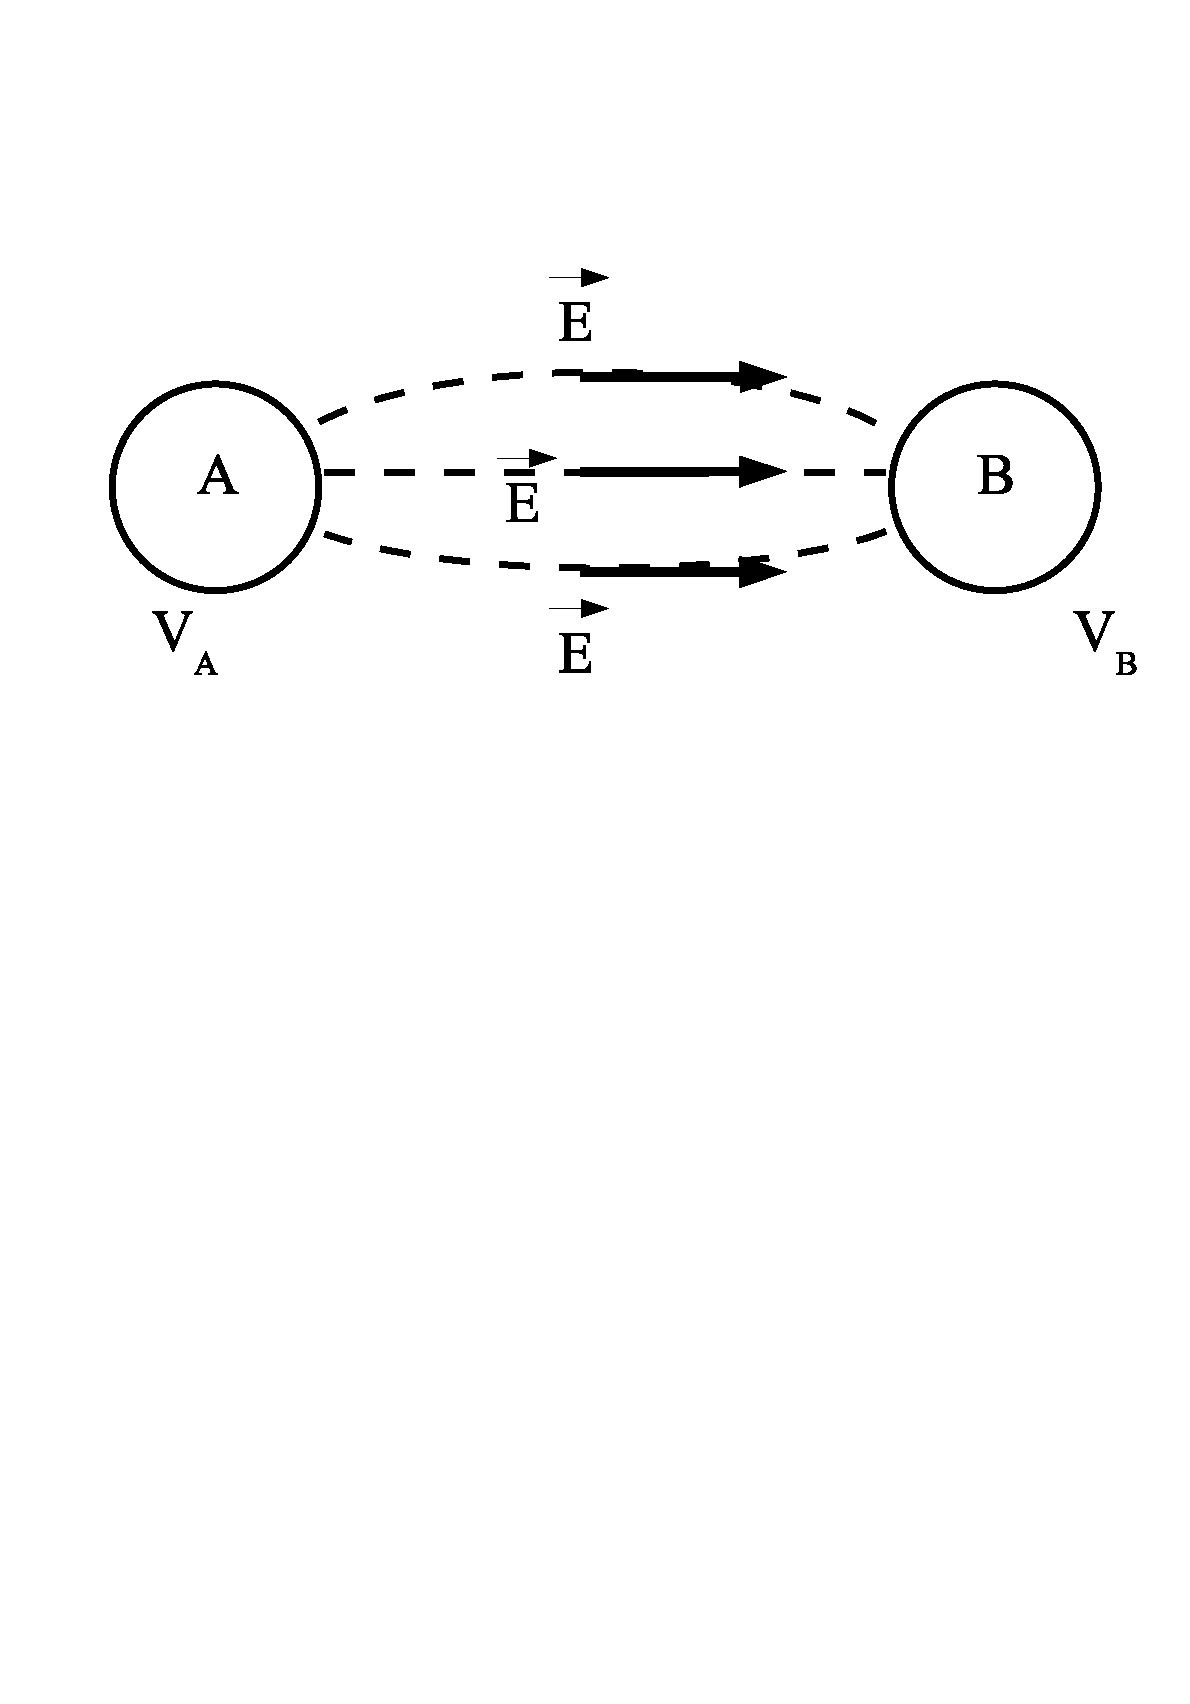
\includegraphics[clip=true,viewport=0cm 17cm 20cm 25cm,scale=0.38]{./figures/Conducteurs_charges.pdf}
\caption{Conducteurs charg�s isol�s en �quilibre.}\label{cond_charge}
\end{center}
\end{figure}

Si on relie les deux conducteurs par un fil �galement conducteur, il y a un transfert de charge pour que tout point soit au m�me potentiel. Ensuite, $A$ et $B$ sont au m�me potentiel, le champ �lectrique s'annule alors ainsi que le courant.

Le d�placement des �lectrons libres est quasiment instantan� (r�gime transitoire). Supposons que le pr�c�dent conducteur isol� $B$ soit un r�servoir d'�lectrons libres, c'est-�-dire que l'on arrive � maintenir son potentiel $V_{B}$. Si on fait en sorte que les �lectrons exc�dentaires du conducteur $A$ quittent le mat�riau pour maintenir le potentiel $V_{A}$, le champ �lectrique initial est r�tabli et le d�placement des �lectrons � l'int�rieur du fil conducteur est entretenu. Le champ $\vec{E}$ qui assure le d�placement des �lectrons et la circulation du courant est appel� \textbf{champ �lectromoteur}.

\subsection {Densit� de courant �lectrique}

\begin{figure}[h]
\begin{center}
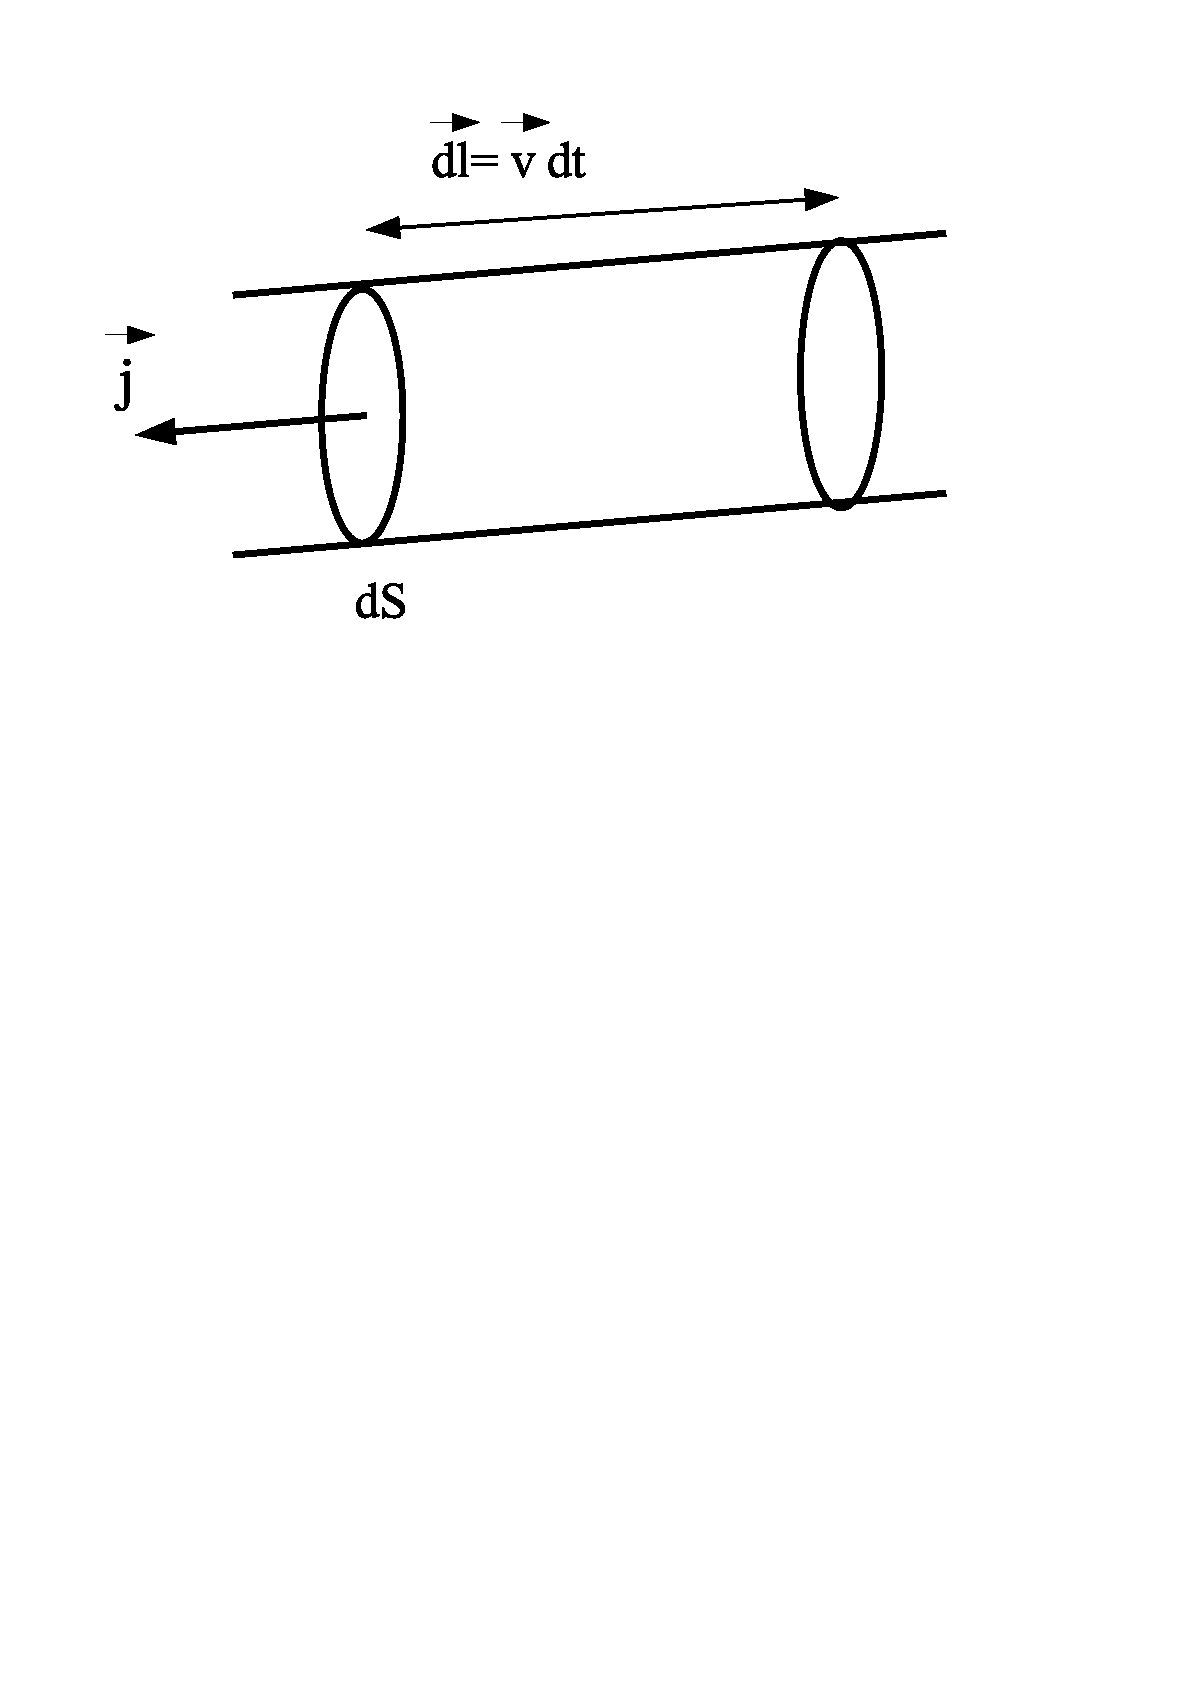
\includegraphics[clip=true,viewport=0cm 18cm 20cm 27cm,scale=0.38]{./figures/densite_de_courant.pdf}
\caption{Param�trisation d'un �l�ment de fil pour le calcul du courant.}\label{sch_cour}
\end{center}
\end{figure}

Le courant est produit par un d�placement organis� de charges, � une certaine vitesse. Consid�rons un fil conducteur de section $S$, dans lequel se trouve une densit� de charge volumique $\rho$, anim� d'une vitesse $\vec{v}$ (cf. figure \ref{sch_cour}). Pendant un instant $\ud t$, ces charges parcourent une distance $\vec{v} \ud t$. Soit $\vec{n} \ud S$ un �l�ment infinit�simal de surface mesur�e sur la section du fil, orient� dans une direction arbitraire. La quantit� de charge �lectrique qui traverse cette surface pendant $\ud t$ est celle contenue dans le volume �l�mentaire $\ud V$ associ� et s'�crit~:

$$\ud Q = \rho \ud V = \rho \vec{v} \ud t \cdot \vec{n} \ud S$$

On voit alors appara�tre un vecteur qui d�crit les caract�ristiques du milieu conducteur et qu'on appelle la \textbf{densit� de courant}~:

$$\vec{j} = \rho \vec{v}$$

exprim� en Amp�res par m�tre carr� ($\mathrm{A.m^{-2}}$).

Le courant $dI$ circulant dans la portion de fil est la charge traversant la section, et est reli� � la densit� tel que~:

$$\ud I = \frac{\ud Q}{\ud t}$$

On en d�duit :

$$I = \frac{1}{\ud t} \iint_{S} \ud Q = \frac{1}{\ud t} \iint_{S} \vec{j} \ud t \cdot \vec{n} \ud S$$

soit :

\begin{equation}
\boxed{I = \iint_{S} \vec{j} \cdot \vec{n} \ud S}
\end{equation}

On avait d�finit le flux du champ �lectrique~: $\Phi = \iint_{S} \vec{E} \cdot \vec{n} \ud S$. De m�me, $I$ est le flux de la densit� de courant � travers la section du fil. Le sens du courant est donn� par le sens du vecteur densit� de courant.

\begin{rem}[Convention]
On suppose que le courant est d� au mouvement des charges positives vers les charges n�gatives : sens du courant. En fait, ce sont les �lectrons libres qui se d�placent, mais on conserve la convention pour des raisons historiques.
\end{rem}


\subsection{Loi d'Ohm locale (ou microscopique)}

Dans la plupart des conducteurs, on observe une proportionnalit� entre le densit� de courant et le champ �lectrostatique local~:

\begin{equation}
\boxed{\vec{j}=\gamma \vec{E}},
\end{equation}

o� le c\oe fficient de proportionnalit� $\gamma $ est appel� la \textbf{conductivit� du milieu}. La conductivit� est une grandeur locale positive d�pendant uniquement des propri�t�s du mat�riau, elle s'exprime en Siemens par m�tre et est �gale � l'inverse de la r�sistivit� du milieu $\eta = 1/\gamma $. Par exemple, le cuivre poss�de une conductivit� $\gamma_{Cu} = 58.10^{6}\  \mathrm{S.m^{-1}}$, tandis que celle du verre (isolant) est $\gamma_{Cu} = 10^{-11}\ \mathrm{S.m^{-1}}$.

\subsection{R�sistance d'un conducteur. Loi d'Ohm}

Consid�rons maintenant une portion AB d'un conducteur parcouru par un courant $I$. S'il existe un courant $I = \iint_{S} \vec{j} \cdot \vec{n} \ud S$, cela signifie qu'il y a une chute de potentiel entre $A$ et $B$, $U=V_{A} - V_ {B}=\int_{A}^{B} \vec{E} \cdot \vec{\ud l}$. Il existe un scalaire $R$, caract�ristique du conducteur, tel que~:

\begin{equation}\label{resist_cond}
R = \frac{U}{I} = \frac {\int_{A}^{B} \vec{E} \cdot \vec{\ud l}}{\iint_{S} \vec{j} \cdot \vec{n} \ud S} =\frac {\int_{A}^{B} \vec{E} \cdot \vec{\ud l}}{\iint_{S} \gamma  \vec{E} \cdot \vec{n} \ud S},
\end{equation}

o� l'unit� est l'Ohm (symbole $\Omega$).

\begin{bex}[Fil cylindrique homog�ne]
Dans le cas simple d'un conducteur filiforme de section $S$ o�, sur une longueur $L$, le champ �lectrostatique est uniforme, on obtient le lien entre la r�sistance d'un conducteur (propri�t� macroscopique) et sa r�sistivit� (propri�t� microscopique) tel que :

\begin{equation}\label{resist_fil}
R = \frac{E L}{\gamma E S}=\eta \frac{L}{S}
\end{equation}

dont l'unit� est le $\Omega.m$ (Ohm m�tre).
\end{bex}


\subsection{Association de r�sistances}

\subsubsection{R�sistances en s�rie}

Soient $n$ r�sistances $R_{i}$ mises bout � bout dans un circuit et parcourues par un courant $I$. La tension aux bornes de la cha�ne s'�crit simplement~:

$$U = (V_{0} - V_{1}) + (V_{1} - V_{2}) + \cdots + (V_{n-1} - V_{n})=R_{1} I + R_{2} I+ \cdots + R_{n} I,$$

Le r�sistance totale est donc analogue � celle obtenue par une r�sistance unique dont la valeur est~:

\begin{equation}
\boxed{R = \sum_{i=1}^{n}R_{i}.}
\end{equation}

\subsubsection{R�sistances en parall�le}

Soient $n$ r�sistances $R_{i}$ branch�es en parall�le sous une tension $U = V_{1} - V_{2}$ et aliment�es par un courant $I$. Le courant se s�pare alors en $n$ courants~:

$$I_{i} = \frac{U}{R_{i}},$$

dans chacune des $n$ branches. Nous avons alors (propri�t� de conservation du courant)~:

$$I = \sum_{i=1}^{n} I_{i} = \sum_{i=1}^{n} \frac{U}{R_{i}} = \frac{U}{R},$$

c'est-�-dire que l'ensemble des $n$ branches est analogue � une r�sistance �quivalente en s�rie �gale � :

\begin{equation}
\boxed{\frac{1}{R} = \sum_{i=1}^{n} \frac{1}{R_{i}}}
\end{equation}


\section{El�ments d'un circuit �lectrique}

\subsection{Notion de circuit �lectrique}

\begin{defi} Un circuit �lectrique est constitu� d'un ensemble de dispositifs appel�s \textbf{dip�les}, reli�s entre eux par un fil conducteur et formant ainsi une structure ferm�e. Un \textbf{n\oe ud} d'un circuit est une interconnexion o� arrivent 3 fils ou plus. Une \textbf{branche} est un tron�on de circuit situ� entre deux n\oe uds. Enfin, une \textbf{maille} est un ensemble de branches formant une boucle ferm�e.
\end{defi}

Un \textbf{dip�le} s'ins�re dans un circuit par l'interm�diaire de deux p�les, l'un par o� s'effectue l'entr�e du courant (borne $+$), l'autre la sortie (borne $-$). Il est caract�ris� par sa r�ponse � une diff�rence de potentiel $U$ entre ses bornes~: c'est-�-dire la courbe caract�ristique $I=f(U)$ qui, pour un dip�le passif, passe par l'origine. Un dip�le actif fournit un courant (positif ou n�gatif) m�me en absence de tension. Enfin, on appelle dip�le lin�aire tout dip�le dont la courbe est une droite.

Nous avons vu que, dans tout conducteur, la pr�sence d'une r�sistivit� entra�ne une variation de tension entre 2 noeuds travers�s par le m�me courant. Les fils �lectriques reliant les dip�les imposent ainsi leurs r�sistances propres qui s'ajoutent � la r�sistance globale du circuit. Dans la majorit� des cas d'�lectronique de puissance, ces r�sistances internes sont faibles devant celles des dip�les. Les fils sont alors suppos�s �quipotentiels. Cette hypoth�se n'est par contre plus valable dans le cas de courants de faible intensit� (�lectronique fine, micro-processeurs, etc...).

\begin{rem}
Nous nous int�ressons ici � des cas o� le courant est �tabli de fa�on permanente dans le circuit. L'intensit� y est alors la m�me en tout point. Cela exige �videmment que le circuit soit \emph{ferm�}.
\end{rem}

\subsection{Puissance �lectrique disponible}

Soit une portion $AB$ d'un circuit, parcourue par un courant permanent $I$ allant de $A$ vers $B$. L'existence de ce courant implique que le potentiel en $A$ est sup�rieur � celui en $B$. Cette diff�rence de potentiel se traduit par l'existence d'un champ �lectrostatique $\vec{E}$ produisant une force de Coulomb $\vec{F} = q \vec{E}$ capable d'acc�l�rer une charge $q$. Ainsi, soit $P_{q} = \vec{v} \cdot \vec{E}$ la puissance n�cessaire pour communiquer une vitesse $\vec{v}$ � une particule de charge $q$ quelconque. Sachant que dans ce conducteur il y a $n$ porteurs de charge par unit� de volume, la puissance totale $P$ mise en jeu dans le brin $AB$ parcouru par un courant $I$ s'�crit~:

\begin{equation*}
\begin{split}
P & = \iiint_{brin AB} nP_{q}\ \ud V \\
& = \int_{A}^{B} \iint_{Section} (nq\vec{v} \cdot \vec{dS}) \vec{E} \cdot \vec{\ud l} \\
& = \int_{A}^{B} \vec{E} \cdot \vec{\ud l} \iint_{Section} \vec{j} \cdot \vec{\ud S} \\
& = I \int_{A}^{B} \vec{E} \cdot \vec{\ud l} = I [V(A) - V(B)].
\end{split}
\end{equation*}

On en d�duit:

\begin{equation}
\boxed{P = UI}
\end{equation}

o� $U = V(A) - V(B) >0$ puisque le courant s'�coule de $A$ vers $B$. Cette puissance est donc la puissance �lectrique disponible entre $A$ et $B$ du simple fait qu'il y circule un courant $I$.

Suivant la nature du dip�le plac� entre $A$ et $B$ (r�cepteur), l'�nergie �lectrique disponible sera convertie sous une forme ou une autre. Dans le cas simple o� entre $A$ et $B$ ne se trouve qu'une r�sistance $R$, la puissance disponible $P$ ne sert qu'� faire chauffer la r�sistance puisque $U = RI$. Cela se traduit par une dissipation d'�nergie sous forme de chaleur, appel�e effet Joule, et dont la puissance vaut~:

\begin{equation}\label{joule}
\boxed{P_{j}=RI^{2}.}
\end{equation}

Cette �nergie peut �tre �galement reconvertie en rayonnement (lampe), �nergie m�canique (moteur), chimique (bac � �lectrolyse).

\begin{rem} Cette puissance peut aussi �tre n�gative lorsque $U = V(A) - V(B) <0$. Le dip�le fournit alors de l'�nergie, c'est un g�n�rateur.
\end{rem}

\subsection{N�cessit� d'une force �lectromotrice ou f�m}

Si on applique le raisonnement pr�c�dent � un circuit ferm�, c'est-�-dire si l'on regarde la puissance totale fournie entre $A$ et $B$ par la force de Coulomb, on obtient~:

$$P=I[V(A)-V(A)]=0,$$

c'est-�-dire une puissance nulle. Cela signifie qu'il ne peut y avoir de courant en r�gime permanent. Lorsqu'il y a un courant, cela implique que la force de Coulomb n'est pas responsable du mouvement global des porteurs de charge dans un conducteur.

\begin{rem}[Analogie]
Le courant dans un conducteur peut �tre compris avec l'analogie de la rivi�re circulant dans son lit. Pour qu'il y ait un �coulement, il faut que l'eau s'�coule d'une r�gion plus �lev�e vers une r�gion plus basse. Ainsi, le mouvement de l'eau d'un point �lev� vers un point plus bas est bien d� � la simple force de gravitation. Mais si l'on veut constituer un circuit ferm�, alors il faut fournir de l'�nergie (gr�ce � une pompe) pour amener l'eau � une plus grande hauteur, et le cycle peut alors effectivement recommencer.
\end{rem}

C'est exactement ce qui se passe dans un circuit �lectrique : une force autre que la force �lectrostatique doit permettre aux porteurs de charge de remonterle potentiel.

\begin{figure}[h]
\begin{center}
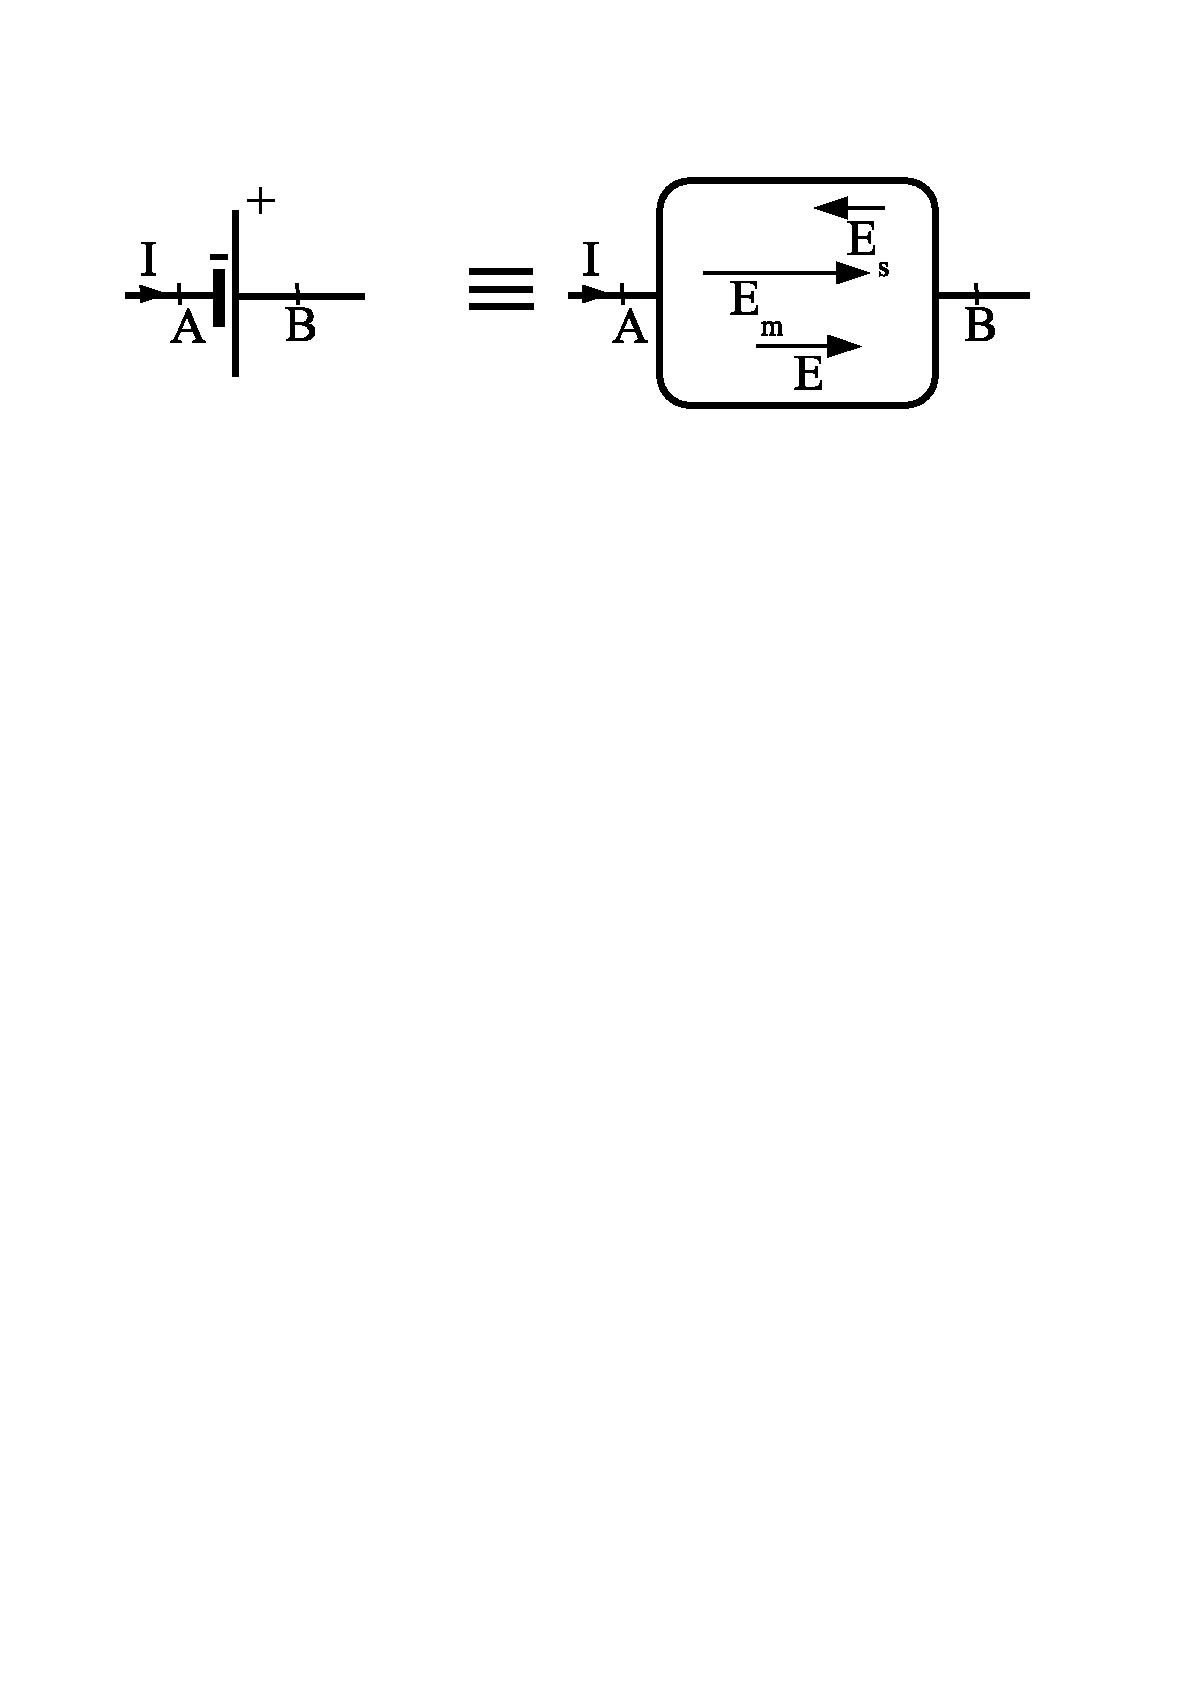
\includegraphics[clip=true,viewport=0cm 22cm 19cm 27cm,scale=0.55]{./figures/generateur.pdf}
\caption{Force responsable du courant.}
\end{center}
\end{figure}

La seule fa�on d'obtenir un r�gime stationnaire avec un courant permanent $I$, c'est donc d'avoir un champ suppl�mentaire, appel� champ �lectromoteur $\vec{E_{m}}$, sup�rieur en norme et dirig� en sens inverse de $\vec{E_{s}}$ (le champ �lectrostatique). Mettons maintenant le g�n�rateur en circuit ouvert ($I=0$). Le fait qu'une diff�rence de potentiel (ddp) se maintienne entre ses bornes implique n�cessairement la pr�sence d'une autre force compensant l'attraction coulombienne. Ainsi, � l'�quilibre et en l'absence de courant, on doit donc avoir $\vec{E_{s}} + \vec{E_{m}}=0$. Cela signifie donc que la ddp ou tension aux bornes d'un g�n�rateur ouvert vaut~:

$$V_{A}-V_{B}=\int_{A}^{B} \vec{E_{s}} \cdot \vec{\ud l}=-\int_{A}^{B} \vec{E_{m}} \cdot \vec{\ud l},$$

o�, bien �videmment, $V_{A}-V_{B}<0$. On appelle~:

$$e=\int_{A}^{B} \vec{E_{m}} \cdot \vec{\ud l}$$

\textbf{la force �lectromotrice} ou \textbf{f�m} du g�n�rateur ($e>0$ est exprim� en volts).

\subsection{Conventions}

Dans une branche, le sens du courant peut �tre choisi arbitrairement. L'orientation de la tension est ind�pendante du choix de l'orientation de l'intensit�~: $U_{AB}=V_A -V_B$ (de B vers A).\\

\begin{itemize}
\item Convention g�n�rateur~: $U$ et $I$ sont dans le m�me sens.
\item Convention r�cepteur~: $U$ et $I$ sont de sens contraire.\\
\end{itemize}

Si une branche contient un dip�le polaris� de f�m $e$, celui-ci sera compt� $+e$ si en parcourant la branche, on entre par la borne $-$ (au sens d'une chute de potentiel).

Exemple~:

\begin{figure}[h]
\begin{center}
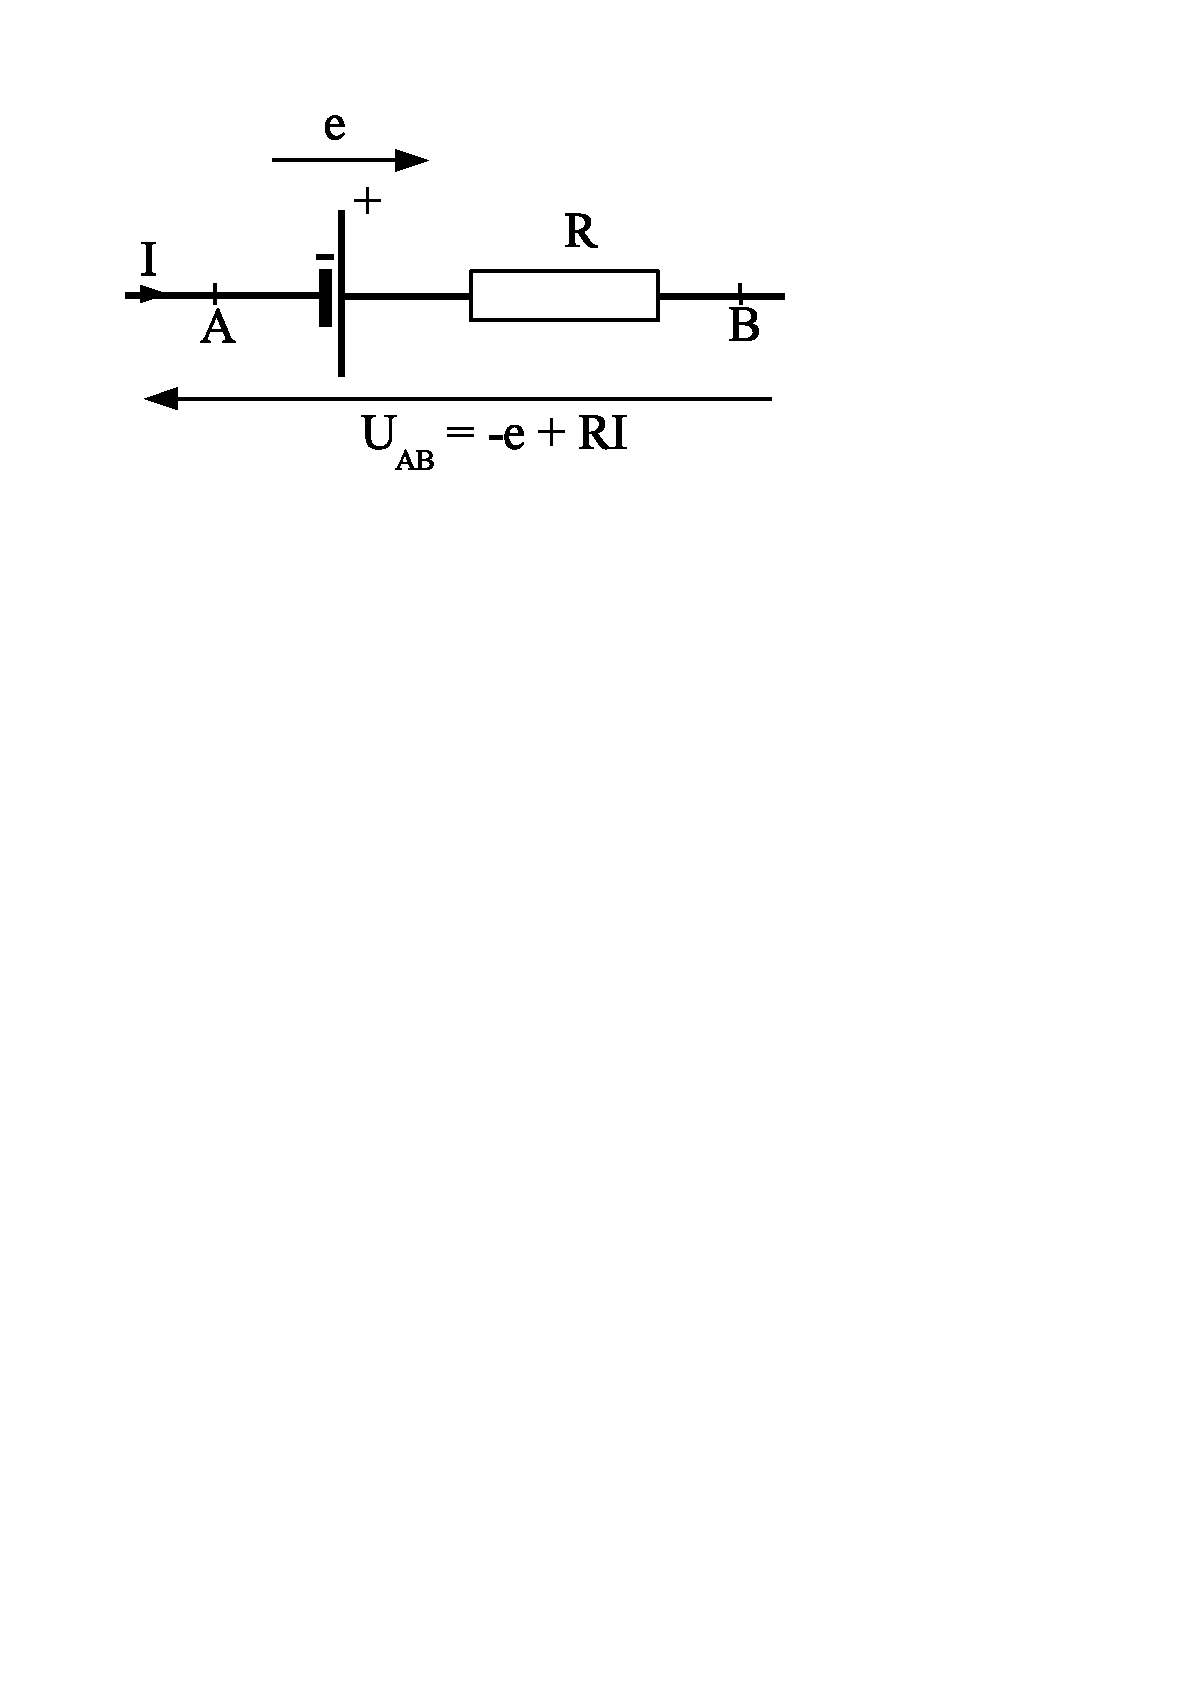
\includegraphics[clip=true,viewport=0cm 20.5cm 15cm 27cm,scale=0.65]{./figures/Calcul_de_tension.pdf}
\caption{Calcul de tension (exemple).}
\end{center}
\end{figure}

\subsection{Relation courant / tension}

Les dip�les sont caract�ris�s par une relation $U=f(I)$ ou $I=f(U)$ reliant la tension $U$ � leurs bornes au courant $I$ les traversant. Cette relation d�pend des dip�les. La repr�sentation graphique de cette relation s'appelle caract�ristique. Si cette caract�ristique passe par l'origine, le dip�le est dit passif ; dans le cas contraire, il est dit actif.

\begin{figure}[h]
\begin{center}
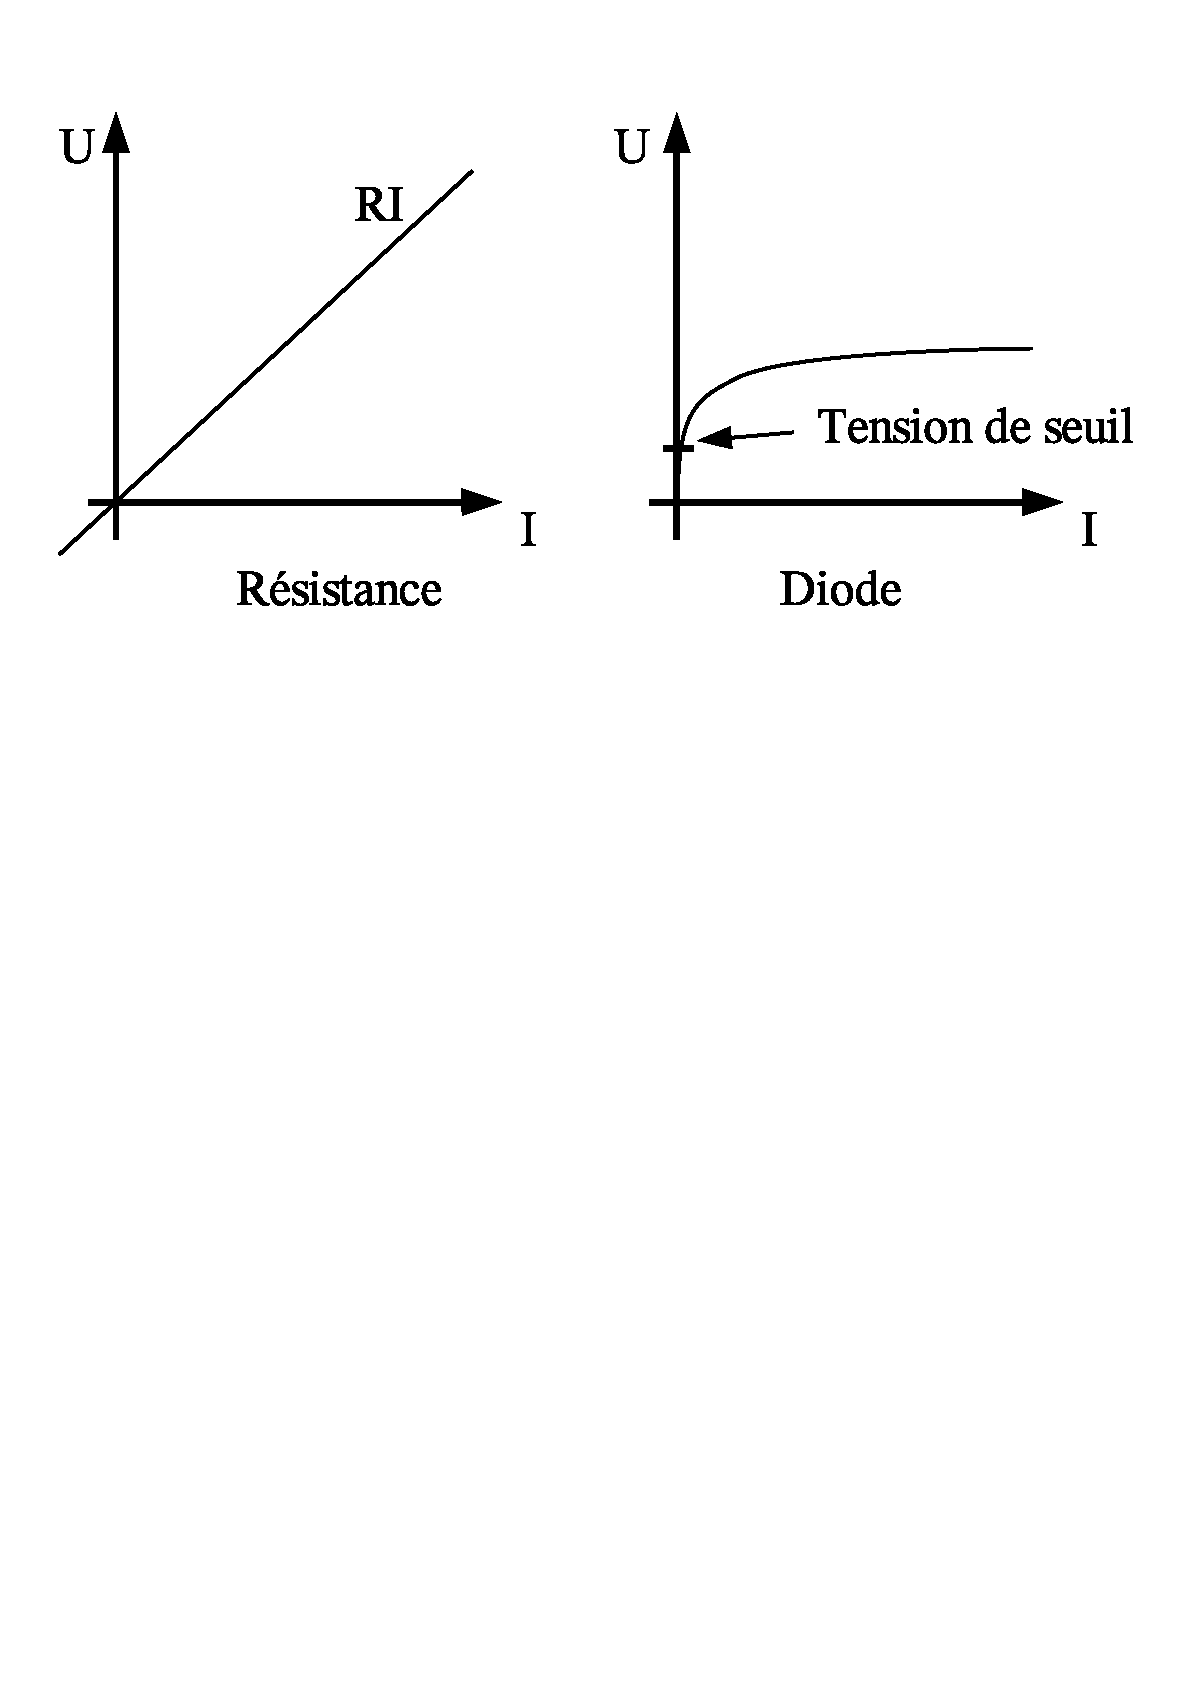
\includegraphics[clip=true,viewport=0cm 18cm 21cm 27cm,scale=0.75]{./figures/caracteristiques.pdf}
\caption{Exemples de caract�ristiques.}
\end{center}
\end{figure}

\subsubsection{Point de fonctionnement}

\begin{figure}[h]
\begin{center}
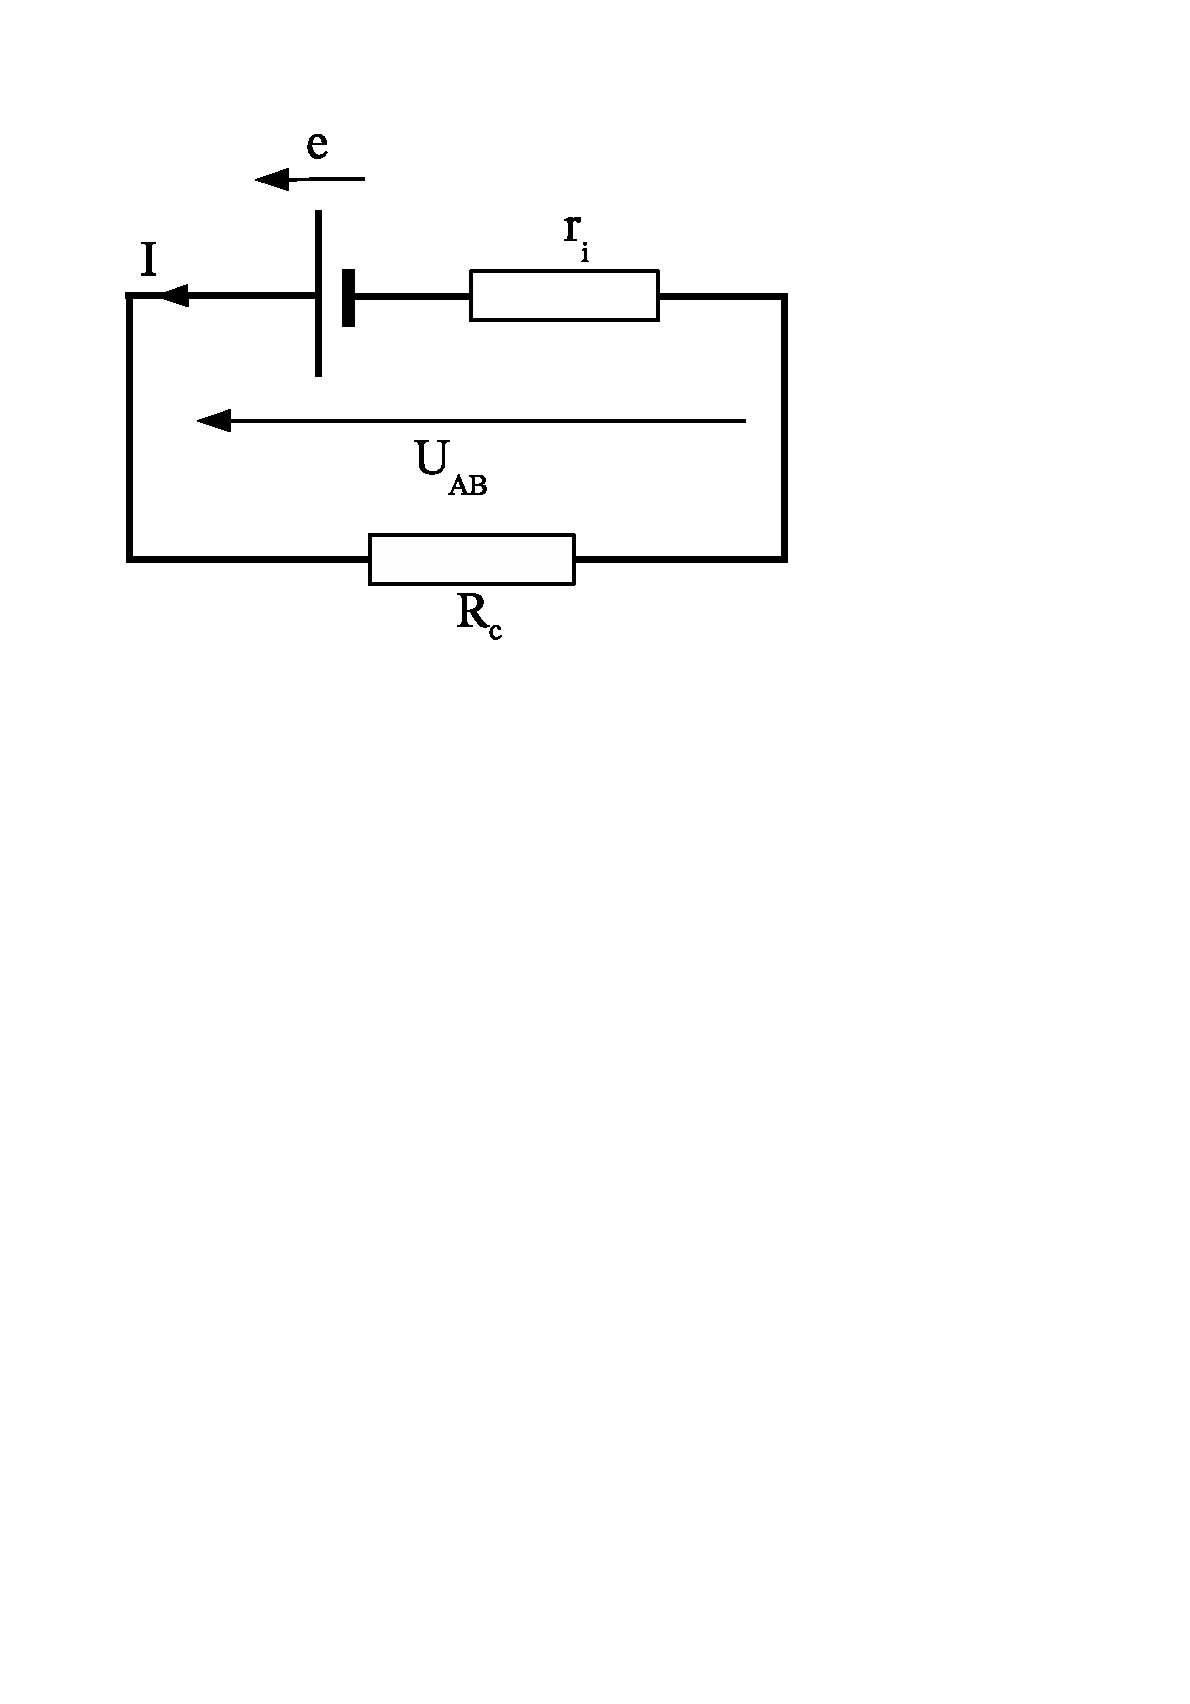
\includegraphics[clip=true,viewport=0cm 18cm 16cm 27cm,scale=0.5]{./figures/circuit.pdf}
\caption{Circuit �lectrique charg�}\label{circuit_01}
\end{center}
\end{figure}

Soit le circuit �lectrique donn� � la figure \ref{circuit_01}. Le courant s'�crit~:

$$I=\frac{e}{r_{i}+R_{c}}$$

d'o�

$$U_{AB}=e-r_{i}I=e-\frac{r_{i}e}{r_{i}+R_{c}}=\frac{e}{1+\frac{r_{i}}{R_{c}}}$$

Le \textbf{point de fonctionnement} est l'intersection des courbes $U_{AB}=e-r_{i}I=R_{c}I$ comme le montre la figure \ref{fig_pdf}

\begin{figure}[h]
\begin{center}
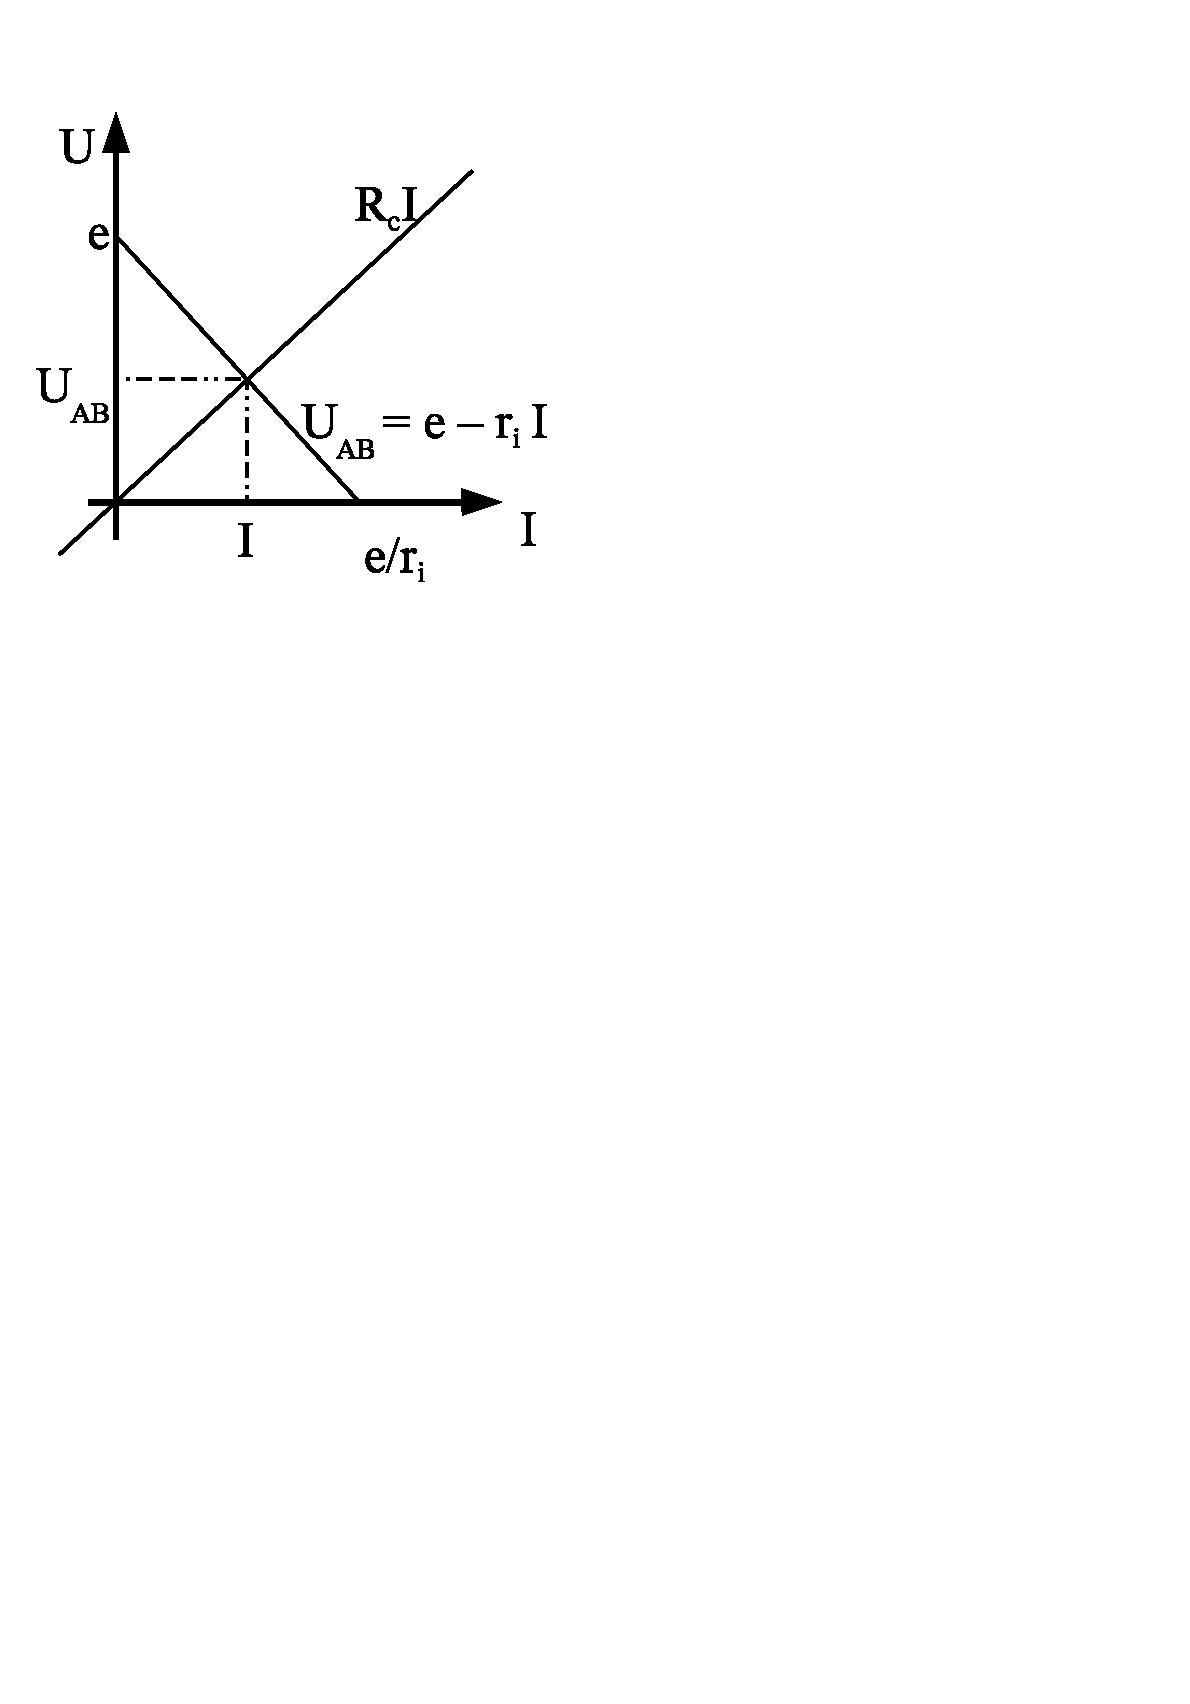
\includegraphics[clip=true,viewport=0cm 19cm 9.5cm 28cm,scale=0.7]{./figures/point_de_fonctionnement.pdf}
\caption{Point de fonctionnement.}\label{fig_pdf}
\end{center}
\end{figure}


\subsubsection{G�n�rateur de tension}

Si la r�sistance de charge $R_{c}$ est tr�s grande devant $r_{i}$, la tension aux bornes du g�n�rateur est sensiblement ind�pendante de $R_{c}$. On obtient alors un g�n�rateur � tension constante dont la courbe caract�ristique est donn�e � la figure \ref{fig_gen_ten}.

\begin{figure}[h]
\begin{center}
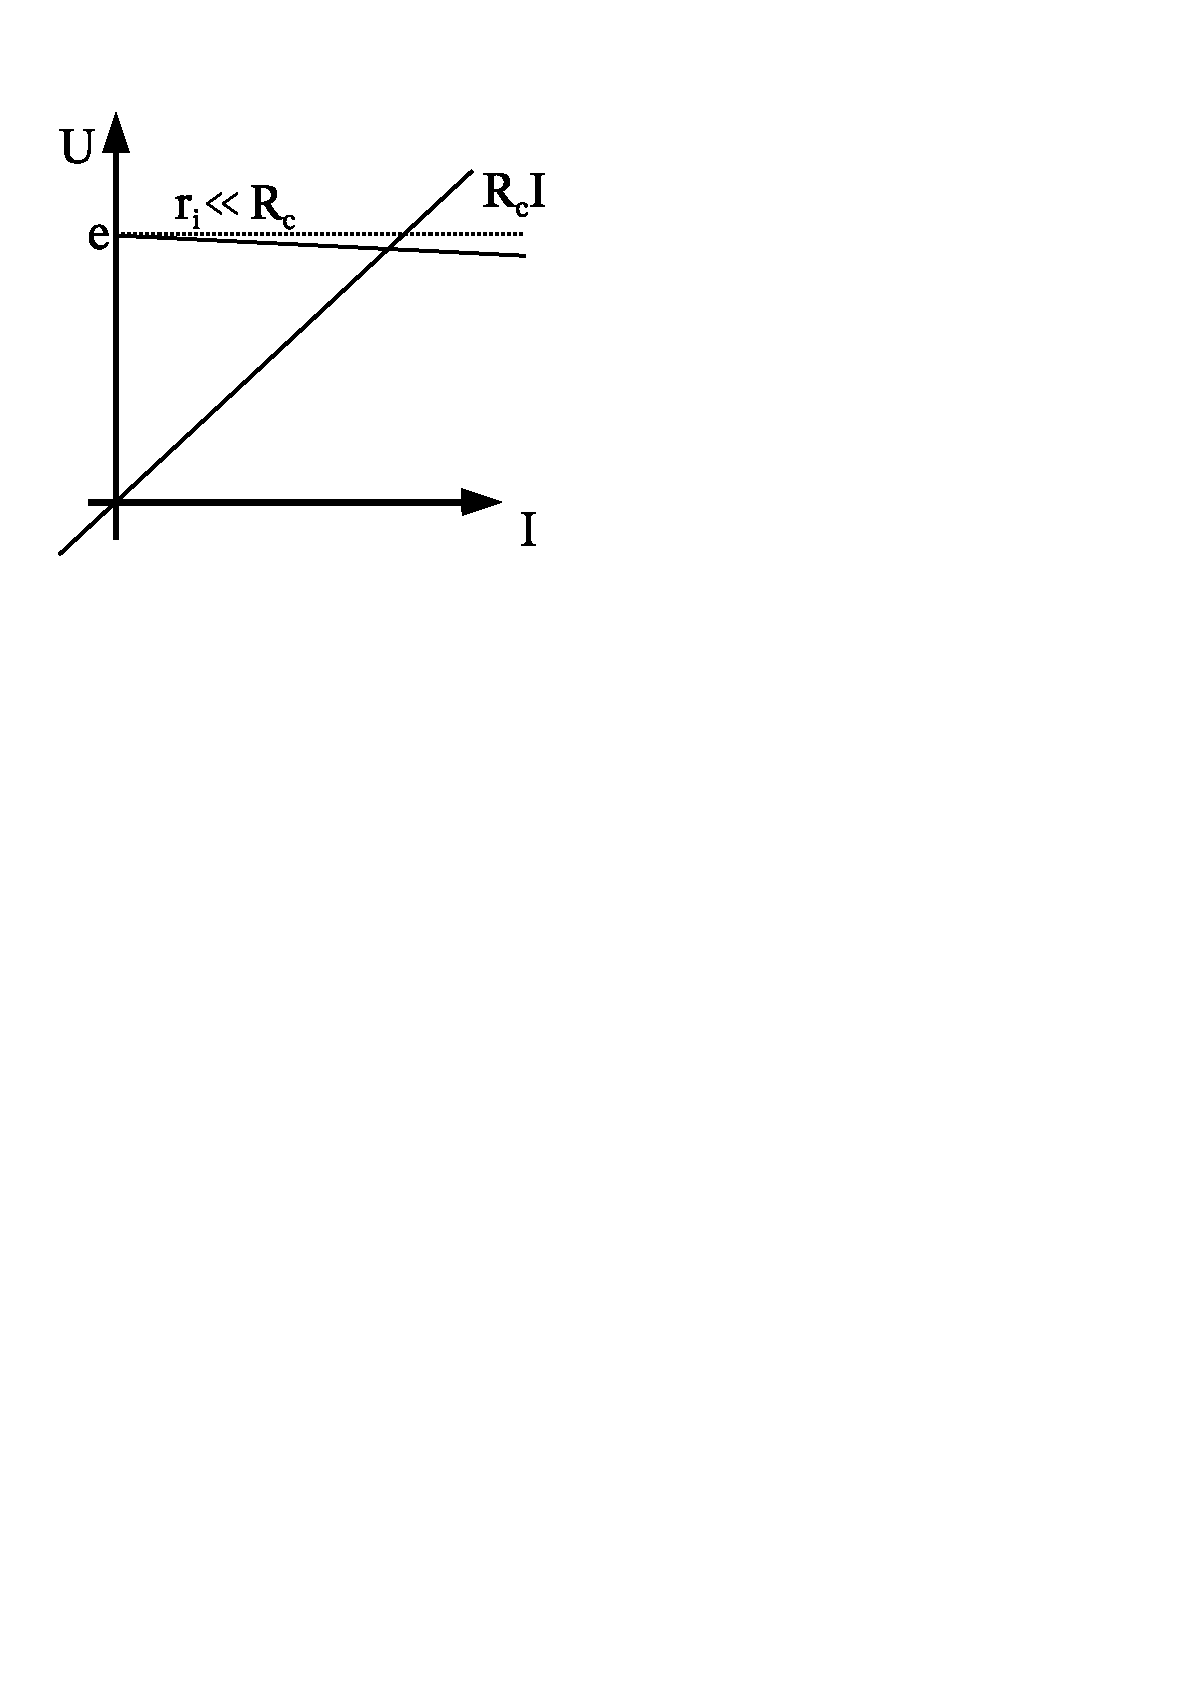
\includegraphics[clip=true,viewport=0cm 19cm 9.5cm 28cm,scale=0.6]{./figures/relation_tension_courant1.pdf}
\caption{Relation tension - courant $U=f(I)$ pour un g�n�rateur de tension.}\label{fig_gen_ten}
\end{center}
\end{figure}

On en d�duit~: $U = e - r_{i}I\approx e$.
Plus la r�sistance $r_{i}$ est petite, plus le g�n�rateur est capable de fournir un courant fort et plus la tension sera proche de $e$.


\subsubsection{G�n�rateur de courant}

Si la r�sistance de charge $R_{c}$ est tr�s petite devant $r_{i}$, alors $i=\fractext{e}{r_{i}+R_{c}}\approx \fractext{e}{r_{i}}$ est ind�pendant de la charge. On obtient alors un g�n�rateur de courant constant dont la courbe caract�ristique est donn�e � la figure \ref{fig_gen_cour}.

\begin{figure}[h]
\begin{center}
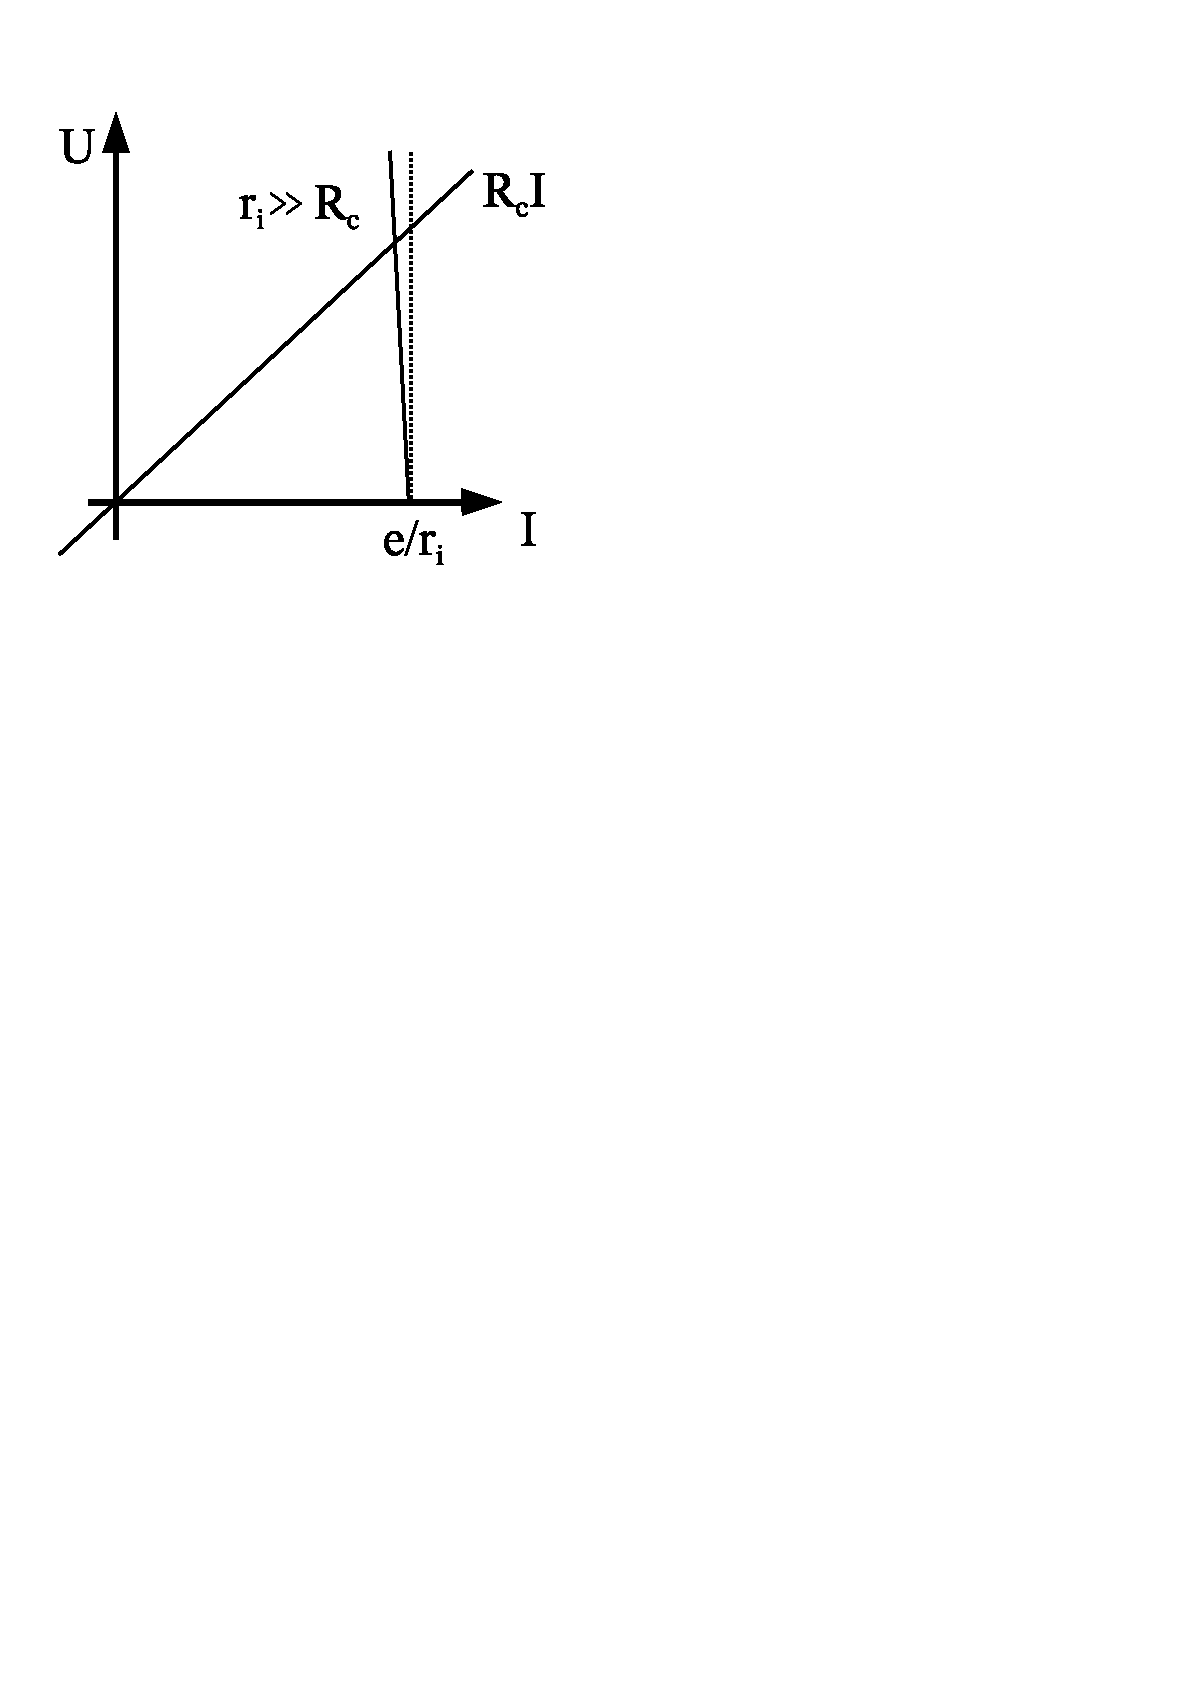
\includegraphics[clip=true,viewport=0cm 19cm 9.5cm 28cm,scale=0.6]{./figures/relation_tension_courant2.pdf}
\caption{Relation tension / courant~: $U=f(I)$ pour un g�n�rateur de courant.}\label{fig_gen_cour}
\end{center}
\end{figure}


\begin{figure}[h]
\begin{center}
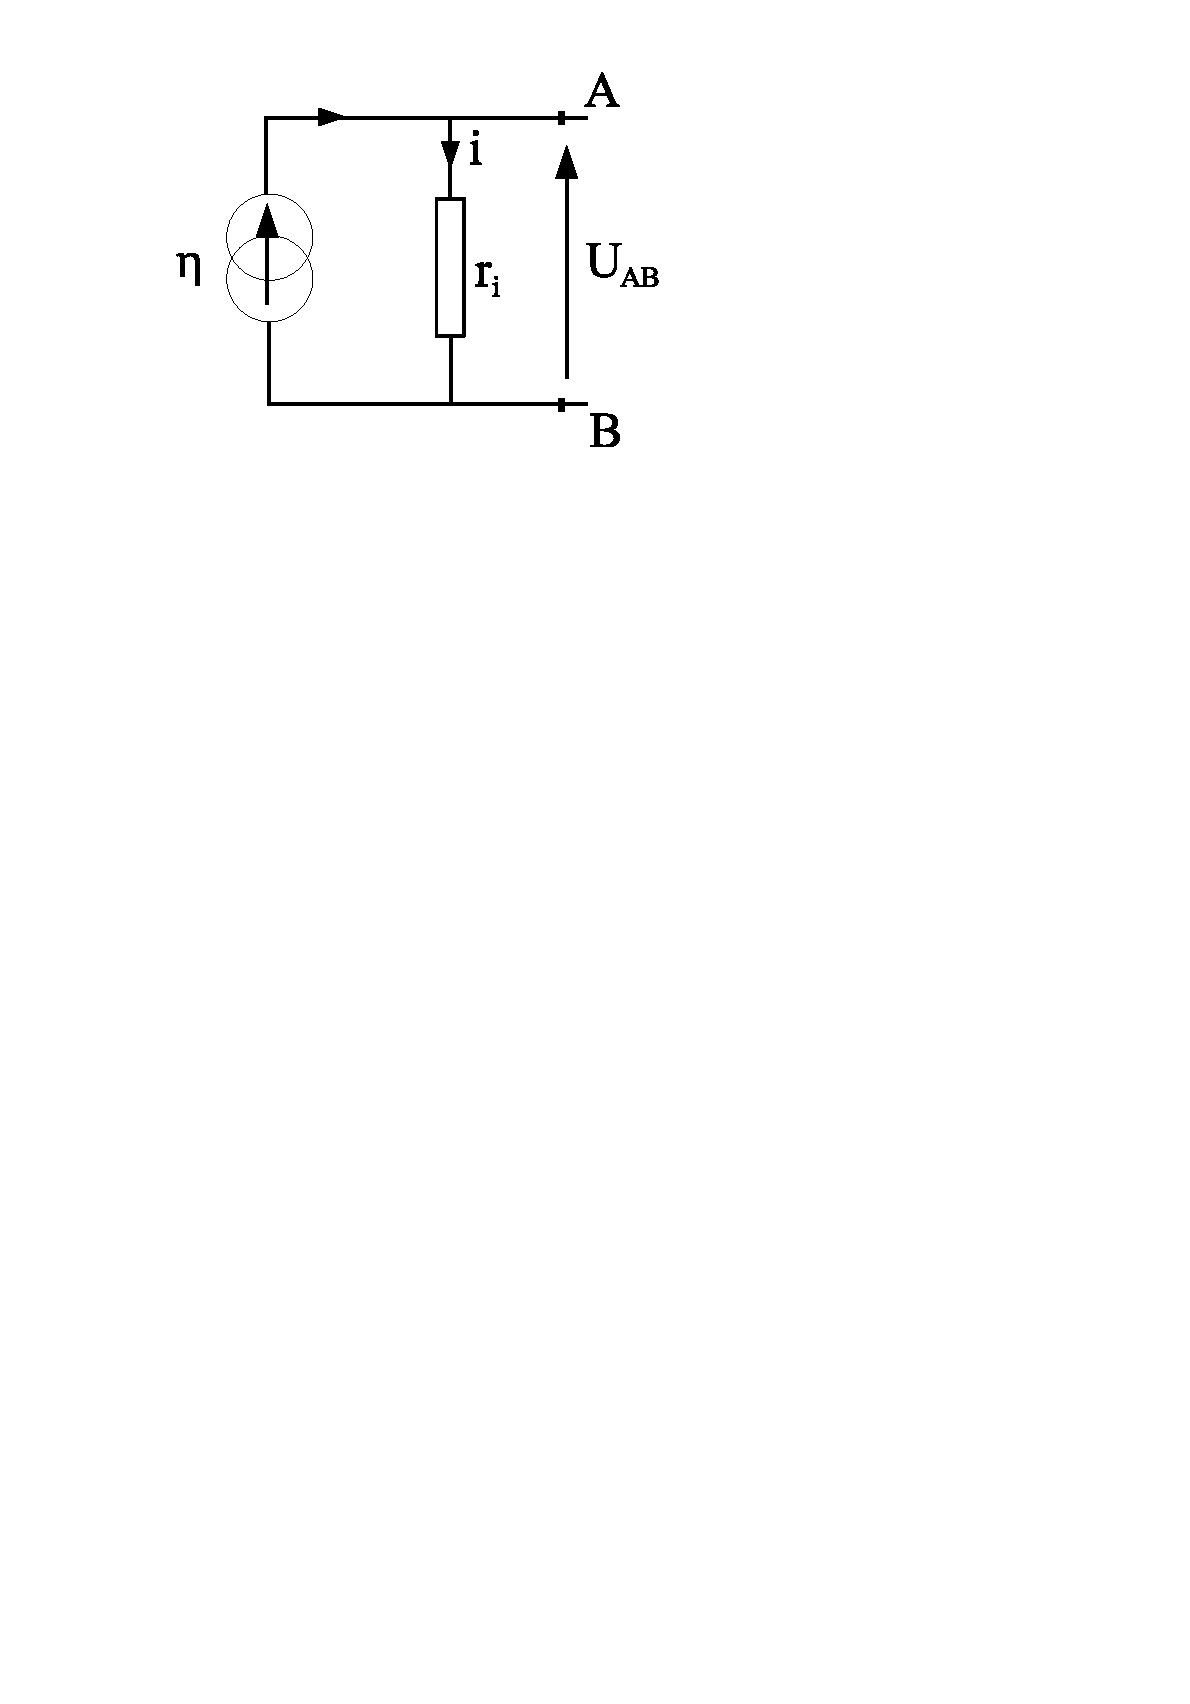
\includegraphics[clip=true,viewport=3cm 20cm 12cm 28cm,scale=0.6]{./figures/generateur_de_courant.pdf}
\caption{G�n�rateur de courant.}\label{sch_gen_cour}
\end{center}
\end{figure}

$\eta $ est le courant fournit par le g�n�rateur quand il y a court-circuit. En g�n�ral, l'imp�dance interne est une r�sistance $r_{i}$ d'o�~: $I = \eta  - \fractext{U}{r_{i}}$, avec $\eta = \fractext{e}{r_{i}}$.

Ici, plus la r�sistance est grande, plus le g�n�rateur est capable de d�livrer un courant proche de $\eta $. La symbolique utilis�e pour sch�matiser ce type de g�n�rateur est pr�sent�e � la figure \ref{sch_gen_cour}.


\subsubsection{Repr�sentation Duale}
L'�quivalence entre les deux repr�sentations est appel�e \textbf{dualit�}. En effet, on peut �crire � la fois :

$$U = e - r_{i} I$$

et

$$I = \frac{e}{r_{i}}-\frac{U}{r_{i}}=\eta  - g_{i}U$$

en posant $\eta =\fractext{e}{r_{i}}$ et $g_{i}=\fractext{1}{r_{i}}$. $e$ et $\eta $ sont orient�s dans le m�me sens. Le principe de dualit� sch�matis� est donn� � la figure \ref{sch_dual}.

\begin{figure}[h]
\begin{center}
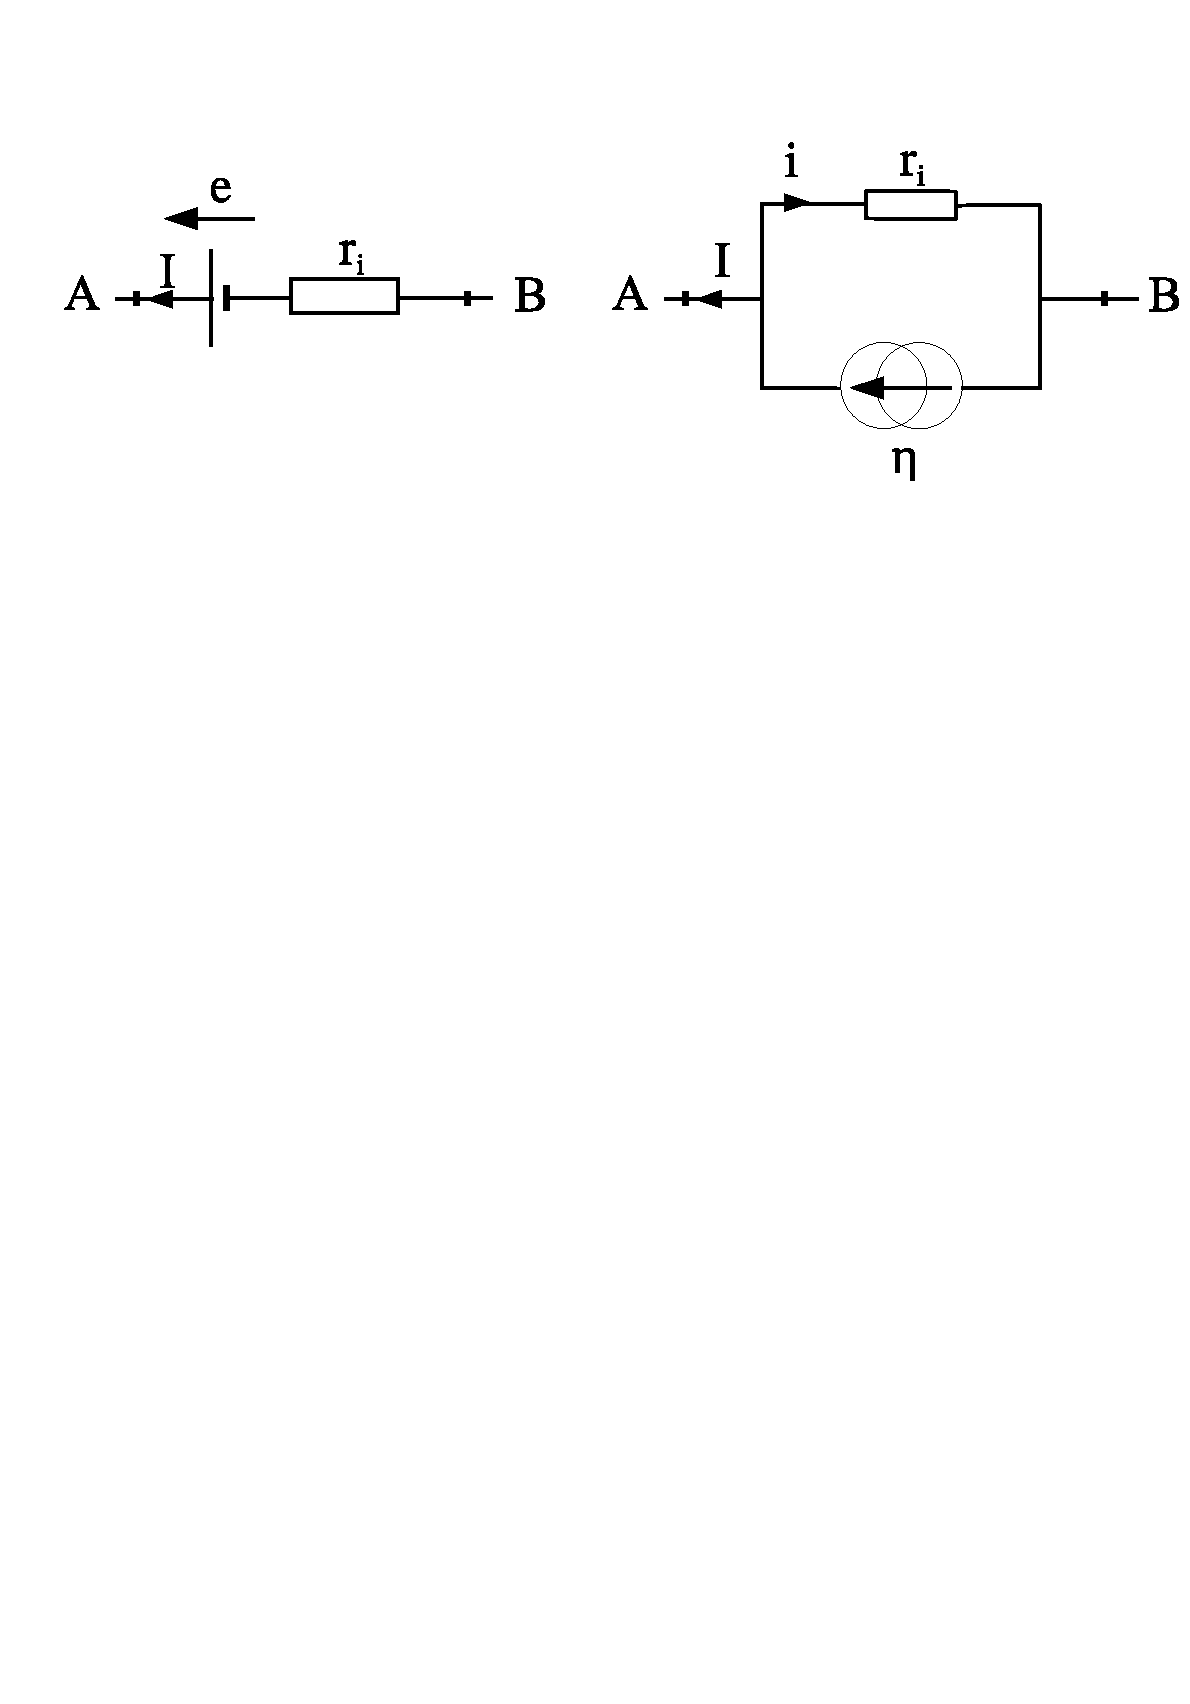
\includegraphics[clip=true,viewport=0cm 20cm 21cm 27cm,scale=0.5]{./figures/representation_duale.pdf}
\caption{Dualit� g�n�rateurs de tension / courant.}\label{sch_dual}
\end{center}
\end{figure}

\begin{itemize}
 \item  G�n�rateur de tension~:

$$U_{AB}=R_{c} I$$
$$I = \frac{E}{R_{i}+R_{c}}$$
$$U_{AB}=\frac{R_{c}}{R_{i}+R_{c}} E$$

 \item G�n�rateur de courant~:

$$\eta =I+i$$
$$I=\eta - \frac{U_{AB}}{r_{i}} I$$
$$I(1+\frac{R_{c}}{r_{i}})=\eta$$
$$I=\frac{r_{i}}{r_{i}+R_{c}} \eta$$

$$I = \frac{1}{r_{i}+R_{c}} e$$
$$U_{AB}=R_{c} I$$
$$U_{AB}=\frac{R_{c}}{R_{i}+R_{c}} E$$
\end{itemize}

On peut r�sumer l'effet de la dualit� ainsi : quand un g�n�rateur de f�m $E$ et de r�sistance interne $R_{i}$ d�bite dans une r�sistance de charge $R_{c}$~:

\begin{itemize}
\item si $r_{i} \ll R_{c}$, alors c'est une source de tension de f�m $E$ ;
\item si $r_{i} \gg R_{c}$, alors c'est une source de courant $I = \fractext{e}{r_{i}}$.
\end{itemize}


\subsubsection{Associations de dip�les~: dip�les �quivalents}

\begin{itemize}
\item Association en s�rie~:

Tension~: $u = \sum_{k} u_{k}$ (somme alg�brique sur une branche)
Source de tension~: $e = \sum_{k} e_{k}$ (somme alg�brique)
R�sistance~: $R = \sum_{k} R_{k}$

De mani�re g�n�rale~: $u = \sum_{k} u_{k} = \sum_{k} e_{k} + (\sum_{k} R_{k}) I$.

\begin{note}L'association en s�rie de sources de courant id�ale n'a aucun sens.
\end{note}

\item Association en parall�le~:

Courant~: $I = \sum_{k} I_{k}$ (somme alg�brique � un n\oe ud)
Conducteur ohmique~: $G = \sum_{k} G_{k}$ (conductance �quivalente)

De mani�re g�n�rale~: $i = \sum_{k} i_{k} = \sum_{k} \eta_{k} + (\sum_{k} G_{k}) U$.

\begin{note} L'association en parall�le de sources de tension id�ales n'a aucun sens.
\end{note}

\end{itemize}


\subsubsection{Adaptation d'imp�dance~: charge adapt�e}

Soit un g�n�rateur de tension dans une r�sistance $R_{c}$.

\begin{figure}[h]
\begin{center}
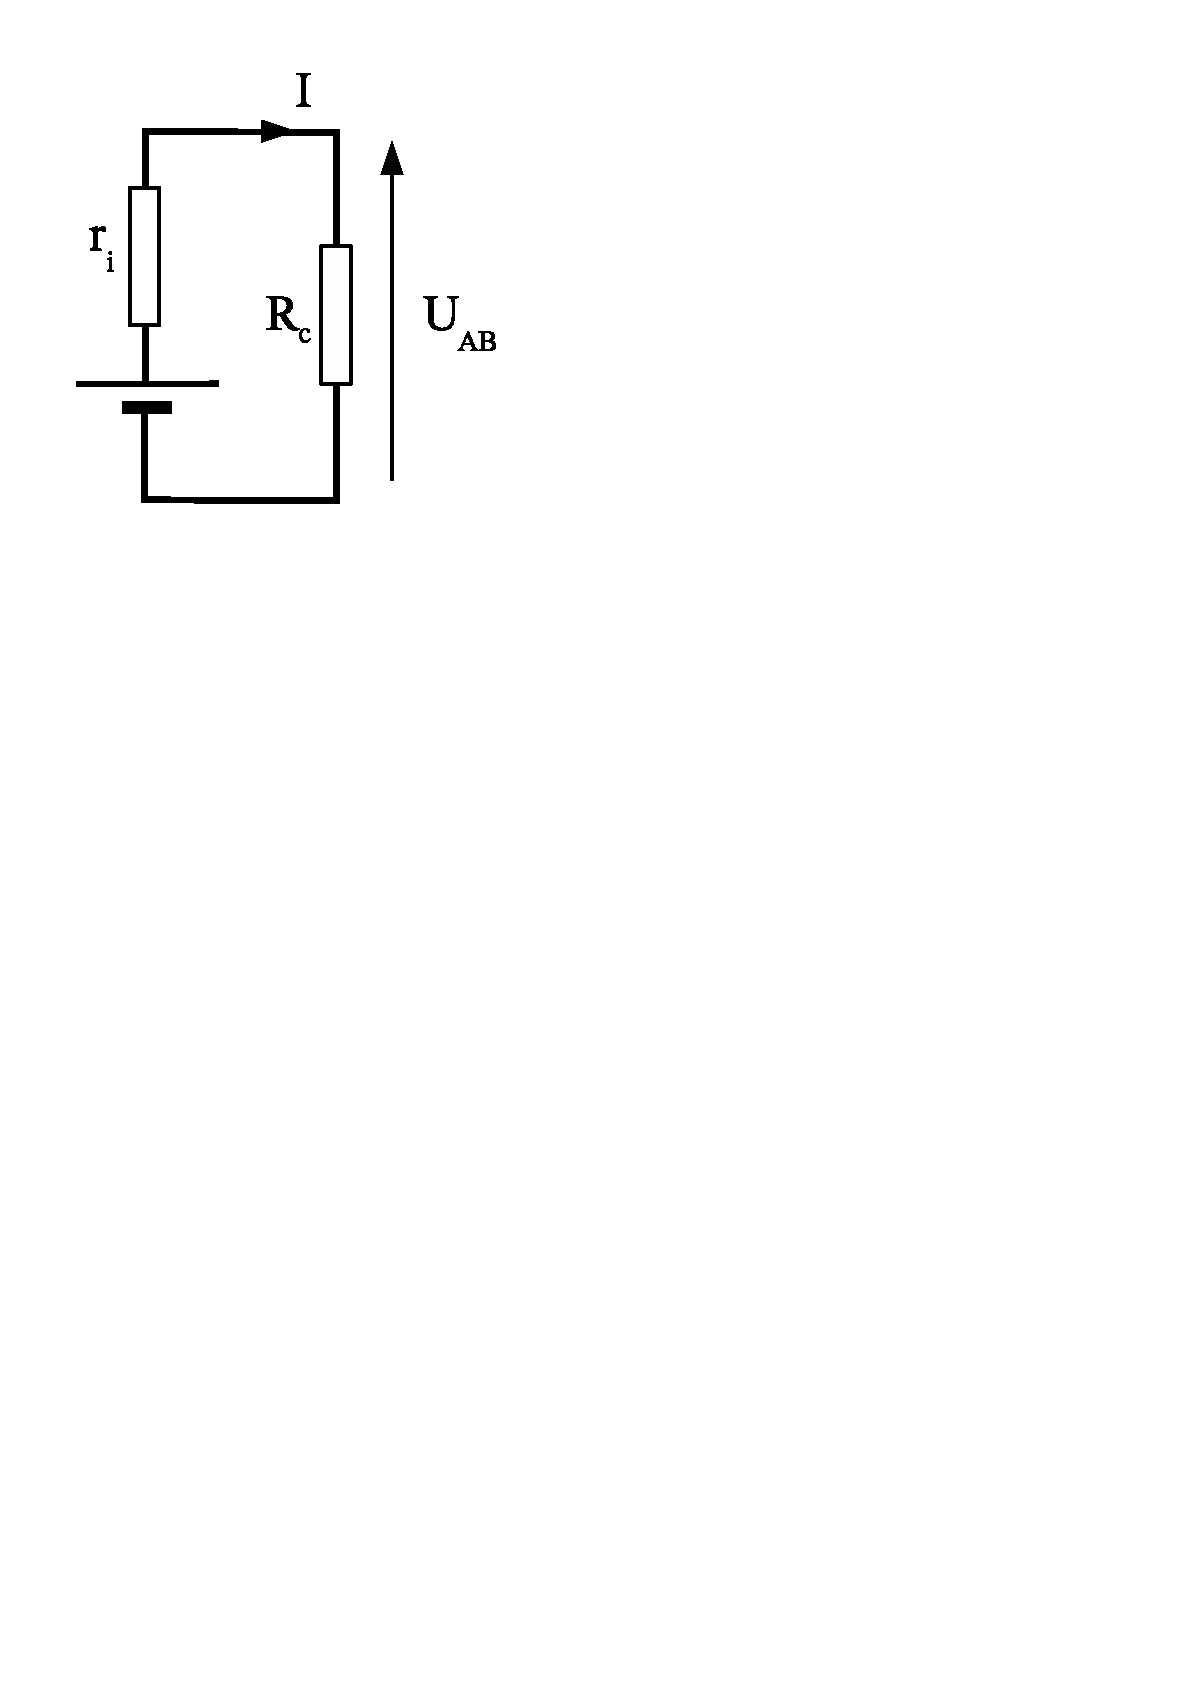
\includegraphics[clip=true,viewport=0cm 20cm 10cm 27cm,scale=0.38]{./figures/circuit_charge.pdf}
\caption{G�n�rateur de tension charg�.}
\end{center}
\end{figure}

$$ \left\{
\begin{array}{ll}
U_{AB}=e-r_{i}I \\
U_{AB}=R_{c} I
\end{array} \right.
$$

$$U_{AB}=e-\frac{r_{i}}{R_{c}} U_{AB}$$

$$e = \frac{R_{c}+r_{i}}{R_{c}} U_{AB}$$

$$U_{AB} = \frac{R_{c}}{R_{c}+r_{i}} e \qquad \textrm{et} \qquad I=\fractext{e}{R_{c}+r_{i}}$$


\begin{description}

\item[Puissance dissip�e dans $r_{i}$]
$$P_{c}=UI=r_{i} I^{2}$$

Nous avons~:
$$P_{c}=\frac{r_{i}}{(R_{c}+r_{i})^2} e^{2}$$

\item[Puissance dissip�e dans $R_ {c}$]
$$P_{c}=U_{AB}I=R_{c} I^{2}$$
avec $I=\fractext{e}{R_{c}+r_{i}}$.

Nous avons~:
$$P_{c}=\frac{R_{c}}{(R_{c}+r_{i})^2} e^{2}$$


Quelle doit �tre la r�sistance de charge pour que la puissance soit maximale ?

\begin{figure}[h]
\begin{center}
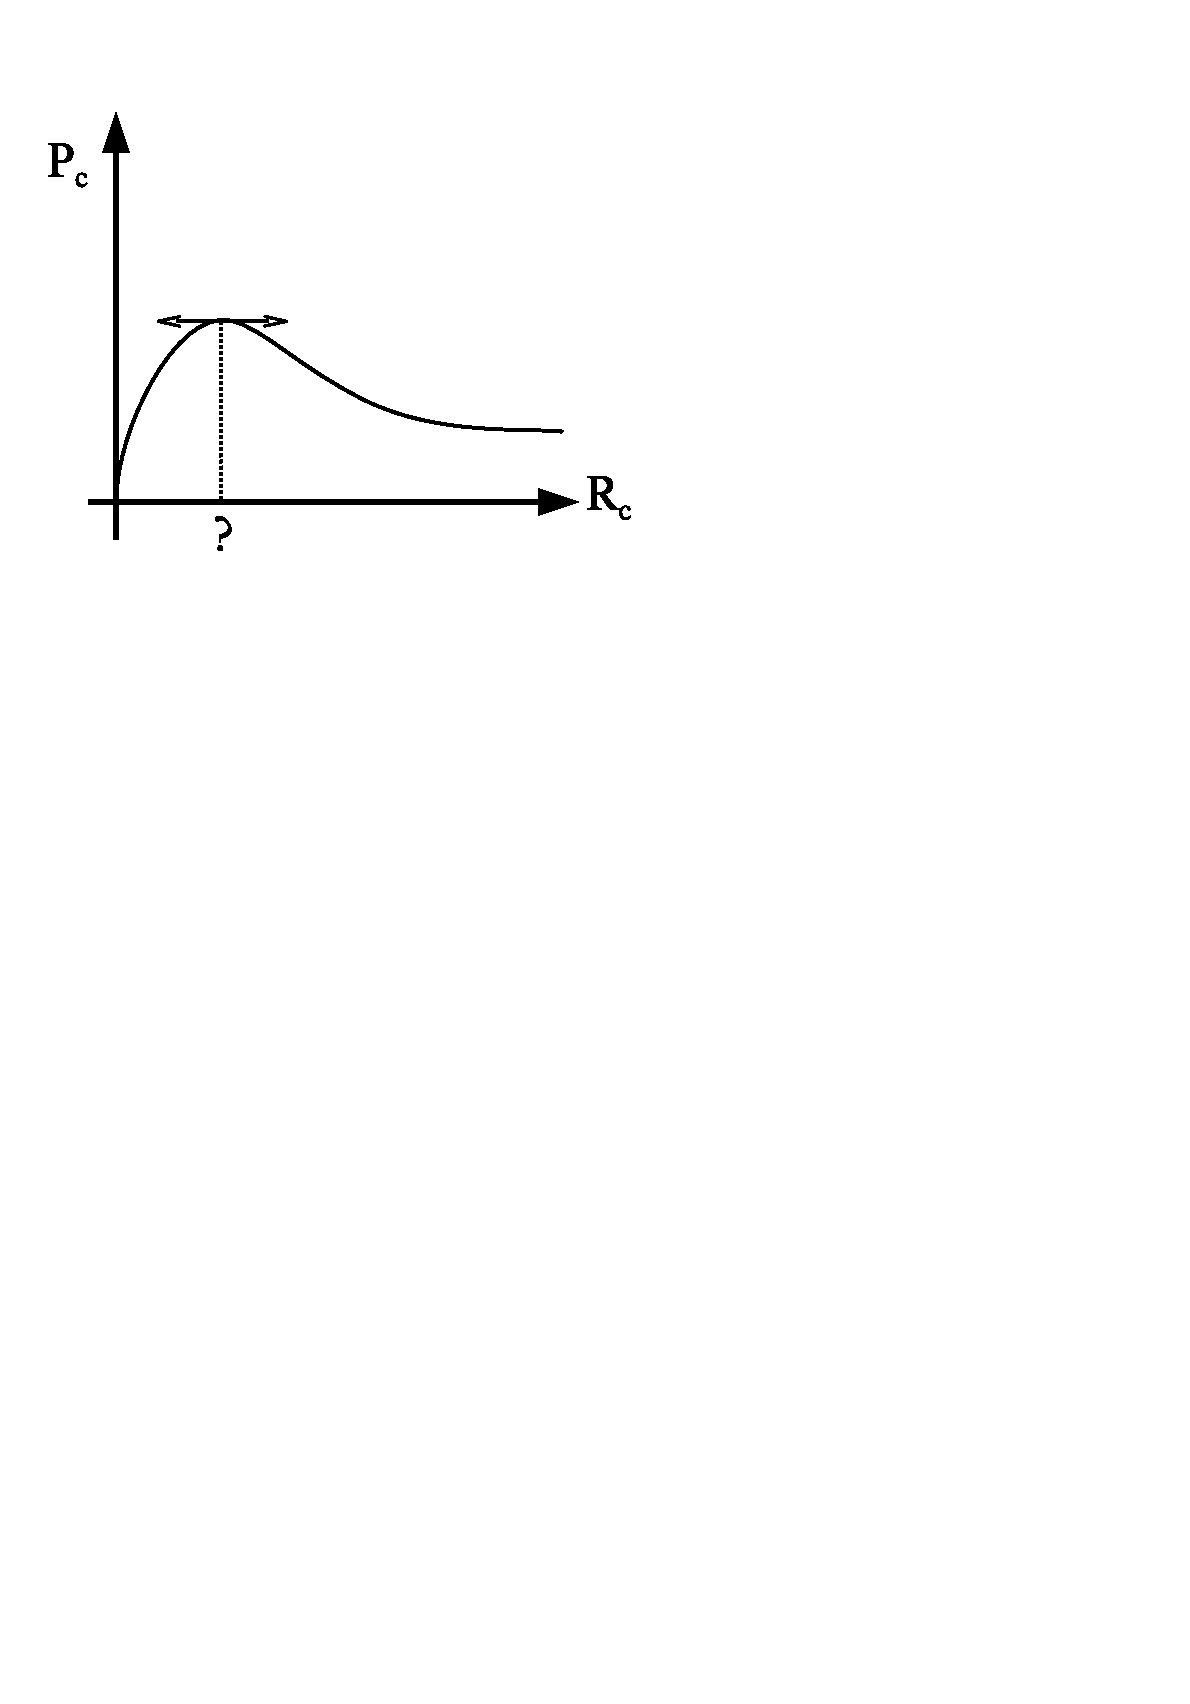
\includegraphics[clip=true,viewport=0cm 18cm 12cm 27cm,scale=0.5]{./figures/puissance_fournie.pdf}
\caption{Puissance fournie.}
\end{center}
\end{figure}

$Pc$ est maximum lorsque $\fractext{\partial P_{c}}{\partial R_{c}}=0$, soit~:

\begin{equation*}
\begin{split}
\frac{\partial P_{c}}{\partial R_{c}} & = \frac{R_{c}+R_{i}-2R_{c}}{(R_{c}+r_{i})^{3}} e^{2} \\
& = \frac{R_{c}+r_{i}-2R_{c}}{(R_{c}+r_{i})^{3}} e^{2}
\end{split}
\end{equation*}

donc lorsque $R_{i}=R_{c}$.
\bigskip

\item[Puissance totale]
$$P_{tot}=eI=P_{c}+P_{i}=\frac{e^{2}}{R_{c}+r_{i}}$$
\end{description}


\section{R�seaux �lectriques}


\subsection{Analyse d'un r�seau en r�gime continu - M�thode de Kirchhoff}

L'analyse d'un r�seau consiste � d�terminer l'intensit� du courant qui circule dans chacune des branches ou des diff�rences de potentiel de chaque branche.

\begin{itemize}
\item Si il y a $N$ n\oe uds, il y a $N-1$ �quations de n\oe uds.
\item Si il y a $B$ branches, il y a $B-(N-1)$ �quations des mailles.
\item On cherche $B$ intensit�s.
\end{itemize}

\begin{enumerate}
\item Fl�cher arbitrairement les courants dans les diff�rentes branches, puis les diff�rences de potentiel. On choisi ensuite un sens arbitraire de description de chacune des mailles.
\item Appliquer la loi des n\oe uds.
Il n'y a pas d'accumulations de charges �lectriques � un n\oe ud, ce qui implique que la somme alg�brique des intensit�s des branches connect�es � un n\oe ud est nulle.

\begin{figure}[h]
\begin{center}
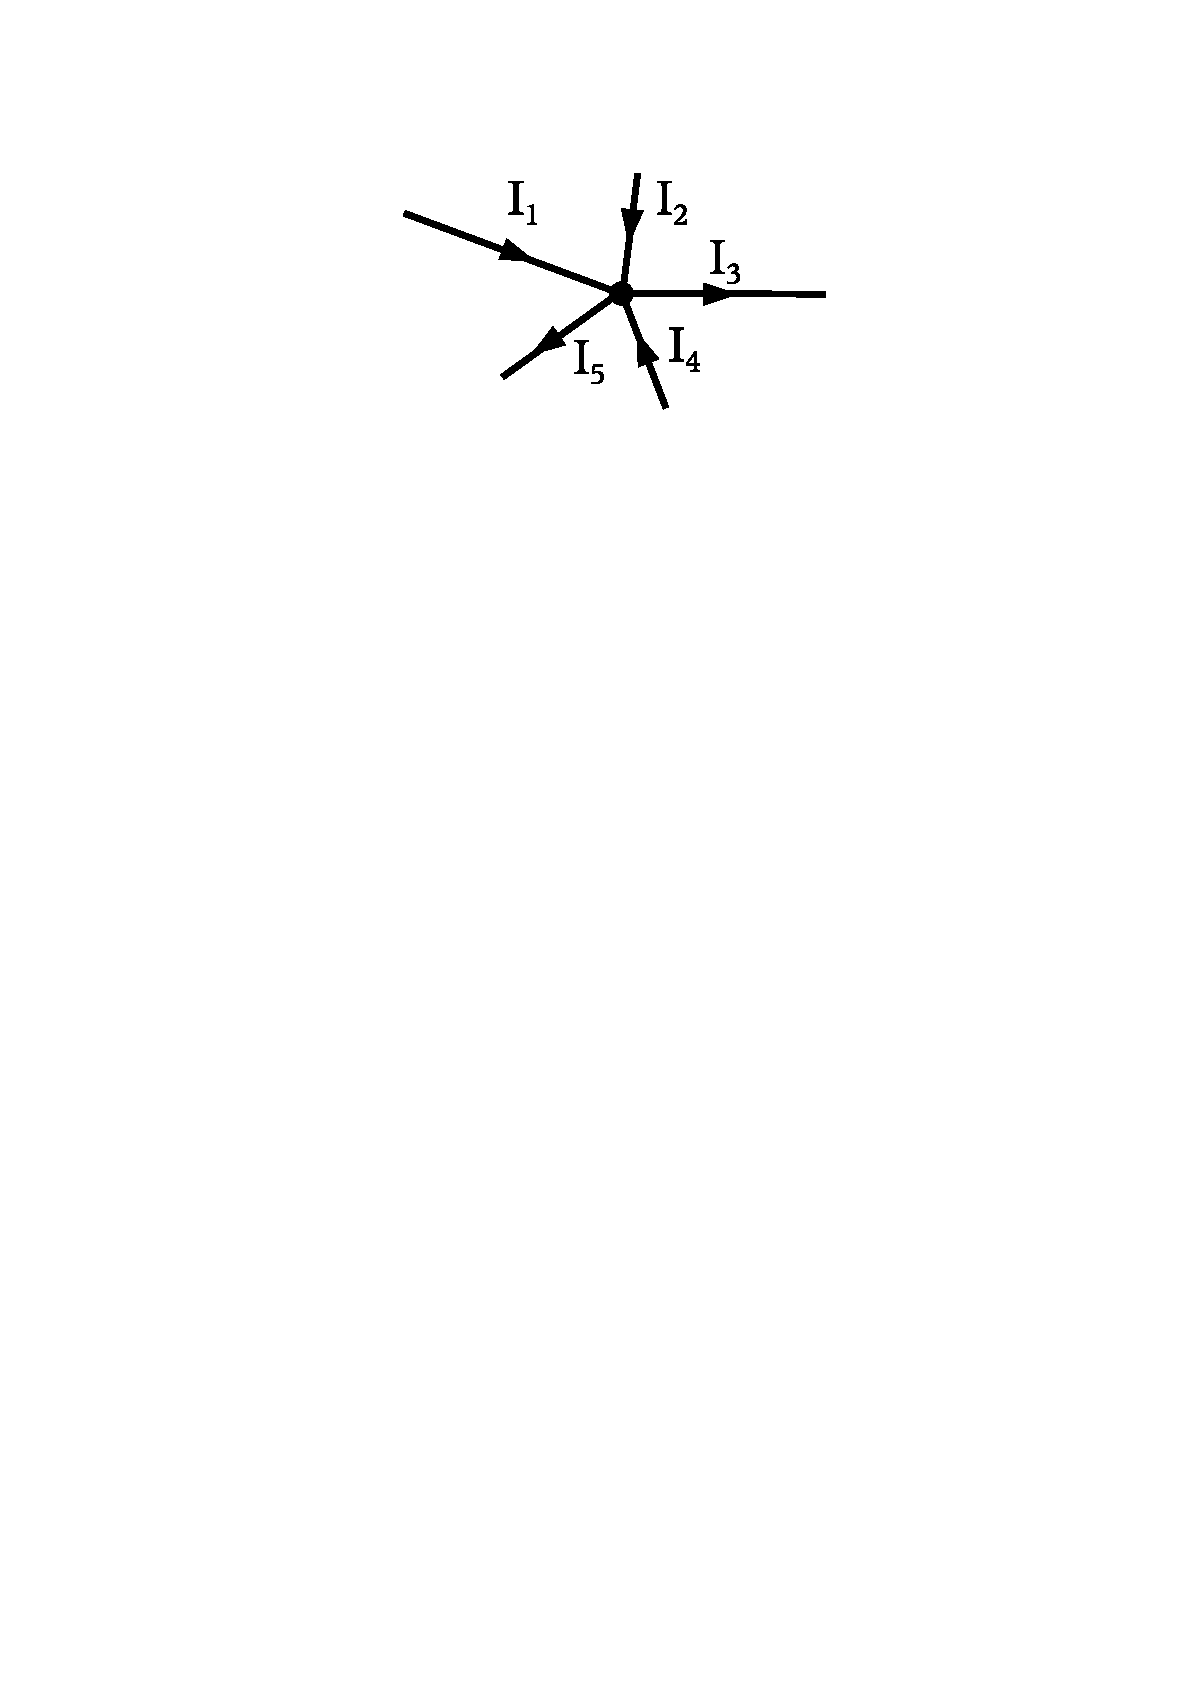
\includegraphics[clip=true,viewport=0cm 22cm 20cm 26cm,scale=0.38]{./figures/loi_des_noeuds.pdf}
\caption{Loi des n\oe uds.}
\end{center}
\end{figure}

$$\sum_{i} I = 0$$

On peut prendre comme convention $+$ si le courant va vers le n\oe ud et $-$ si il en sort.

\item Appliquer la loi des mailles.
En parcourant compl�tement une maille, la somme des diff�rences de potentiels rencontr�s est nulle : $V_{A} - V_{A}$.


\begin{figure}[h]
\begin{center}
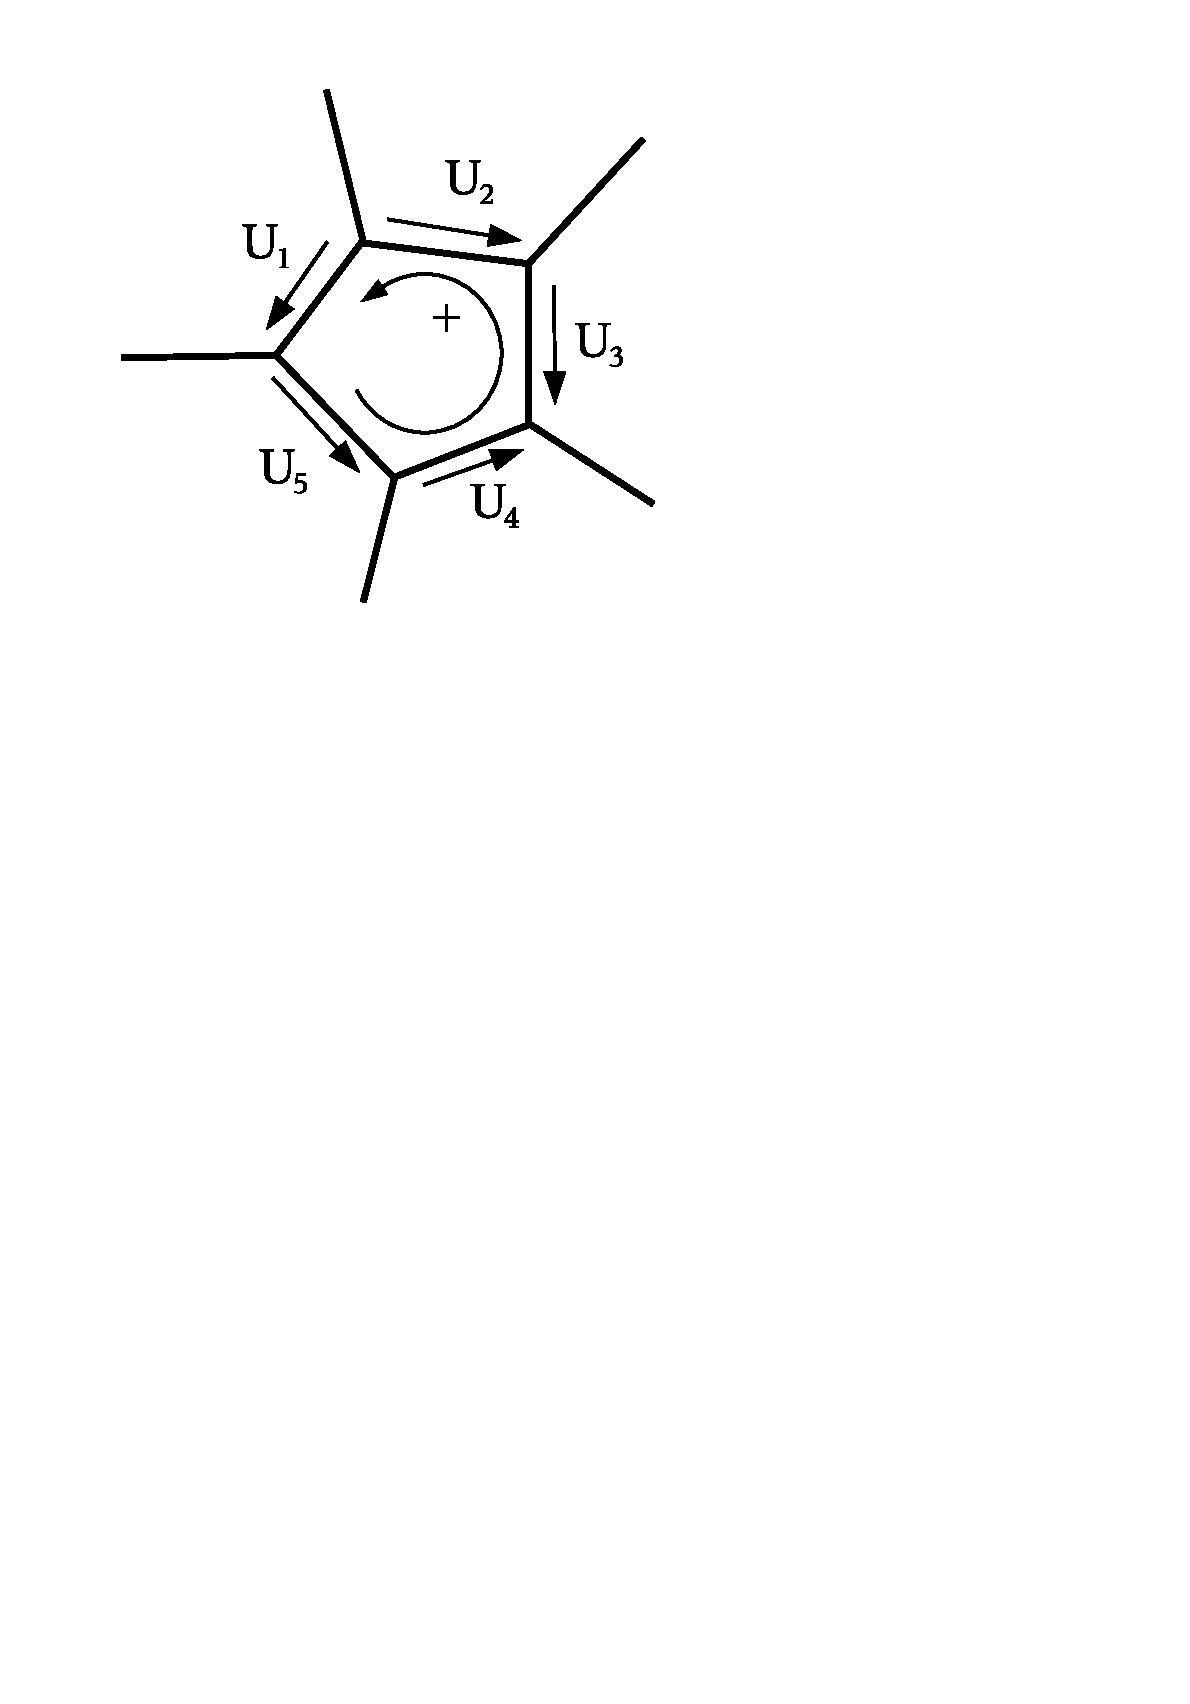
\includegraphics[clip=true,viewport=0cm 18.5cm 18cm 27.5cm,scale=0.55]{./figures/loi_des_mailles.pdf}
\caption{Loi des mailles.}
\end{center}
\end{figure}

$$U_{1}-U_{2}-U_{3}+U_{4}+U_{5}=0.$$


\item R�solution.
Les $B$ �quations obtenues � $B$ inconnues sont r�solues par m�thodes classiques (substitution, d�terminant, ...). Nous obtenons alors des valeurs alg�briques des courants~:
si $I_{i} >0$~: le sens choisi �quivaut au sens r�el ;
si $I_{i} >0$~: le sens choisi est inverse au sens r�el.

\end{enumerate}

\subsection{M�thode de superposition}
Le courant produit dans une branche quelconque d'un r�seau, par un ensemble de sources, est la somme alg�brique des courants produits dans chaque branche par chacune des sources consid�r�es isol�ment, les autres sources �tant rendues passives.
Rendre passives les sources signifit annuler les f�m (court-circuit�es) et les courants �lectromoteurs (circuits ouverts).

Exemple~:

\begin{figure}[h]
\begin{center}
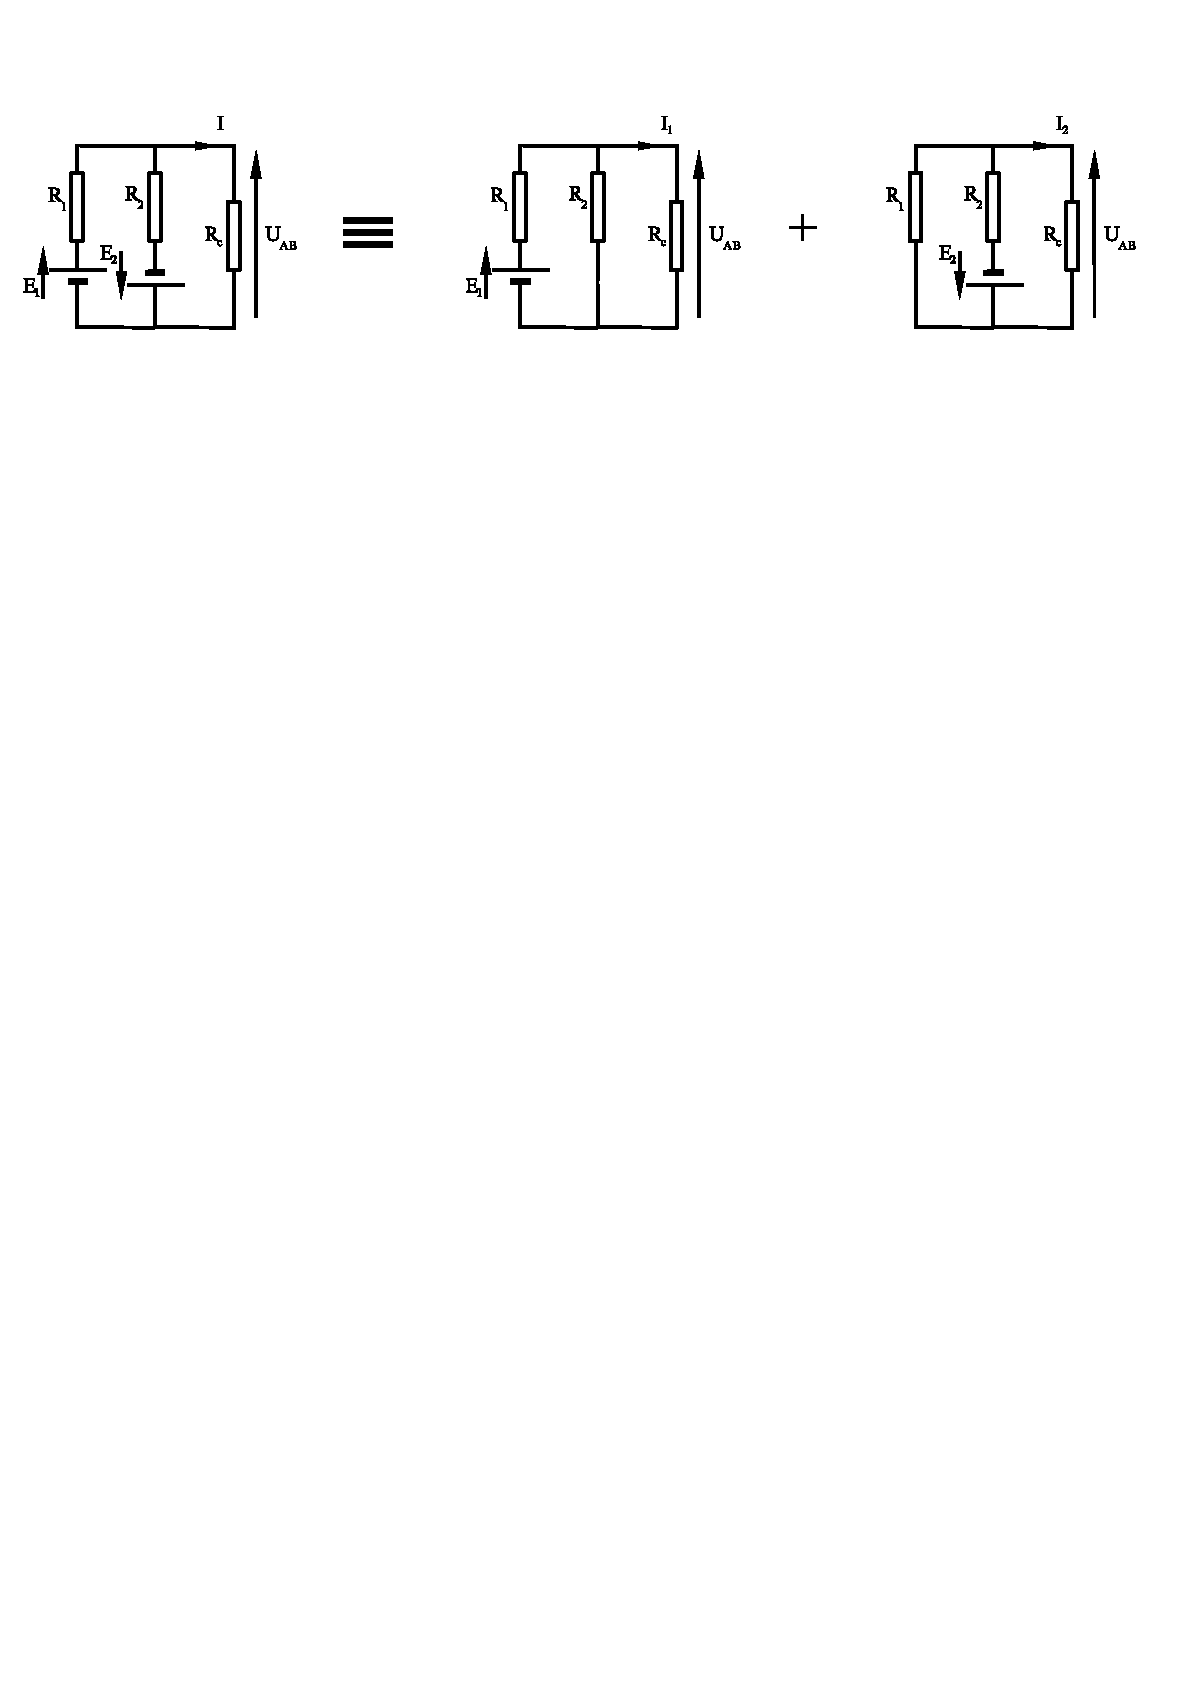
\includegraphics[clip=true,viewport=0cm 23cm 20cm 27cm,scale=0.9]{./figures/methode_superposition.pdf}
\caption{M�thodes de superposition.}
\end{center}
\end{figure}

\subsection{Th�or�me de Millmann}

Ce th�or�me s'applique dans le cas de branche en parall�le.

\begin{figure}[h]
\begin{center}
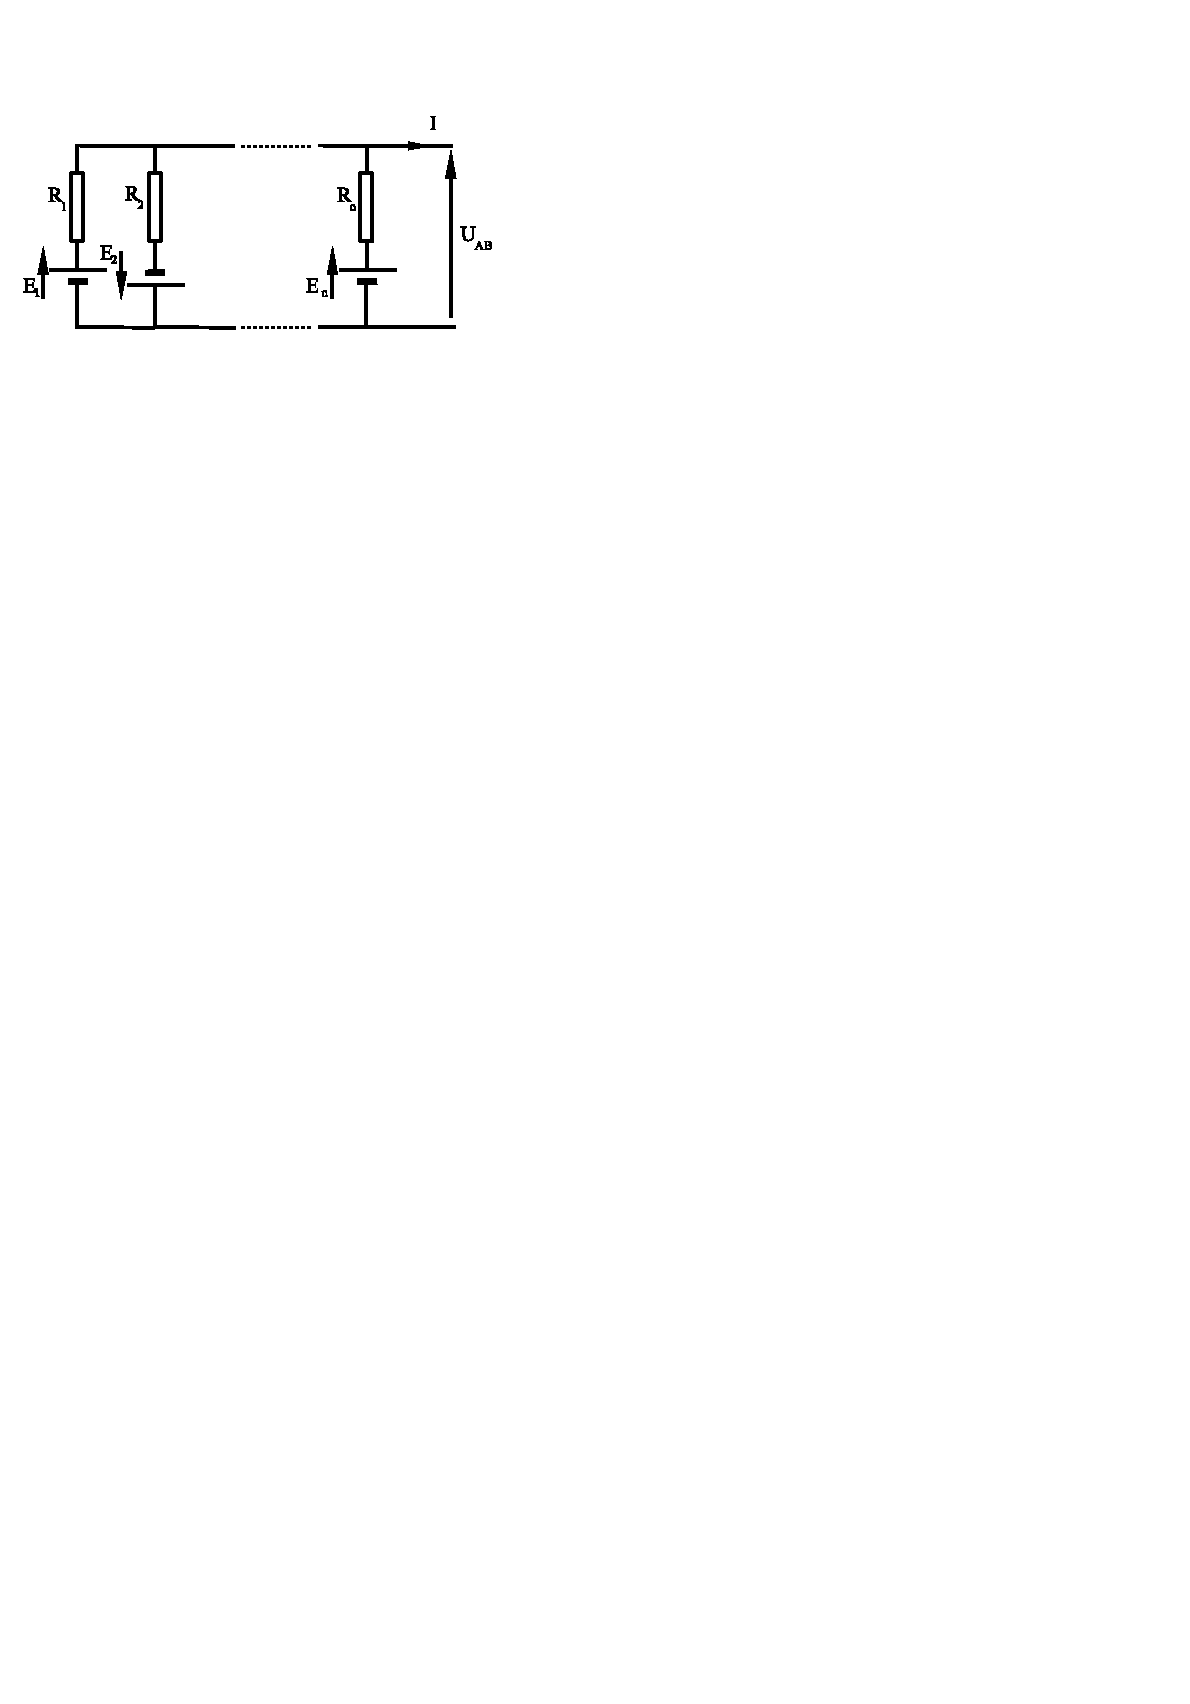
\includegraphics[clip=true,viewport=0cm 23cm 9cm 27cm,scale=1]{./figures/methode_millmann.pdf}
\caption{Th�or�me de Millmann.}
\end{center}
\end{figure}

$$U_{AB} = \fractext{\sum_{i} \pm \fractext{e_{i}}{r_{i}}} {\sum_{i} \fractext{1}{r_{i}}}.$$

La d�monstration par dualit� est �vidente~:

\begin{figure}[h]
\begin{center}
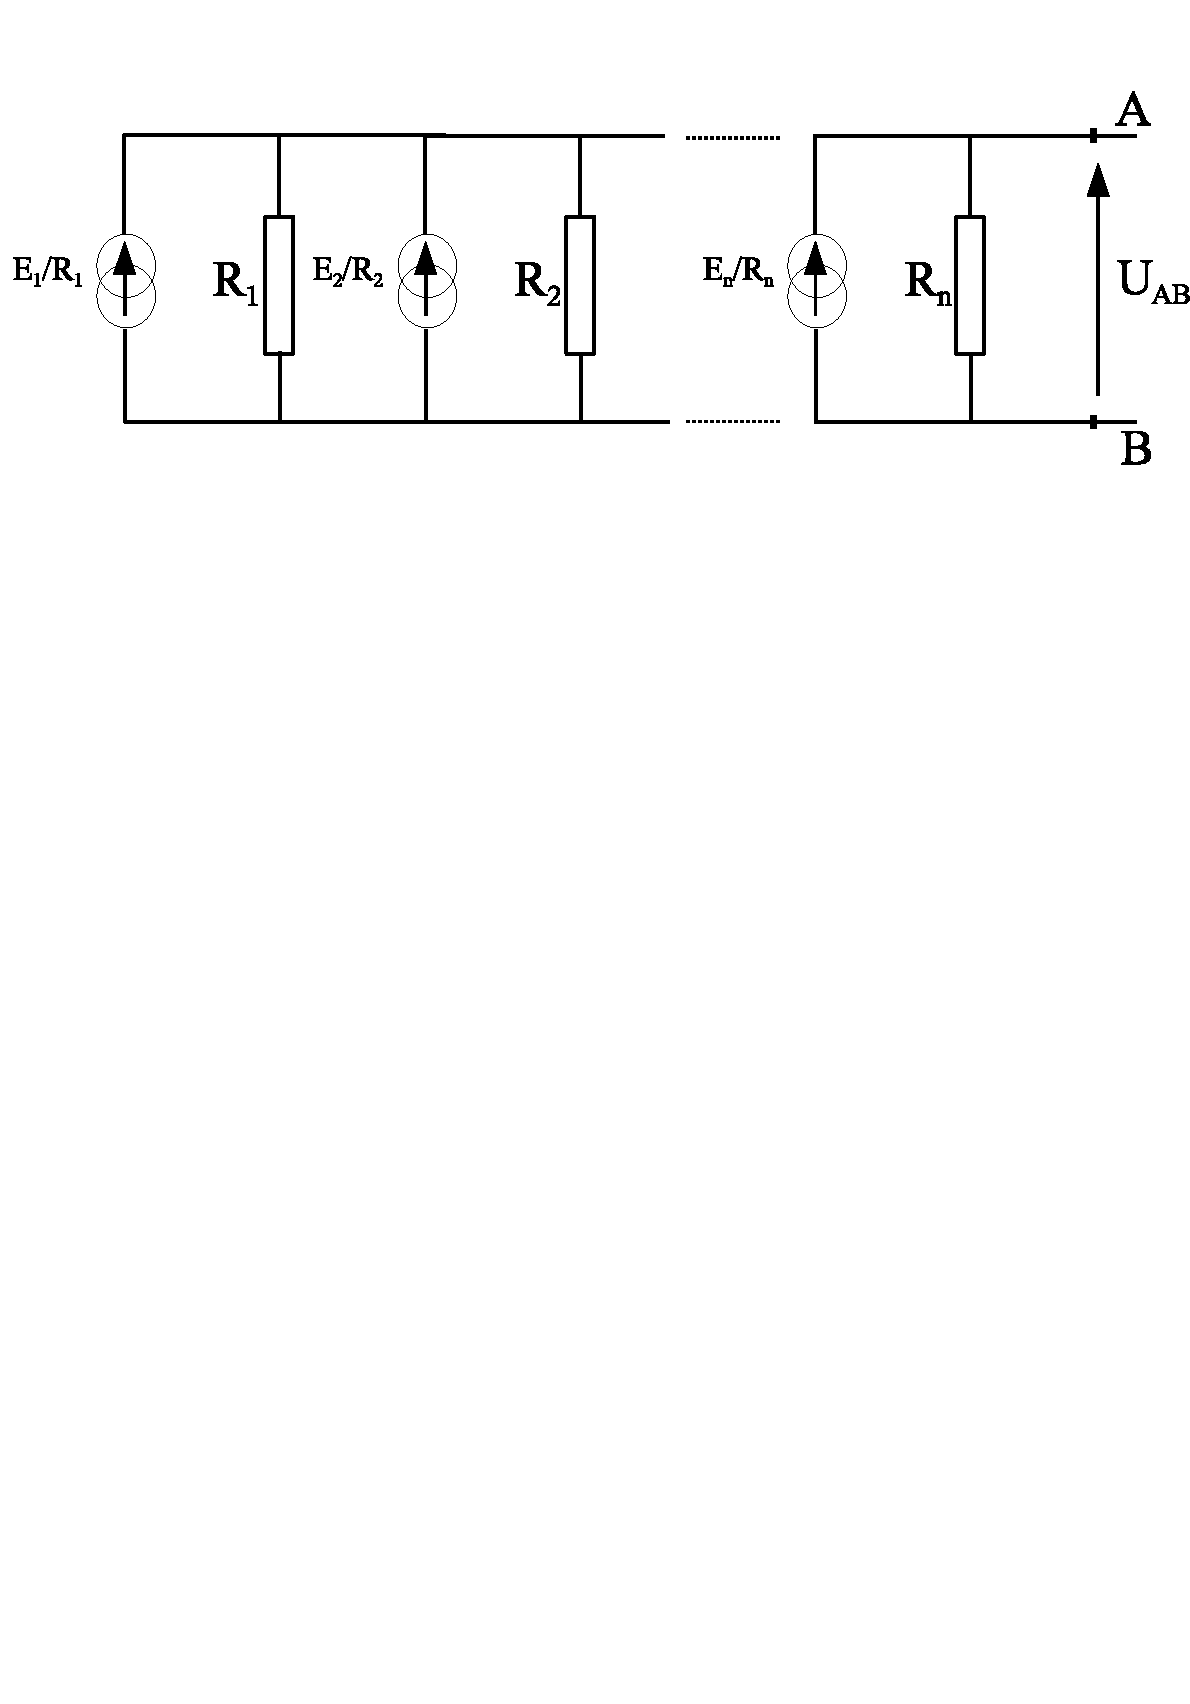
\includegraphics[clip=true,viewport=0cm 21cm 21cm 27.5cm,scale=0.7]{./figures/methode_millmann_dual.pdf}
\caption{Circuit dual �quivalent.}
\end{center}
\end{figure}

$$\frac{1}{R}=\sum_{i} \frac{1}{r_{i}}$$
$$I=\sum_{i}I_{i}=\sum_{i}\frac{e_{i}}{r_{i}}$$
$$U_{AB}=RI$$

\subsection{Th�or�me de Th�venin}

\begin{enon}
Tout r�seau lin�aire compris entre deux bornes $A$ et $B$, aussi compliqu� soit-il, est �quivalent � un g�n�rateur unique de f�m $e$ et de r�sistance interne $r$ telles que :
\begin{enumerate}
\item $e = E$ est la tension mesur�e entre $A$ et $B$ � l'aide d'un voltm�tre ;
\item $r = R_{eq}$, o� $R_{eq}$ est la r�sistance �quivalente du r�seau, obtenue en posant que toutes les forces �lectromotrices (f.�.m.) et les forces contre-�lectromotrices (f.c.�.m.) sont nulles.
\end{enumerate}
\end{enon}

On ne s'int�resse qu'au fonctionnement d'un dip�le �quivalent $(AB)$ d'un r�seau. Si ce dip�le �quivalent est une source de tension, on l'appelle g�n�rateur de Th�venin. Cette m�thode est donc tr�s utile pour d�terminer des g�n�rateurs �quivalents de circuits complexes pour lesquels les lois de Kirchhoff deviennent inadapt�es, \cad lorsque le nombre d'inconnues dans le syst�me d'�quations devient trop grand.


 \begin{figure}[h]
\centering
\subfigure[Sch�ma initial]{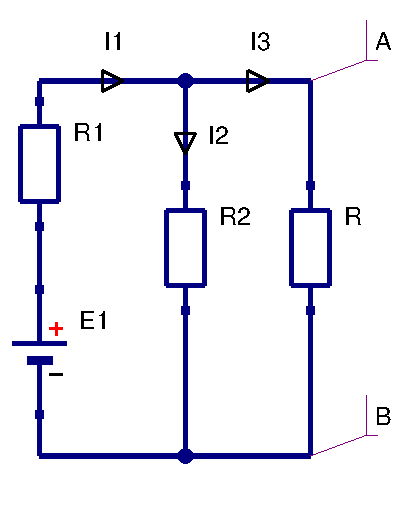
\includegraphics[width=5cm]{./figures/sch_thev_1-crop.pdf}}
\subfigure[]{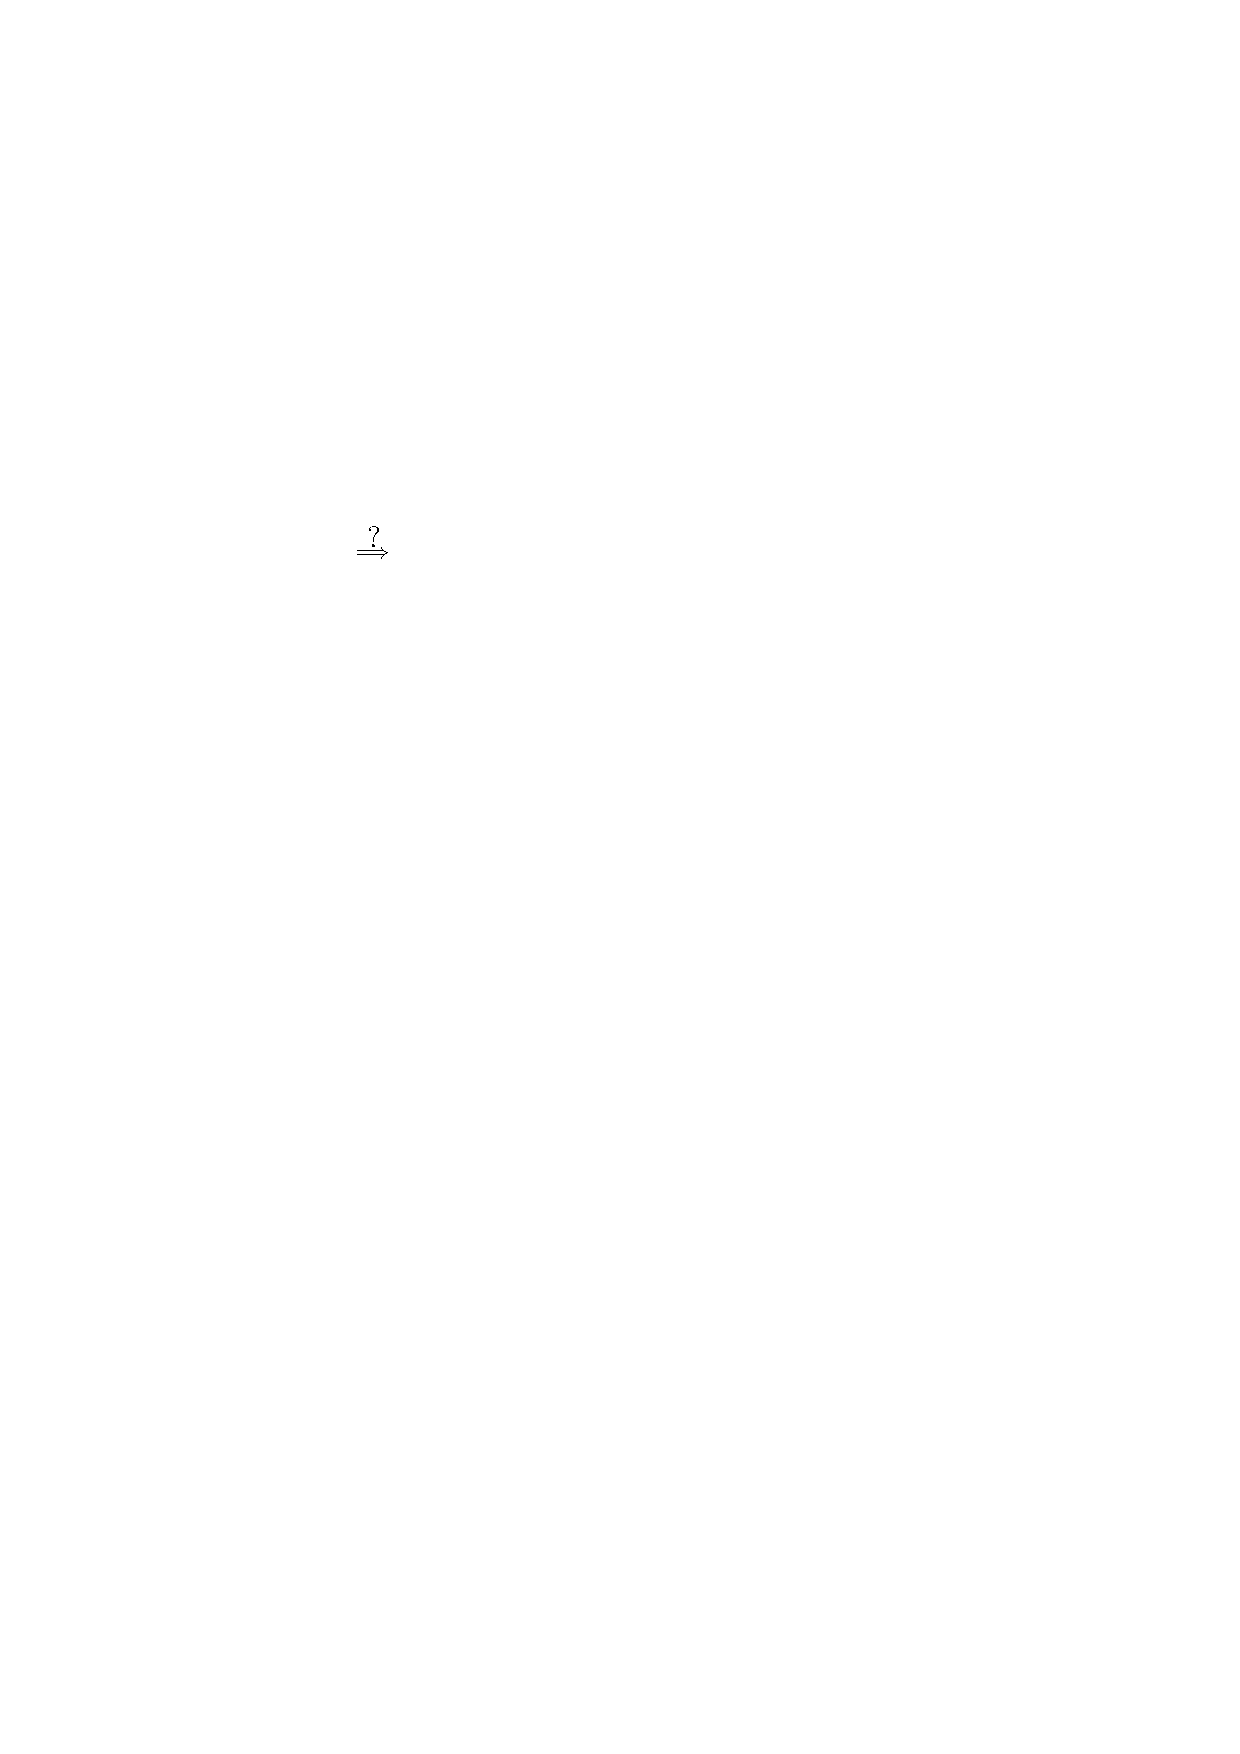
\includegraphics[width=2cm]{./figures/implique.pdf}}
\subfigure[G�n�rateur de Th�venin �quivalent]{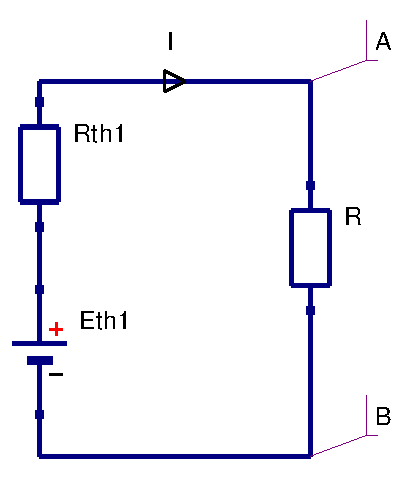
\includegraphics[width=5cm]{./figures/sch_thev_5-crop.pdf}}
\caption{Exemple d'un sch�ma pour l'application du th�or�me de Th�venin.}
\label{sch_thev_1}
\end{figure}

\begin{bex}[Cicuit �quivalent]

La figure \ref{sch_thev_1} pr�sente une r�sistance $R$ aliment�e par un circuit comprenant un g�n�rateur $E$ muni de sa r�sistance propre $R1$ et d'une r�sistance suppl�mentaire $R2$ en parall�le. On cherche � conna�tre le g�n�rateur �quivalent aux bornes de $R$ entre $A$ et $B$.

% \begin{figure}[h]
% \begin{center}
% 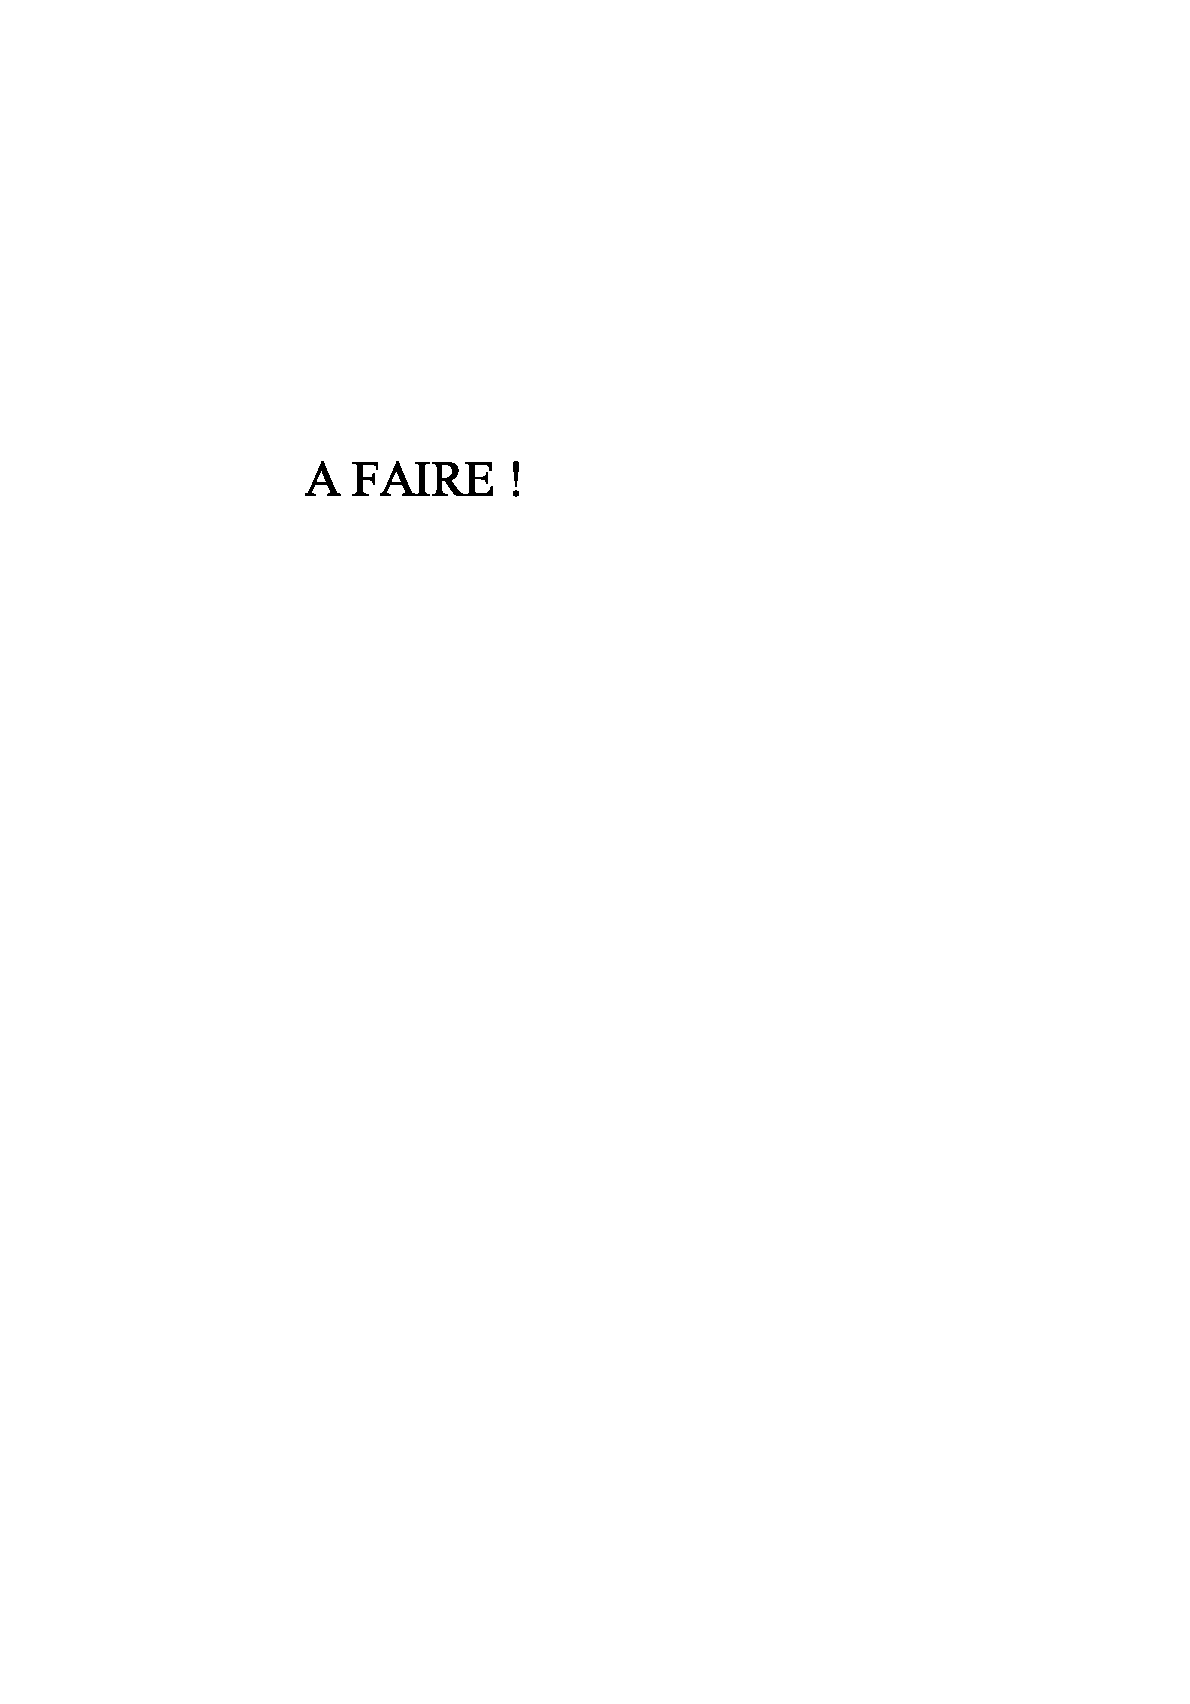
\includegraphics[clip=true,viewport=0cm 18cm 20cm 27cm,scale=0.38]{./figures/a_faire.pdf}
% \caption{Exemple de circuit charg�.}
% \end{center}
% \end{figure}

L'application du th�or�me de Th�venin comporte 4 �tapes.

\begin{enumerate}

\item On d�connecte le dip�le de charge (cf. \ref{sch_thev}(a)):

\begin{figure}[h]
\centering
\subfigure[$1^{\'ere}$ �tape - enl�vement de la charge]{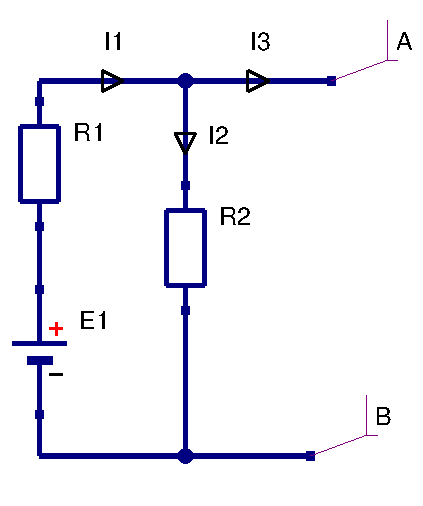
\includegraphics[width=5cm]{./figures/sch_thev_2-crop.pdf}}
\hspace{2cm}
\subfigure[$2^e$ �tape - calcul de la r�sistance �quivalente]{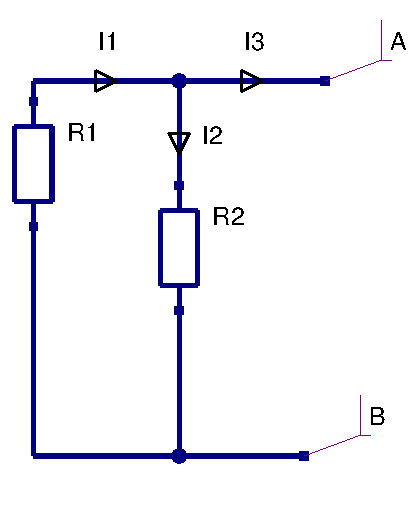
\includegraphics[width=5cm]{./figures/sch_thev_3-crop.pdf}}\\
\subfigure[$3^e$ �tape - calcul de la tension � vide]{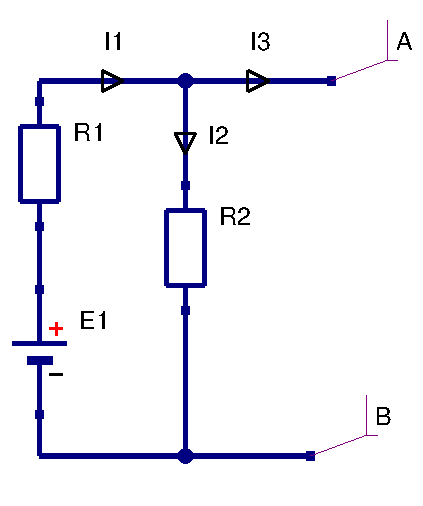
\includegraphics[width=5cm]{./figures/sch_thev_2-crop.pdf}}
\hspace{2cm}
\subfigure[$4^e$ �tape - remplacement du dip�le par le g�n�rateur de Th�venin �quivalent]{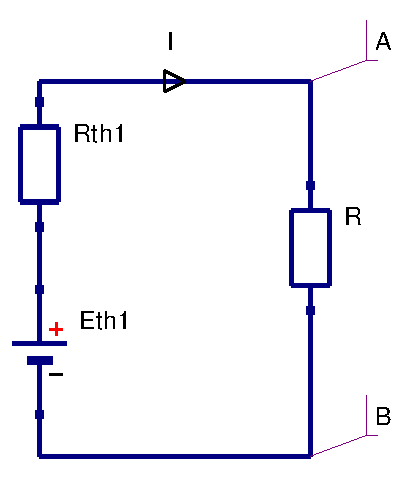
\includegraphics[width=5cm]{./figures/sch_thev_5-crop.pdf}}
\caption{Etape du calcul d'un g�n�rateur de Th�venin �quivalent.}
\label{sch_thev}
\end{figure}


\item On supprime toutes les sources et on calcule la r�sistance �quivalente $R_{th}$ (cf. \ref{sch_thev}(b)):

\begin{equation}\label{r_th}
R_{th} = \frac{R_{1}R_{2}}{R_{1}+R_{2}}
\end{equation}

\item On r�tablit les sources et on calcule la tension � vide $E{th}=V_A-V_B$ qui donnera la tension du g�n�rateur �quivalent (cf. \ref{sch_thev}(c)):

D'apr�s la loi d'Ohm $I1=I2$ et $I3=0\ A$, d'o�:

\begin{equation}
I1=\frac{E1}{R1+R2}\end{equation}

On en d�duit d'apr�s la loi des mailles :

\begin{equation}\label{e_th}
 E_{th} = V_A - V_B = R2.I2 =  \frac{R2.E1}{R1+R2}
\end{equation}

\item On remplace le dip�le de commande par le g�n�rateur de Th�venin �quivalent (cf. \ref{sch_thev}(d)) o� on utilise les quantit�s donn�es aux �quations \ref{r_th} et \ref{e_th}.

\end{enumerate}

\textbf{Remarque :} ATTENTION ! Ceci est un example et non un cas g�n�ral. Seule la m�thode en 4 �tapes s'applique mais les �quations diff�rent selon les cas. On doit syst�matiquement utiliser les lois de Kirchhoff pour d�terminer les lois de tension et de courant.
\end{bex}


\subsection{Th�or�me de Norton}

C'est la forme duale du th�or�me de Th�venin. Le g�n�rateur de tension est remplac� par un g�n�rateur de courant.

\begin{figure}[h]
\begin{center}
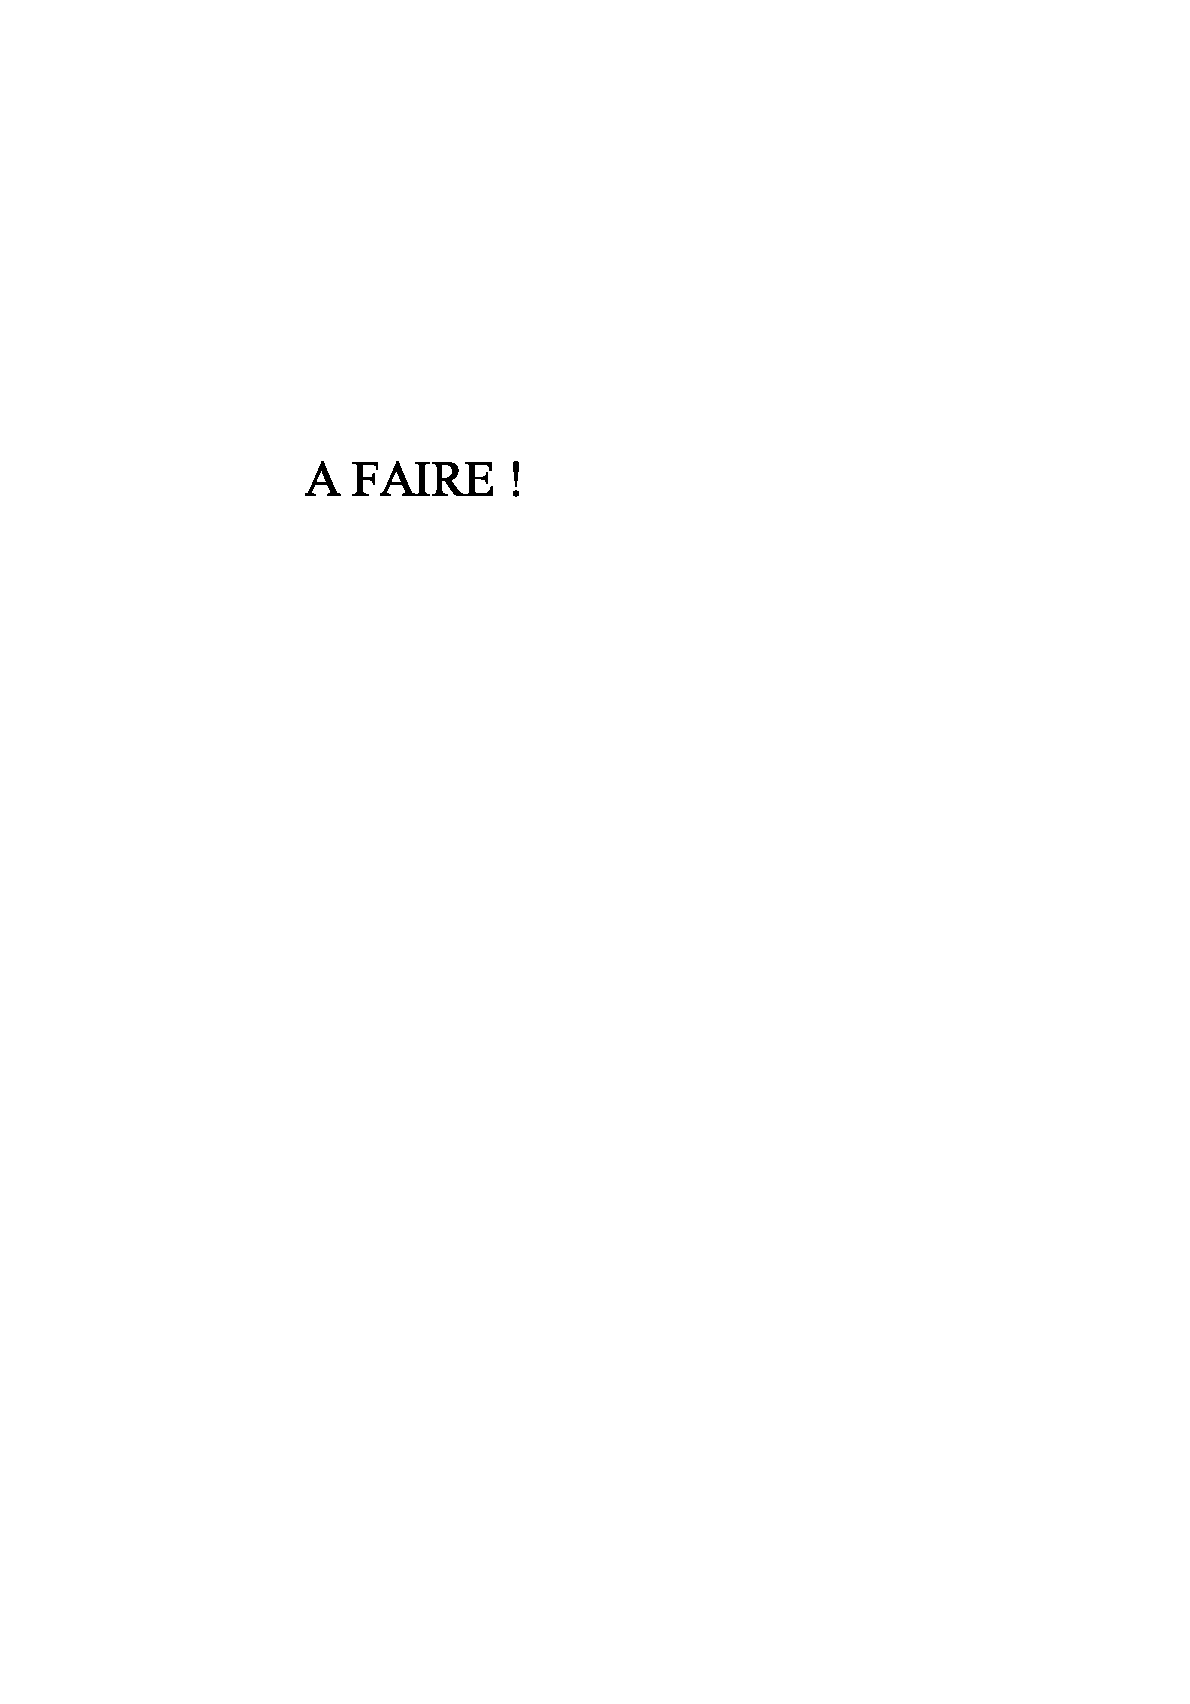
\includegraphics[clip=true,viewport=0cm 18cm 20cm 27cm,scale=0.38]{./figures/a_faire.pdf}
\caption{G�n�rateur de Norton.}
\end{center}
\end{figure}

La r�sistance est d�termin�e de la m�me fa�on. Le courant est le courant de court-circuit pratiqu� aux bornes du dip�le de commande.

\textit{Suite � venir...}

\cleardoublepage

\chapter{Electromagn�tisme}\label{chap_elecmagn}

\section{Introduction}
L'�lectrostatique nous a permis d'introduire les notions d'action � distance entre particules charg�es au repos. Cette description cesse d'�tre compl�te lorsque les charges sont en mouvement. Il y a alors apparition de nouveaux types d'interactions qui constituent une partie de la th�orie de l'�lectromagn�tisme : la \textbf{magn�tostatique}.

\section{Le champ magn�tique}

\subsection{Pr�ambule}

Les effets magn�tiques proc�dent d'une \textbf{interaction � distance}. Comme en �lectrostatique, on doit donc pouvoir en d�duire ses effets � l'aide d'un champ qui sera un outil math�matique. La connaissance de ce champ suffira � conna�tre tous les effets magn�tiques ind�pendamment des sources qui l'ont cr��.

\subsection{Topographie du champ magn�tique}

Le champ magn�tique est une grandeur vectorielle, on la note $\vec{B}$. Voici quelques exemples de situations mettant en jeu un champ magn�tique dont on trace les lignes de flux.

\begin{itemize}
 \item Champ terrestre
 \item Aimant droit
 \item Aimant en U
 \item Fil infini
 \item Spire
\end{itemize}

\subsection{D�finition du champ magn�tique}

Le champ magn�tique $\vec{B}$ est d�fini par son action sur les particules charg�es en mouvement.

\subsubsection{Quelques exp�riences}

\paragraph{Canon � �lectrons :}ampoule sous vide ($H_2,\ 10{-5}\ \mathrm{Bar}$). Les �lectrons projet�s depuis l'�lectrodes sont d�vi�s par le champ magn�tique impos� (variable dans le cas du tube cathodique de la t�l�vision).
\paragraph{Bobine de Helmholtz :}champ uniforme. $\vec{v_0}$ est orientable.

\subsubsection{Observations}

\begin{figure*}[ht]
\begin{center}
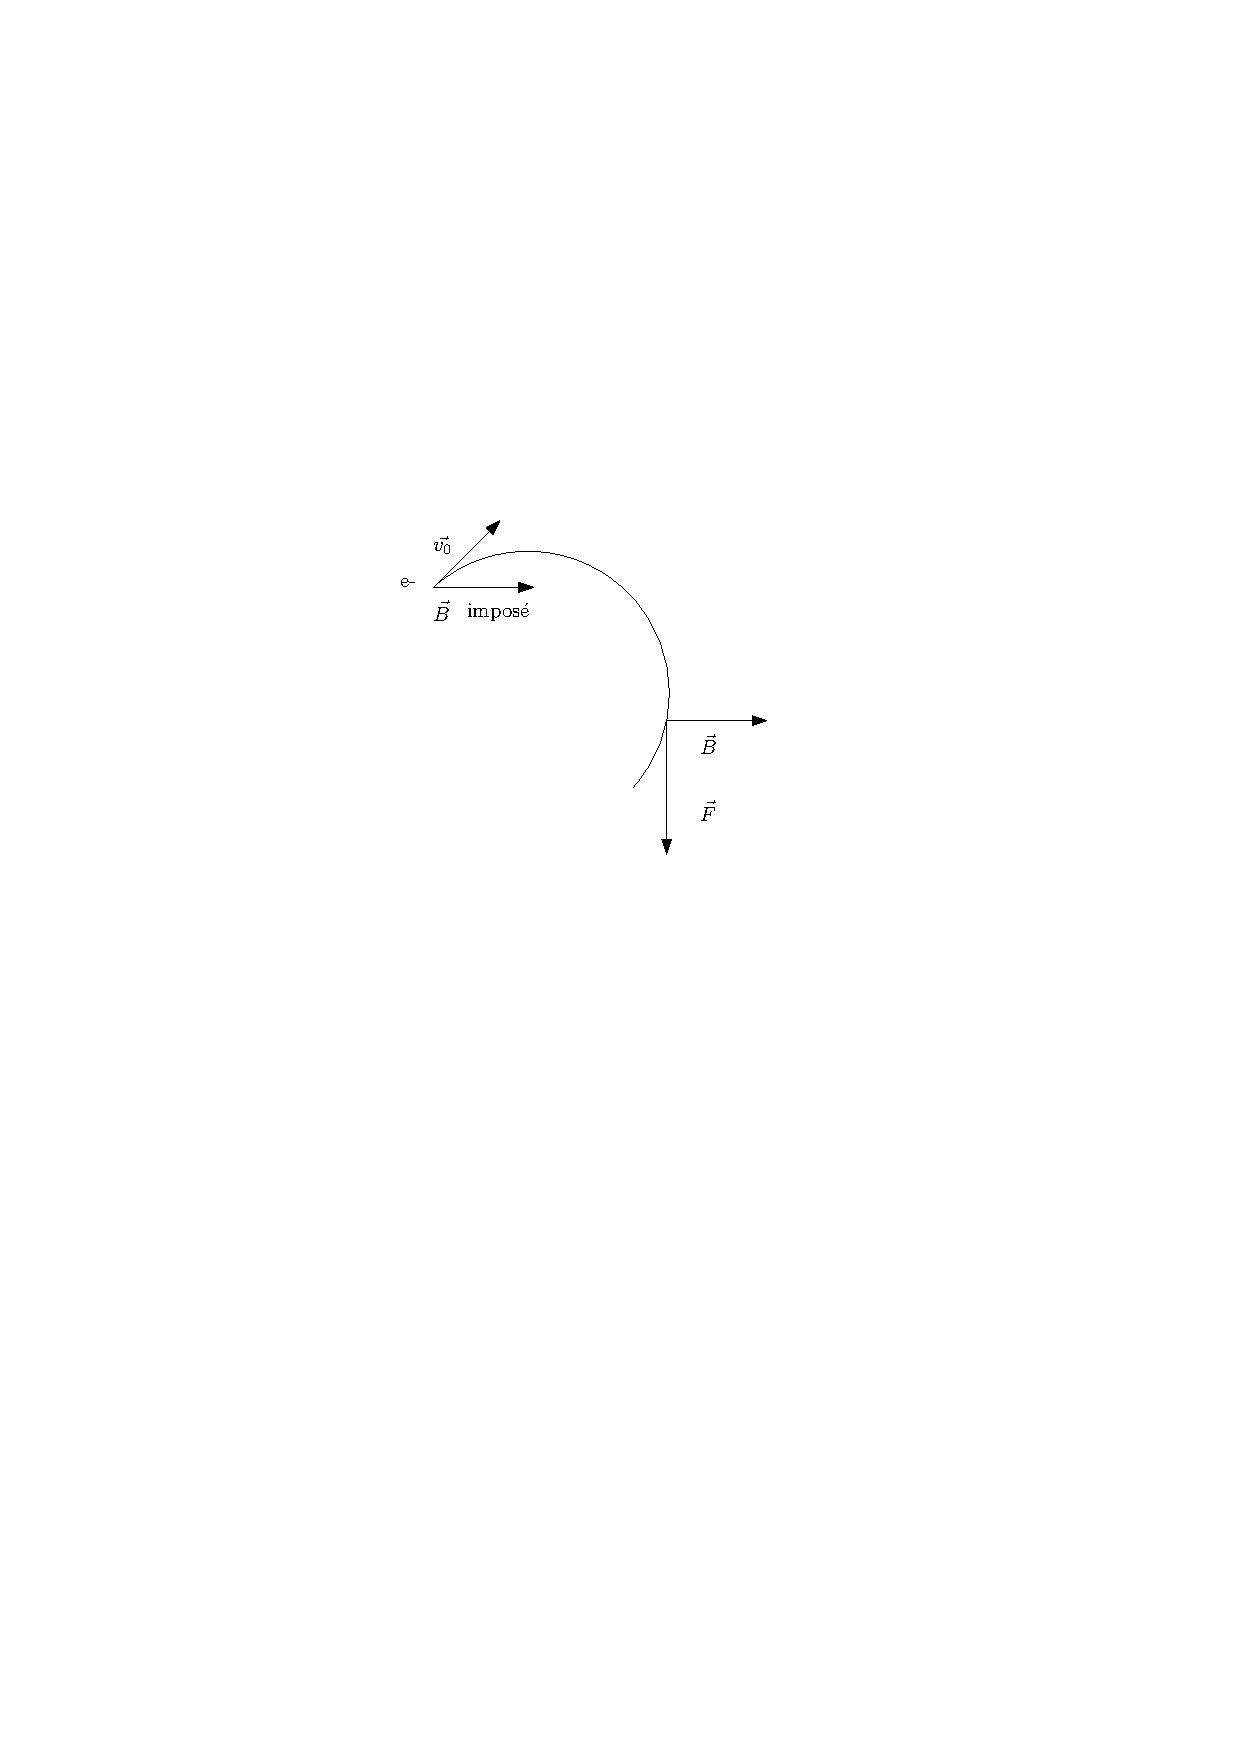
\includegraphics[width=6cm]{./figures/champ_magn1.pdf}
\label{biot_savart}
\end{center}
\end{figure*}

Soit un �lectron �voluant dans l'espace � une vitesse $\vec{v_0}$ dans un champ magn�tique $\vec{B}$ (voir la figure \ref{biot_savart}). Une force magn�tique $\vec{F}$ appara�t et nous pouvons faire les observations suivantes:


\begin{itemize}
 \item $\vec{F}\bot\vec{B}$.
 \item $\vec{F}\bot\vec{v_0}$.
 \item $\vec{F}=\vec{0}$ si $\vec{v}//\vec{B}$.
 \item Si on inverse $\vec{B}$, $\vec{F}$ s'inverse.
 \item Si $q\times 2$, $F\times 2$
\end{itemize}

On d�duit de ces observations une loi de force magn�tique $\vec{F}_{magn}$ dite \textbf{Force de Lorentz} telle que :

\begin{equation}
 \vec{F}_{magn}=q \vec{v}\wedge\vec{B_{ext}}
\end{equation} 


Force de Lorentz g�n�ralis�e :

\begin{equation}
 \vec{F}_{magn}=q (\vec{E} + \vec{v}\wedge\vec{B})
\end{equation} 

\subsection{Loi de Biot et Savart}

\begin{equation}
 d\vec{B}=\frac{\mu_0 I \vec{dl}\wedge \vec{AM}}{4\pi AM^3}
\end{equation}

O� $\mu_0$ est une constante fondamentale, appel�e perm�abilit� magn�tique du vide.

En vertu du principe de superposition des champs magn�tiques, le champ total cr�� par l'ensemble des circuits contenus dans l'espace s'�crit :

\begin{equation}
 \vec{B}=\int_{circuits} \frac{\mu_0 I \vec{dl}\wedge \vec{AM}}{4\pi AM^3}
\end{equation}

\subsection{Champ magn�tique cr�� par un fil rectiligne}

...

\begin{equation}\label{Br_fil}
 B(r)=\frac{\mu_0 I}{2\pi r}
\end{equation}

A l'avenir, on utilisera le th�or�me d'Amp�re.

\subsection{Action d'un champ $\vec{B}$ sur un conducteur parcouru par un courant - Force de Laplace}

Le champ $\vec{B}$ exerce une force $\vec{dF}$ sur l'�l�ment $d\tau$ telle que :

\begin{equation}
 \vec{dF} = \vec{J}\wedge\vec{B}. d\tau
\end{equation}

$\frac{\vec{dF}}{d\tau}$ est la densit� volumique de force.





\subsection{Le th�or�me d'Amp�re}

Nous avons vu en �lectrostatique que l'�l�ment de circulation du champ �lectrique $\vec{E}$ sur un �l�ment de de chemin $\vec{dl}$ se d�finissait par:

\begin{equation*}
 dC = \vec{E}.\vec{dl}
\end{equation*}

De la m�me fa�on, nous d�finissons un �l�ment de circulation du champ magn�tique par :
\begin{equation*}
 dC = \vec{B}.\vec{dl}
\end{equation*}

La circulation totale en suivant une ligne $\Gamma$ s'�crit :

\begin{equation*}
 C=\oint_\Gamma \vec{B}.\vec{dl}
\end{equation*}

Consid�rons le chemin $\Gamma$ ferm�, constitu� du cercle de centre $O$ et de rayon $r$ orient� comm indiqu� sur la figure \ref{sch_amp1}. En chaque point du cercle, $\vec{B}$ et $\vec{dl}$ sont colin�aires et de m�me sens. L'�l�ment de circulation est donc simplement $dC=\Vert\vec{B}\Vert \times \Vert\vec{dl}\Vert$.

Puisque B est constant sur tout le cercle et ne d�pend que du rayon $r$, la circulation totale du champ magn�tique sur le cercle est $2\pi r B(r)$. D'apr�s l'expression \ref{Br_fil} de $B(r)$, on en d�duit :

\begin{equation}\label{th_ampere}
 C = \oint_\Gamma \vec{B}.\vec{dl} = \mu_0 I
\end{equation}


\subsection{Travail des forces de Laplace}

Un circuit parcouru par un courant $I$ fix� dans un champ magn�tique $\vec{B}$ sera soumis � une force de Laplace telle que :

\begin{equation}\label{laplace}
 \vec{F} = I \int \vec{dl}\wedge\vec{B}
\end{equation} 


\section{L'induction}

\subsection{Introduction}

2 exp�riences

G�n�ralisation :

\begin{equation}
 \vec{E_m}=-\frac{\partial \vec{A}}{\partial t} + \vec{v}\wedge\vec{B}
\end{equation}

et

\begin{equation}
 \vec{E_{tot}}=\vec{E_0}+\vec{E_m}
\end{equation} 


\subsection{Tension aux bornes d'un conducteur}

\begin{equation}
 V_C - V_D = R_{CD}I_{CD}-e_{CD}
\end{equation}


\subsection{Calcul de la force �lectromotrice}

Cas du circuit ferm� :

\begin{equation}
 e = -\frac{d\Phi}{dt}
\end{equation} 

\subsection{Auto-induction}

On suppose $\vec{B_0}=\vec{0}$, mais $i(t)$ est non nul dans le circuit. Alors $i(t)$ cr�e un champ propre $B(t)$ impliquent un flux $\Phi_{propre}$ tel que:

\begin{equation}
 \Phi_{propre}=L i(t)
\end{equation} 
 o� $L$ est l'inductance de la spirale en Henry.

 Il est alors cr��e une f.e.m. induite $e_{induite}$ telle que:

 \begin{equation}
  e_{induite}=-\frac{d \Phi_{propre}}{dt}=-L\frac{di(t)}{dt}
 \end{equation}

\section{Le sol�no�de}

Le sol�no�de est mod�lis� par une s�rie de $N$ spires de rayons $R$, de m�me axe, parcourues par un m�me courant $I$ et dispos�es r�guli�rement sur une longueur $2a$. On note $O$ le centre du sol�no�de, et $A$ et $B$ ses extr�mit�s.

On conna�t le champ magn�tique cr�� par une spire de courant sur son axe. On peut alors en d�duire le champ cr�� par le sol�no�de sur son axe :

\begin{equation}
 B(z)=\mu_0 N I \frac{\Omega_A - \Omega_B}{4 \pi}
\end{equation}

o� $\Omega_A$ et $\Omega_B$ sont les angles solides sous lequel on voit respectivement la face $A$ et la face $B$ depuis la distance $z$ par rapport � $O$, et $\mu_0$ est la perm�abilit� magn�tique du vide.

Au centre du sol�no�de, c'est-�-dire en $z=0$, cette formule devient :

\begin{equation}
 B(0)=\mu_0 N I \frac{a}{\sqrt{a^2 + R^2}}
\end{equation}

On peut montrer qu'il est possible de d�terminer le champ magn�tique dans tout l'espace ($\vec{B}(r,z)=B_z(r,z)\vec{u_z}+B_r(r,z)\vec{u_r}$) � partir du champ magn�tique sur l'axe ($B(0,z)$ not� $F(z)$) gr�ce aux relations suivantes :

\begin{eqnarray}
    B_z(r,z) & = & F(z) - \frac{1}{4} r^2 F''(z)\\
    B_r(r,z) & = & -\frac{1}{2}r F '(z) + \frac{1}{16} r^3 F'''(z).
\end{eqnarray} 

On s'aper�oit alors que ce champ est quasi-homog�ne dans tout le volume d�limit� par le sol�no�de. Cela correspond � des lignes de champ quasi-parall�les entre elles. A l'ext�rieur du sol�no�de, le champ est analogue � celui d'un aimant: il pr�sente un p�le nord et un p�le sud. Il est cependant tr�s faible.

\subsection{Etablissment et suppression du courant dans un sol�no�de}

\subsection{Analyse d'un circuit RL}

\subsubsection{Etablissment du courant}

\subsubsection{Suppression du courant}






\chapter{Courants Variables}\label{chap_cour_var}

\section{Repr�sentation complexe des grandeurs sinuso�dales}

\section{Imp�dances complexes}

L'imp�dance est d�finie comme le rapport de la tension $u(t)$ (en V) et du courant $i(t)$ o� $u(t)=U_0 e^{j\omega t+\phi_i}$ avec $U_0$ la tension max et $\omega$ la pulsation du signal, et o� $u(t)=I_0 e^{j\omega t+\phi_u}$ avec $I_0$ est l'intensit� max. On �crit :

\begin{equation}\label{imp_comp}
 Z=\frac{u}{i}
\end{equation}

\subsection{R�sistance}

Soit $Z_R$ l'imp�dance complexe d'une r�sistance. D'apr�s l'�quation \ref{imp_comp}, $Z_R$ est la r�sistance r�elle du dip�le telle que:

\begin{equation}
 Z_R=\frac{U_0}{I_0}=R
\end{equation}

\subsection{Capacitance}

Soit $Z_C$ l'imp�dance complexe d'une capacitance (condensateur). On sait que $i(t)=C \frac{\partial u(t)}{\partial t}$. Or $\frac{\partial u(t)}{\partial t} = j\omega U_0 e^{j\omega t}$. On en d�duit d'apr�s l'�quation \ref{imp_comp}:

 \begin{equation}
  Z_C=\frac{1}{j C\omega}
 \end{equation}

\subsection{Inductance}

Soit $Z_L$ l'imp�dance complexe d'une inductance (sol�no�de). On sait que $u(t)=L \frac{\partial i(t)}{\partial t}$. Or $\frac{\partial i(t)}{\partial t} = j\omega I_0 e^{j\omega t}$. On en d�duit d'apr�s l'�quation \ref{imp_comp}:

 \begin{equation}
  Z_L=j L\omega
 \end{equation}

\subsection{Puissances}

\subsubsection{Puissance instantan�e}

\begin{equation}
 p=ui\ \ \ (\mathrm{W = J.s^{-1}})
\end{equation}

\subsubsection{Puissance active (absorb�e)}

La puissance active correspond � l'�nergie moyenne consomm�e par unit� de temps \cad � la \textbf{puissance moyenne consomm�e} :

\begin{equation}
 P=<p>=\frac{1}{T}\int_0^T p\ dt
\end{equation}

d'o�, en r�gime sinuso�dal:

\begin{equation}
 P=\frac{U_0 I_0}{2} \cos \phi
\end{equation}

soit,

\begin{equation}
 P=U I \cos \phi
\end{equation}

o� $I=\frac{I_0}{\sqrt{2}}$ et $U=\frac{U_0}{\sqrt{2}}$ sont respectivement la valeur efficace du courant et la valeur efficace de la tension dans le circuit.

\subsubsection{Puissance r�active}

\begin{equation}
 Q=\frac{U_0 I_0}{2} \sin \phi = U I \sin \phi
\end{equation}

\subsubsection{Puissance apparente}

\begin{eqnarray}
 S & = & U I\\
 S & = & \sqrt{P^2 + Q^2}
\end{eqnarray}


\section{Etude de cas}

\subsection{Circuit RLC}

\subsection{Th�or�me de Th�venin en notation complexe}

\subsection{Th�or�me de Norton en notation complexe}



%%%%%%%%%%%%%%%%%%%%%%%

\newpage
\begin{center}
\bold{\emph{\underline{RESUME DU PROGRAMME D'ELECTRICITE (20 heures)}}}
\end{center}

\bigskip

\bold{\emph{ELECTROSTATIQUE}}

\begin{small}
\begin{enumerate}
\item{Rappels}
	G�n�ralit�s~: charge �lectrique �l�mentaire ; corps charg�s. Loi de Coulomb. Principe de superposition. Champ �lectrique ; exemples.
\item{Etude du champ �lectrique}
	D�finition du flux. Th�or�me de Gauss. Application~: calcul du champ cr�� par une distribution uniforme (rectiligne, plane, sph�rique).
\item{Potentiel}
	Travail des forces �lectriques ; d�finition du potentiel. Relation entre potentiel et champ. Calculs de potentiels simples.
\item{Condensateurs}
	\begin{itemize}
	\item Charge des condensateurs en �quilibre. D�finition et capacit� du condensateur.
	\item Condensateur en pr�sence d'un di�lectrique.
	\item Energie emmagasin�e par un condensateur,
	\item Association de condensateurs
	\end{itemize}
\item Notions sur les �lectrets
\end{enumerate}
\end{small}

\bold{\emph{COURANTS CONTINUS}}

\begin{small}
\begin{enumerate}
\item{Rappels}
	G�n�ralit�s~: densit� de courant, courant, intensit�, diff�rence de potentiel. Loi d'Ohm, r�sistivit� et r�sistance des conducteurs. Association de r�sistances. Loi de Joule.
\item{G�n�rateurs - R�cepteurs}
	\begin{itemize}
	\item G�n�rateur. 	D�finition ; f.e.m., r�sistance interne. G�n�rateur de tension, g�n�rateur de courant. Charge adapt�e. Association. G�n�rateur chimique~: Description et fonctionnement d'une pile. Exemples. Potentiel d'�lectrode.
	\item R�cpeteur. D�finition ; f.e.m., r�sistance interne. Association.
	\end{itemize}
\item{R�seaux}
	D�finitions et conventions de signe internationale. Lois de Kirchoff ; loi des noeuds, loi des mailles. Mise en �quation et r�solution de r�seaux simples. Th�or�me de superposition. Th�or�me de Th�venin et th�or�me de Norton, applications.\\
\end{enumerate}
\end{small}

\bold{\emph{ELECTROMAGNETISME}}

\begin{small}
\begin{enumerate}
\item{Rappels}
	\begin{itemize}
	\item Magn�tostatique
		Origine du champ magn�tique, force de Lorentz.
		Action d'un champ sur un circuit~: loi de Laplace ; exemples.
		Champs cr��s par des courants ; exemples.
		Int�raction entre circuits~: relation entre flux magn�tiques et courants ; coefficients d'inductance. Propri�t�s des aimants permanents.
	\item Induction
		Description du ph�nom�ne. F.e.m. d'induction ; loi de Faraday. Auto-induction ; tension aux bornes d'une bobine. Induction mutuelle ; tension aux bornes de bobines coupl�es.
	\end{itemize}
\item{Etude du champ magn�tique}
Loi de Biot et Savart~: calcul d'un champ cr�� par un fil rectiligne. Th�or�me d'Amp�re. Application au sol�no�de. Notion de conservation du flux magn�tique.\\
\end{enumerate}
\end{small}

\bold{\emph{COURANTS VARIABLES (Quasi-stationnaires)}}

\begin{small}
\begin{enumerate}
\item{Circuits en r�gime transitoire}
	Charge et d�charge d'un condensateur. Etablissement et ruptur du courant dans une bobine.
\item{Circuits en r�gime sinuso�dale forc�}
	G�n�ralit�s. Repr�sentation complexe des grandeurs sinuso�dales. Imp�dance complexe d'�l�ments passifs simples. Association d'imp�dances. Etude du circuit r�sonnant RLC ; r�sonance, surtension, facteur de qualit�. G�n�rateur de tension sinuso�dale~: f.e.m. et imp�dance interne complexes. Puissance et adaptation d'imp�dance.
	R�seaux~: lois de Kirchoff, th�or�mes de Th�venin et Norton en notation complexe, exemples.
\end{enumerate}
\end{small}



\end{document}